\setcounter{chapter}{2}


\chapter{Second and Higher Order Linear Differential Equations}\label{chap:higher-order}
\mtcsetoffset{minitoc}{-1em}
% \mtcsetpagenumbers{minitoc}{off}

\minitoc
\section{Introduction}
The $n^\text{th}$ order linear differential equations are of the form
\begin{equation}\label{eq:nonhomogeneous-0}
	a_n(x)y^{(n)} + a_{n-1}(x)y^{(n-1)} + \cdots + a_1(x)y' + a_0(x)y = f(x)
\end{equation}
where   the  functions \( a_0(x), \dots, a_{n-1}(x), a_n(x) \) and   \( f(x) \) are continuous on some interval \( I .\)
We say that \eqref{eq:nonhomogeneous-0} is \textbf{\textit{homogeneous}}\index{homogeneous} on $I$ if $f(x) = 0$ for all $x$ in $I$ and \textbf{\textit{nonhomogeneous}}\index{nonhomogeneous} on $I$ if $f(x)\ne 0$ for some $x$ in $I.$  We will usually have $a_n(x) \ne 0$ on $I.$ If $a_n(x=0$ for some point $x$ of $I,$ we will simply restrict our attention to a smaller interval, denoted again by \(I\), on which $a_n(x) \ne 0.$  With these consideration, \eqref{eq:nonhomogeneous-0} can be   rewritten in the form
\begin{equation}\label{eq:nonhomogeneous0}
	y^{(n)} + a_{n-1}(x)y^{(n-1)} + \cdots + a_1(x)y' + a_0(x)y = f(x),
\end{equation}
 \( a_0(x), \dots, a_{n-1}(x) \) and   \( f(x) \) are continuous on some interval \( I .\) This is achieved by dividing both sides of \eqref{eq:nonhomogeneous-0} by $a_n(x)$ to obtain
 \[y^{(n)}+\frac{a_{n-1}(x)}{a_n(x)}y^{(n-1)}+ \cdot+\frac{a_1(x)}{a_n(x)}y'+\frac{a_0(x)}{a_n(x)}y= \frac{f(x)}{a_n(x)} \]
  and redefining the   functions \[ \frac{a_{n-1}(x)}{a_n(x)}, \dots,\frac{a_1(x)}{a_n(x)}, \frac{a_0(x)}{a_n(x)}, \frac{f(x)}{a_n(x)} \] as \[ a_{n-1}(x), \dots,a_1(x), a_0(x), f(x), \] respectively.
 
\begin{definition}[Solution]\label{def:solutions}
	A function $y = \phi(x)$ defined on $I$ is said to be a \textbf{\textit{solution}} of \eqref{eq:nonhomogeneous0} if 
	\[\phi^{(n)}(x) + a_{n-1}(x)\phi^{(n-1)}(x) + \cdots + a_1(x)\phi'(x) + a_0(x)\phi(x) = f(x)\] for all $x$ in $I,$ that is, if
	\eqref{eq:nonhomogeneous0} is satisfied for all $x$ in $I$ when we substitute $\phi(x)$  for $y.$
\end{definition}

%In Definition~\ref{def:solutions},  the derivatives of $\phi(x)$ at the endpoints (if any) of \(I\) are interpreted as one-sided derivatives.

\begin{remark}
	In Definition~\ref{def:solutions}, we note the following.
	\begin{enumerate}[label=(\roman*), noitemsep]
		\item Derivatives of $\phi(x)$ at the endpoints (if any) of \(I\)  are understood as one-sided.
		\item Solutions $y = \phi(x)$ may be complex-valued, though real solutions are preferred in  applications. For $\phi(x) = \phi_1(x) + i \phi_2(x)$ with real $\phi_1$ and $\phi_2$, 
		\[
		\phi'(x) = \phi_1'(x) + i \phi_2'(x),
		\]
		where $i = \sqrt{-1}$, and higher derivatives are computed similarly.
	\end{enumerate}
\end{remark}


%\begin{remark}
%	In Definition~\ref{def:solutions}, we note the following:
%	\begin{enumerate}[label=(\roman*), noitemsep]
%		\item Derivatives of $\phi(x)$ at the endpoints (if any) of \(I\) are interpreted as one-sided derivatives.
%		\item The solution $y = \phi(x)$ are allowed to be complex-valued although real-valued functions are desirable for solutions. If $\phi(x) = \phi_1(x) + i \phi_2(x)$, with real-valued $\phi_1$ and $\phi_2$, then 
%		\[
%		\phi'(x) = \phi_1'(x) + i \phi_2'(x),
%		\]
%		 and higher order derivatives are computed similarly.
%		Here $i = \sqrt{-1}$ is the imaginary unit.
%	\end{enumerate}
%\end{remark}

\begin{definition}[Initial Value Problem]
	Let   \( a_0(x), \dots, a_{n-1}(x), f(x) \)  be continuous functions on some interval \( I \), $x_0$ be a point in $I$, and $y_1,\dots, y_{n-1}$ be fixed numbers.  The $n^\text{th}$ order linear differential equation
\[
	y^{(n)} + a_{n-1}(x)y^{(n-1)} + \cdots + a_1(x)y' + a_0(x)y = f(x)
\]
subject to the conditions (called initial conditions) 
\[\\ y(x_0) = y_0,\;  y'(x_0) = y_1, \dots, y^{(n-1)}(x_0) = y_{n-1},\]
is called an \textbf{\textit{initial value problem} (IVP)}.
\end{definition}

It is essential to know when an initial value problem has a solution. This is addressed by the existence and uniqueness theorem stated below, whose proof requires advanced calculus beyond the scope of this book.


\begin{theorem}[Existence and Uniqueness]\label{thm:existence-theorem}
	Let    \( a_0(x), \dots, a_{n-1}(x), f(x) \)  be continuous functions on some interval \( I \), $x_0$ be a point in $I$, and $y_1,\dots, y_{n-1}$ be fixed numbers. Then the
	 initial value problem (IVP)  
	\[ 
		\begin{cases}
		y^{(n)} + a_{n-1}(x)y^{(n-1)} + \cdots + a_1(x)y' + a_0(x)y = f(x)\\ y(x_0) = y_0,\;  y'(x_0) = y_1, \dots, y^{(n-1)}(x_0) = y_{n-1},
		\end{cases}
	\]
	 has a unique solution  \(y = \phi(x) \) defined on $I.$ 
\end{theorem}

\begin{remark}
It follows from Theorem~\ref{thm:existence-theorem} that the  function $\phi(x) =0$ for all $x$ in $I$ is the unique solution of the IVP when $y_1=y_2 =\cdots = y_{n-1} = 0.$  By the uniqueness,
if at least one of $y_1, \dots, y_{n-1}$ is nonzero, then the unique solution of the IVP in Theorem~\ref{thm:existence-theorem} must be a nonzero function.
\end{remark}

 


The superposition principle discussed below provides a general procedure for constructing new solutions from known ones.

\begin{framed}
\noindent\textbf{Superposition Principle}:\label{superposition} Suppose that $y_1, \dots, y_k$ are solutions  of the  homogeneous linear equation 
\[y^{(n)} + a_{n-1}(x)y^{(n-1)} + \cdots + a_1(x)y' + a_0(x)y = 0,\]
where   \( a_0(x), \dots, a_{n-1}(x) \)  are continuous on some interval \( I .\) Then, for any constants $c_1, \dots, c_k$ (possibly  complex), the function 
\[y(x) = c_1y_1(x) + \cdots+c_k y_k(x) = \sum_{j=1}^k c_j y_j(x)\] is a solution on $I.$  The expression \(\sum_{j=1}^k c_j y_j(x)\) is called a \textbf{\textit{linear combination}} (or \textbf{\textit{superposition}}) of $y_1, \dots, y_k,$ with \textbf{\textit{weights}}  $c_1, \dots, c_k.$  
\end{framed}
\begin{proof}
	We treat here the special case  $n=2$ for clarity, and leave the general case as an exercise. Let $y_1$ and $y_2$  be solutions on $I$ of 
	\begin{equation}\label{eq:homogeneous-little}
		y'' + a_1(x)y' + a_0(x)y = 0,
	\end{equation}
	and let $y = c_1 y_1 + c_2y_2$ for constants $c_1$ and $c_2.$
Then
	\[y' = c_1 y'_1 + c_2y'_2\quad\mbox{and}\quad y'' = c_1 y''_1 + c_2y''_2\] on $I.$  We note that
	the differentiation rules are the same whether \(c_1\) and \(c_2\) are real or complex.
Substituting these into the left side of the differential equation gives
	\[\begin{split}
&y'' + a_1(x)y' + a_0(x)y\\
&=c_1\big(y''_1 + a_1(x)y'_1 + a_0(x)y_1\big)+c_2\big(y''_2 + a_1(x)y'_2 + a_0(x)y_2\big)\\
\end{split}\] on $I.$
	 Since $y_j$ satisfies
	 \[y''_j + a_1(x)y'_j + a_0(x)y_j = 0\] on $I$ for $j = 1, 2.$ Thus,
	 $y= c_1y_1 +c_2y_2$ is a solution of \eqref{eq:homogeneous-little} on $I.$ 
\end{proof}

\begin{remark} The superposition principle provides two  basic operations for constructing new solutions from known solutions.
	\begin{enumerate}[label=(\roman*),noitemsep]
		\item If $y_1$ is a solution, then $cy_1$ is also a solution for any constant $c$.
		\item If $y_1$ and  $y_2$ are solutions, then so is $y_1 +y_2.$
	\end{enumerate}
\end{remark}

\begin{example}
	We can verify that $y_1 = \cos x$ and $y_2 = \sin x$ are solutions of $y''+y = 0,$ which is a  homogeneous linear equation. Moreover, $y= 7 \cos x$  and $y = 2\cos x -3 \sin x$ are also solutions. In fact, $y = c_1 \cos x$ and $ y = c_1 \cos x+c_2 \sin x$  are solutions for any constants $c_1$ and $c_2.$
\end{example}

When building new solutions a  homogeneous linear differential equation from a collection of known solutions, it is desirable to use a minimal set of solutions as building blocks. Even if several solutions are  available, we may not actually need all of them, and some solutions can be discarded based on their properties. This important situation is addressed in the next subsection.

\subsection{Linear Independence}

Two functions \( y_1 \) and \( y_2 \) defined on an interval \( I \) are said to be linearly independent on \( I \) if neither function is a constant multiple of the other. For instance, the functions \( e^x \) and \( e^{-x} \) are linearly independent on \( (-\infty, \infty) \), as are \( \sin x \) and \( \cos x \) on \( (-\infty, \infty) \). The concept of linear independence of functions extends naturally to any finite collection of functions, as formalized in the following definition.


\begin{definition}[Linear Independence and Dependence]\label{defn:linear-indepednence}
	
	The functions \( y_1, \dots, y_k \) defined on an interval \( I \), where \( k \) is a positive integer, are said to be \textbf{\textit{linearly independent on \( I \)}} if the relation
	\[
	c_1 y_1(x) + \cdots + c_k y_k(x) = 0
	\]
	holds for all $x$ in $I$ \textit{only when} the constants $c_1, \dots, c_k$ satisfy \( c_1 = \cdots = c_k = 0 \).
	If this condition does not hold, that is, if there exist constants \( c_1, \dots, c_k \), \textit{not all zero}, satisfying the above relation for all $x$ in 
	\( I \), then the functions 
	\( y_1, \dots, y_k\) are said to be \textbf{\textit{linearly dependent on \( I \)}}.
\end{definition}

We say that the set \(\{y_1, \dots, y_k\}\) is linearly independent on $I$ if the functions $y_1, \dots, y_k$  are linearly independent on $I.$ Similarly,  we say that the set \(\{y_1, \dots, y_k\}\) is linearly dependent on $I$ if the functions $y_1, \dots, y_k$  are linearly dependent on $I.$


The  linear dependence or independence of a set of functions on an interval may change when the interval is changed or when functions are added or removed. It follows directly from the definition that if the set \(\{y_1, \dots, y_k\}\) is linearly independent on \(I,\) then it remains linearly independent on any larger interval \(J\) containing \(I,\) provided the functions are defined on \(J.\) Similarly, if the set \(\{y_1, \dots, y_k\}\) is linearly dependent on \(I,\) it will also be linearly dependent on every subinterval \(J\) of \(I.\) 

 Moreover, using the definition above, any subset of a linearly independent set of functions is itself linearly independent, whereas  a set that contains a linearly independent set can  be linearly dependent. Similarly, a set containing a linearly dependent set of functions is necessarily linearly dependent, whereas a subset of a linearly dependent set can be linearly independent.






Suppose the functions \(y_1, \dots, y_k\) are linearly dependent on an interval \(I\). Then there exist constants \(c_1, \dots, c_k\), not all zero, such that  
\begin{equation}\label{eq:linear-dependence}
	c_1 y_1(x) + \cdots + c_k y_k(x) = 0
\end{equation}
for all \(x\) in \(I.\)
Since the constants are not all zero, at least one of them must be nonzero. Suppose, for instance, that \(c_1\ne 0.\)
Then, from \eqref{eq:linear-dependence}, we can express 
\[
y_1(x) = \left(-\frac{c_2}{c_1}\right) y_2(x) 
+ \left(-\frac{c_3}{c_1}\right) y_3(x) 
+ \cdots 
+ \left(-\frac{c_k}{c_1}\right) y_k(x)
\]
on $I$. This 
 shows that \(y_1\) is a linear combination of the remaining functions.
Similarly, if \(c_2 \ne 0,\) then  
\[
y_2(x) = \left(-\frac{c_1}{c_2}\right) y_1(x) 
+ \left(-\frac{c_3}{c_2}\right) y_3(x) 
+ \cdots 
+ \left(-\frac{c_k}{c_2}\right) y_k(x)
\]
on $I$, and 
so \(y_2\) is a linear combination of the remaining functions.
In general, for any integer \(k_0\) with \(2 \le k_0 \le k\) and \(c_{k_0} \ne 0,\) 
\eqref{eq:linear-dependence} implies that \(y_{k_0}\) is a linear combination of the remaining functions. 
Thus, if $\{y_1, \dots, y_k\}$ is a linearly dependent set of functions $y_1, \dots, y_k$ defined on $I,$ then at least one of the functions can be expressed as a linear combination of the others. In particular, this means that any set $\{y_1, \dots, y_k\}$ containing the zero function is necessarily linearly dependent.

From a linearly dependent set, it is often desirable to remove any function that can be expressed as a linear combination of the renaming functions.  By repeatedly removing such functions, we eventually obtain a linearly independent set. The functions in this linearly independent set can then be used to construct new functions by forming linear combinations.



\begin{example}\label{ex:test-for-indepedence-1} 
Determine whether $1, \cos^2x,$ and $\sin^2x$ are linearly independent on \((-\infty, \infty).\)
\end{example}
\begin{solution}
	Suppose there are constants $c_1, c_2,$ and $ c_3$ that satisfy 
	\[c_1 + c_2\cos^2x + c_3\sin^2x=0\] for all $x$ in $(-\infty, \infty).$ The main question here is: can we have at least one of $c_1, c_2, c_3$ nonzero? In view of $\cos^2 x+ \sin^2 x=1$, we can take $c_1 = -1, c_2=c_3 =1.$  Therefore $1, \cos^2x,$ and $\sin^2x$ are linearly dependent on \((-\infty, \infty).\)
	\end{solution}
	
	
\begin{example}\label{ex:test-for-indepedence-2} 
	Determine whether $1, e^{x}$ and $x e^{x}$ are linearly independent on \((-\infty, \infty).\)
\end{example}
\begin{solution}
	Suppose there are constants $c_1, c_2,$ and $ c_3$ that satisfy 
	\begin{equation}\label{eq:linear-indepedence-example-1}
		c_1 + c_2e^x + c_3 xe^x=0
	\end{equation} for all $x$ in $(-\infty, \infty).$ Again, can we have at least one of $c_1, c_2, c_3$ nonzero? Differentiating \eqref{eq:linear-indepedence-example-1} both sides with respect to $x$ gives
	\[	c_2e^x + c_3 e^x+ c_2 x e^x=0\]
 for all $x$ in $(-\infty, \infty).$ Since $e^x$ is never zero,
 we have \begin{equation}\label{eq:linear-indepedence-example-2}
 	c_2 + c_3 + c_3 x =0
 \end{equation}
 for all $x$ in $(-\infty, \infty).$ Differentiating \eqref{eq:linear-indepedence-example-2} both sides with respect to $x$ yields \(c_3=0.\)
	   Using $c_3=0$ in \eqref{eq:linear-indepedence-example-2} yields  $c_2 = 0.$ Using $c_2=c_3=0$ in \eqref{eq:linear-indepedence-example-1}, we get $c_1=0.$ Therefore $1, e^{x}$ and $x e^{x}$are linearly independent on \((-\infty, \infty).\) 
\end{solution}

\subsection{The Wronskian}
The methods used in Example~\ref{ex:test-for-indepedence-1} and Example~\ref{ex:test-for-indepedence-2} to test the linear independence of functions can become cumbersome, especially when the functions involved are more complicated than those in the examples. In this book, we will typically need to determine whether a  set of solutions of    homogeneous linear differential equations is linearly independent.  For such  sets of solutions, the linear independence of  solutions  can be determined by using the \textbf{Wronskian}, a determinant involving solutions and their derivatives,  introduced in 1812 by  the Polish mathematician Józef Wroński. 
\begin{definition}[Wronskian]\label{defn:wronskian}
Let  $y_1, y_2, \dots, y_n$ be functions that are $n-1$ times differentiable on an interval $I.$
  Their  \textbf{\textit{Wronskian}}, denoted by \(W(y_1, \dots, y_{n-1})(x)\) (or simply by $W(x)$),   is a function on $I$ defined by
\[
W(y_1,\dots,y_n)(x)
=
\begin{vmatrix}
	y_1(x) & y_2(x) & \cdots & y_n(x)\\
	y_1'(x) & y_2'(x) & \cdots & y_n'(x)\\
	\vdots & \vdots & \ddots & \vdots\\
	y_1^{(n-1)}(x) & y_2^{(n-1)}(x) & \cdots & y_n^{(n-1)}(x)
\end{vmatrix}
\] on \(I.\)
\end{definition}

\begin{example}\label{eg:wronskian-0}
	Compute the Wronskian of \(y_1=e^x\) and $y_2=xe^{-x}$ on 
\((-\infty, \infty).\)
\end{example}
\begin{solution}
	The Wronskian \(W(y_1,y_2)(x)\) of \(y_1=e^x\) and $y_2=xe^{-x}$ is 
	\[
	 W(e^x,xe^{-x})(x)
	=
	\begin{vmatrix}
		y_1(x) & y_2(x) \\
		y_1'(x) & y_2'(x) \\
		\end{vmatrix}
			= \begin{vmatrix}
				e^x & xe^{-x} \\
				e^x & e^{-x}-xe^{-x} \\
			\end{vmatrix}
			 = 1-2x\] on \((-\infty, \infty).\)
\end{solution}
The next theorem provides a Wronskian test for linear independence of differentiable functions.

\begin{theorem}[Test for Linear Independence]\label{thm:wronskian-nonzero-1}
Let $y_1, \dots, y_k$ be \(k-1\) times differentiable functions on an interval $I$ with  \[W(y_1, \dots, y_k)(x)\ne 0 \mbox{ on } I.\] Then $y_1, \dots, y_k$ are linearly independent on $I.$
\end{theorem}	
\begin{proof} For simplicity, we treat the case $k=2;$ the general case is analogous.
	Suppose that $y_1$ and $y_2$ are differentiable functions on an interval $I$ such that $W(y_1, y_2)(x)\ne 0$ on $I.$ Let $c_1$ and $c_2$ be constants such that 
	\begin{equation}\label{eq:wronskian-zero-1}
		c_1 y_1(x) + c_2 y_2(x) = 0
	\end{equation} for all $x$ in $I.$ Differentiating gives
	\begin{equation}\label{eq:wronskian-zero-2}
		c_1 y_1'(x) + c_2 y_2'(x) = 0
	\end{equation} for all $x$ in $I.$ 
	Since \(W(y_1,y_2)(x)\neq 0\) for every $x$ in $I,$ the linear system consisting of the  \eqref{eq:wronskian-zero-1} and \eqref{eq:wronskian-zero-2} has the unique solution \(c_1=c_2=0\) for every $x$ in $I.$ Hence \(y_1\) and \(y_2\) are linearly independent on \(I\).
\end{proof}

\begin{remark}$\empty$
	\begin{enumerate}[label= (\roman*),noitemsep]
		\item 
		The conclusion of Theorem~\ref{thm:wronskian-nonzero-1} holds even if \(W(y_1,\dots,y_k)(x_0)\neq 0\) at just one point $x_0$ in $I$. The case \(k=2\) appears as Problem~2(i) in Exercises~\ref{EX31}.
		
		\item 	The converse of Theorem~\ref{thm:wronskian-nonzero-1} is not true. For example, take the differentiable functions  $y_1= x^2$ and $y_2 = x\abs{x}$ on $(-\infty, \infty).$ We know from Example that $y_1, y_2$ are linearly independent on $(-\infty, \infty);$  however, their Wronskian
		\[W(x^2, x\abs{x}) = \begin{vmatrix}
			x^2&x\abs{x}\\
			2x &2\abs{x}
		\end{vmatrix} =0\] 
		on $(-\infty, \infty).$
		\item We will see in Theorem~\ref{thm:wronskian-nonzero-2} for the case $k=2$ and in Theorem~\ref{thm:wronskian-nonzero-3} for the general case that the converse of  Theorem~\ref{thm:wronskian-nonzero-1} also holds if $y_1, \dots, y_k$ are solutions of a $k^\text{th}$ order homogeneous linear differential equation.
	\end{enumerate}
\end{remark}



\begin{Exercise}\label{EX31}
	\vspace{-\baselineskip}% <-- You don't need this line of code if there's some text here
	\Question\label{3-1-1}%Linear-depedence 		
	Determine whether each set of functions below is linearly independent on the specified interval using Definition~\ref{defn:linear-indepednence} or the discussion that follows it.
	\begin{tasks}(2)
		\task\(\{1, x, x^2\}\), \quad \((-\infty, \infty)\)
		\task\(\{1, x-1, 2x\}\), \quad \((-\infty, \infty)\)
		\task\(\{x, \abs{x}\}\), \quad \((0, \infty)\) 
		\task\(\{x, \abs{x}\}\), \quad \((-\infty,0)\) 
		\task\(\{x, \abs{x}\}\), \quad \((-\infty, \infty)\) 
		\task \(\{e^{2x}, e^{-2x}\}\), \quad \((-\infty, \infty)\)
		\task \(\{e^{2x}, xe^{2x}\}\), \quad \((-\infty, \infty)\)
		\task\(\{\sin x, \cos x\}\), \quad \((-\infty, \infty)\)
		\task\(\{1, \sin x, \cos x\}\), \quad \((-\infty, \infty)\)
		\task\(\{0, \sin x, \cos x\}\), \quad \((-\infty, \infty)\)
		\task\(\{\sin^2 x, \cos^2 x\}\), \quad \((-\infty, \infty)\)
		\task\(\{1, \sin^2 x, \cos^2 x\}\), \quad \((-\infty, \infty)\)
		\task \(\{\frac{1}{x}, x^3\}\), \quad \((0, \infty)\)
		\task \(\{\cos(\ln x), \sin(\ln x)\}\),  \quad \((0, \infty)\)
			
	
	
	\end{tasks}

	
	\Question\label{3-1-2} Suppose that $y_1,y_2$ are differentiable functions on an interval $I.$ 
	\begin{tasks}(1)
		\task	Let $x_0$ be point in $I$ such that 
		$W(y_1, y_2)(x_0)\ne 0.$ Show that \(y_1, y_2\) are linearly independent on $I.$
		\task Determine whether the functions $y_1 = e^x$ and $y_2 = xe^{-x}$ considered in Example~\ref{eg:wronskian-0} are linearly independent on $(-\infty, \infty).$
		\task Find examples of \(y_1, y_2\) that are linearly independent on $I$ and satisfy 
		$W(y_1, y_2)(x)= 0$ for all $x$ in $I.$
	\end{tasks}
\end{Exercise}

\setboolean{firstanswerofthechapter}{true}
\begin{multicols}{2}\scriptsize
	\begin{Answer}[ref={EX31}]
		\Question \label{3-1-1a}
		\begin{tasks}
			\task Linearly independent 
			\task Linearly dependent
			\task Linearly dependent 
			\task Linearly dependent 
			\task Linearly independent 
			\task Linearly independent 
			\task Linearly independent 
			\task Linearly independent 
			\task Linearly independent 
			\task Linearly dependent 
			\task Linearly independent 
			\task Linearly dependent
			\task Linearly independent 
			\task Linearly independent 
		\end{tasks} 
		
	\Question \label{3-1-2a}
	\begin{tasks}
		\task 	Suppose, for a contradiction, that $y_1,y_2$ are linearly dependent on $I$. Then there exist constants $c_1,c_2$, not both zero, such that
		\[
		c_1y_1(x)+c_2y_2(x)=0\qquad\text{for all \(x\) in \(I\)}.
		\]
		Differentiating gives
		\[
		c_1y_1'(x)+c_2y_2'(x)=0\qquad\text{for all \(x\) in \(I\)}.
		\]
		Evaluating these two identities at $x=x_0$ yields
		\[
		\begin{pmatrix}
			y_1(x_0) & y_2(x_0)\\[4pt]
			y_1'(x_0) & y_2'(x_0)
		\end{pmatrix}
		\begin{pmatrix} c_1\\ c_2\end{pmatrix}
		=\begin{pmatrix}0\\0\end{pmatrix}.
		\]
		The determinant of the coefficient matrix is $W(y_1,y_2)(x_0)\neq0$, so the matrix is invertible and the only solution is $c_1=c_2=0$, contradicting the assumption. Thus $y_1,y_2$ are linearly independent on $I$.
		\task It follows from part (i).
		\task Take $y_1(x) = x^2$ and $y_2(x) = x\abs{x}$ on \((-\infty, \infty).\) Then \(W(y_1, y_2)(x) = 0\) on \((-\infty, \infty).\)
	\end{tasks}	
	
	\end{Answer}
\end{multicols}
\setboolean{firstanswerofthechapter}{false}



%\subsection{The Wronskian Test for Linear Independence}
\section{Second Order Homogeneous Linear Equations}
 We now discuss the Wronskian of solutions of second order homogeneous  second order linear  equations. The same reasoning naturally extends  to higher order linear equations (see Section~\ref{sec:higher order DEs} for higher order  equations).
 
 Let \( y_1 \) and \( y_2 \) be solutions of the  homogeneous linear  differential equation  
 \[
 y'' + a_1(x)y' + a_0(x)y = 0,
 \]
 where \( a_1(x) \) and \( a_0(x) \) are continuous functions on an interval $I.$  
 The \textit{Wronskian} of \( y_1 \) and \( y_2 \), denoted by \( W(y_1, y_2)(x) \), \( W(y_1(x), y_2(x)) \), or simply \( W(x) \), is defined as  
 \[
 W(x) =
 \begin{vmatrix}
 	y_1(x) & y_2(x) \\
 	y_1'(x) & y_2'(x)
 \end{vmatrix}
 = y_1(x)y_2'(x) - y_1'(x)y_2(x).
 \]
Let is examine the derivative of the Wronskian $W(x).$  We have
\[
\begin{split}
	W'(x) &= y_1(x)y_2''(x)+y'_1(x)y'_2(x) - y_1'(x)y'_2(x)- y_2(x)y''_1(x)\\
	&=y_1(x)y_2''(x)-y_2(x)y''_1(x)\\
	&=y_1(x)\big(-a_1(x) y'_2(x)- a_0(x)y_2(x)\big)\\
	&\quad - y_2(x)\big(-a_1(x) y'_1(x)- a_0(x)y_1(x)\big)\\
	&=- a_1(x) W(x),
\end{split}\]
where we used \(y_1''(x) = -a_1(x) y'_1(x)- a_0(x)y_1(x)\) and \(y_2''(x) = -a_1(x) y'_2(x)- a_0(x)y_2(x).\)
It then follows that 
\begin{equation}\label{eq:Abel's-formula}
	W(x) =W(x_0)\; e^{-\int_{x_0}^x a_1(t)\, dt},
\end{equation}  where $x_0$ is a fixed number in $I.$ 
Formula \eqref{eq:Abel's-formula} is known as \textbf{Abel's formula}. It follows from this formula that \(W(x)\) is a constant  when $a_1(x) =0$  on $I.$ Also, if $W(x_0)= 0$, then $W(x) = 0$ for all $x$ in $I.$ On the other hand,  since \[e^{-\int_{x_0}^x a_1(t)\, dt} >0 \quad \mbox{ for all } x \mbox{ in } I,\]  it follows that $W(x) <0$ for all $x$ in $I$ if $W(x_0)<0,$ and $W(x) >0$ for all $x$ in $I$ if $W(x_0)>0.$   Thus, $W(x)$ is either identically zero or does not change its sign in $I.$

\begin{theorem}\label{thm:wronskian-nonzero-2}
	 Let \( y_1 \) and \( y_2 \) be solutions  of the second order  homogeneous linear  differential equation  
	
	\begin{equation}\label{eq:homogeneous-linear-second-order-de}
		y'' + a_1(x)y' + a_0(x)y = 0,
	\end{equation}
	where \( a_1(x) \) and \( a_0(x) \) are continuous functions on an interval $I.$  Then $y_1$ and $y_2$ are linearly independent on $I$ if and only if $W(y_1, y_2)(x)\ne 0$ for all $x$ in $I.$
\end{theorem}
\begin{proof}
Let \(y_1\) and \(y_2\) be linearly independent solutions of \eqref{eq:homogeneous-linear-second-order-de} on \(I\). Suppose, for a contradiction, that there is a point $x_0$ in $I$ such that
	\(W(y_1,y_2)(x_0)= 0.\) Let  $c_1$ and $c_2$ be constants. Then the linear system
	\begin{equation}
		\begin{cases}\label{eq:system}
		c_1 y_1(x_0) + c_2 y_2(x_0) = 0\\
		c_1 y_1'(x_0) + c_2 y_2'(x_0) = 0
	\end{cases}
	\end{equation}
	has a solution \(c_1, c_2,\) not both zero because the determinant of the coefficient matrix is zero. Fix $c_1, c_2$, not both zero,  satisfying \eqref{eq:system}, and define  the function \[\phi(x) = c_1 y_1(x) + c_2 y_2(x)\] on $I.$ By \eqref{eq:system} and the superposition principle,  \( y = \phi(x)\) is a  solution on $I$  of the initial value problem
	\[y''+a_1(x) y' + a_2(x) y = 0, \quad y(x_0) = 0,\; y'(x_0) =0.\] The uniqueness part of Theorem~\ref{thm:existence-theorem} implies  \(\phi(x) =0\) on $I,$ that is,
	\[c_1 y_1(x) + c_2 y_2(x) = 0\] on $I.$ Thus, $y_1$ and $y_2$ are linearly dependent on $I$, contradicting our assumption. Hence  \(W(y_1,y_2)(x)\neq 0\) for every $x$ in $I.$

	
	Suppose that $W(y_1, y_2)(x)\ne 0$ on $I.$ By Theorem~\ref{thm:wronskian-nonzero-1}, \(y_1\) and \(y_2\) are linearly independent on \(I\). Note that \(y_1\) and \(y_2\) need not be solutions \eqref{eq:homogeneous-linear-second-order-de} for this part of the theorem to hold.
	
\end{proof}
\subsection{Existence of Fundamental Sets of Solutions}
\begin{definition}
Consider the second order  homogeneous linear  differential equation  
\[
y'' + a_1(x)y' + a_0(x)y = 0,
\]
where \( a_1(x) \) and \( a_0(x) \) are continuous functions on an interval $I.$  Two solutions $y_1$ and $y_2$  that are linearly independent on $I$ are said to form a \textbf{\textit{fundamental set of solutions}} of the differential equation. Each of these solutions, $y_1$ and $y_2$, is referred to as a fundamental solution.
\end{definition}

An important question arises: does  a fundamental set of solutions always exist?   The following theorem ensures the existence of a fundamental set of solutions for  second order  homogeneous linear equations when  $a_1(x)$ and $a_0(x)$ are continuous. These concepts  extend naturally to higher order  equations.


\begin{theorem}[Existence of a Fundamental Set of Solutions]\label{thm:existence of a fundamental set}
	Consider the second order  homogeneous linear  differential equation  
	\begin{equation}\label{eq:second order-Linear_homo-de}
	y'' + a_1(x)y' + a_0(x)y = 0,
	\end{equation}
	where \( a_1(x) \) and \( a_0(x) \) are continuous functions on an interval $I.$ Then there exist two functions $y_1$ and $y_2$ on $I$ that form a fundamental set of solutions for  \eqref{eq:second order-Linear_homo-de}.
\end{theorem}


\begin{proof} By Theorem~\ref{thm:existence-theorem}, there exists a unique solutions of $y_1$  the initial value problem
	\[
	y'' + a_1(x)y' + a_0(x)y = 0, \quad y(x_0) = 1,\; y'(x_0) = 0,
	\]
	and  a unique  $y_2$ of the initial value problem \[
	y'' + a_1(x)y' + a_0(x)y = 0, \quad y(x_0) = 0,\; y'(x_0) = 1.
	\]
	The two solutions $y_1$ and $y_2$ are linearly independent on $I.$ In fact, let $c_1, c_2$ be constants such that 
	$c_1y_1(x) + c_2y_2( x) = 0$ for all $x$ in $I.$ Since $x_0$ is in $I,$ we have
	$c_1y_1(x_0) + c_2y_2( x_0) = 0,$ which implies $c_1 =0$. We then only have $c_2y_2(x) = 0$ for all $x$ in $I.$  Differentiating $ c_2y_2( x) = 0$ yields $c_2 y'_2(x) = 0$ for all $x$ in $I.$ Since $y'_2(x_0) = 1,$ we must have $c_2 = 0.$
	Thus, \(\{y_1, y_2\}\) forms a fundamental set of solutions for   \eqref{eq:second order-Linear_homo-de} on $I.$
\end{proof}

The next theorem provides a method for finding the general solutions of second order  homogeneous linear differential equations.

\begin{theorem}[General Solution]\label{thm:homogeneous-general-solution}
	Let \(\{y_1,y_2 \}\) form a fundamental set of  solutions  of the second order  homogeneous linear  differential equation  
	\begin{equation}\label{eq:homogeneous-3}
		y'' + a_1(x)y' + a_0(x)y = 0,
	\end{equation}
	where \( a_1(x) \) and \( a_0(x) \) are continuous functions on an interval $I.$ Then the functions of the form
	\begin{equation}\label{eq:homogeneous-general-solution}
		y = c_1 y_1(x) + c_2 y_2(x)
	\end{equation} are  solutions  on $I$ for  any constants $c_1$ and $c_2$.  Moreover, every solution  of \eqref{eq:homogeneous-3} is of  form \eqref{eq:homogeneous-general-solution} for some constants $c_1$ and $c_2$.
\end{theorem}

\begin{proof} For any $c_1$ and $c_2$  constants, the superposition principle (see p.\pageref{superposition}) implies that  
	\[y = c_1 y_1(x) + c_2 y_2(x)\]   is a solution  of \eqref{eq:homogeneous-3} on $I.$
	
	
	To show that every solution of \eqref{eq:homogeneous-3} is of this form \eqref{eq:homogeneous-general-solution}, let $\phi(x)$ be a solution of \eqref{eq:homogeneous-3}  on $I$ and let $x_0$ be in $I.$ Denote  by $a$ and $b$ the  constants 
	\(\phi(x_0) \) and  \(\phi'(x_0)\), respectively. This means that $y = \phi(x)$ solves the initial value problem
	\begin{equation}\label{eq:ivp-1}
		y'' + a_1(x)y' + a_0(x)y = 0, \quad y(x_0) = a, y'(x_0) =b.
	\end{equation}
	On the other hand, let $c_1$ and $c_2$ be constants to be determined so that $y(x) = c_1y_1(x)+ y_2(x)$ satisfies $y(x_0) = a, y'(x_0) = b.$ Then
	\[
	\begin{cases}
		c_1y_1(x_0) +c_2y_2(x_0) = a,\\
		c_1y'_1(x_0) +c_2y'_2(x_0) = b.\\
	\end{cases}
	\] Since $\{y_1, y_2\}$ is a linearly independent set of solutions, Theorem~\ref{thm:wronskian-nonzero-2} implies $W(y_1, y_2)(x_0)\ne 0,$ and therefore, by the Cramer's rule, we find the unique values of $c_1$ and $c_2$ given by
	\[
	c_1 = \frac{
		\begin{vmatrix}
			a & y_2(x_0) \\
			b& y_2'(x_0)
	\end{vmatrix}}{W(y_1, y_2)(x_0)}  \mbox{ and }
	c_2 = \frac{
		\begin{vmatrix}
			y_1(x_0)&a \\
			y_1'(x_0)&b
	\end{vmatrix}}{W(y_1, y_2)(x_0)}.
	\]
	With these values of $c_1$ and $c_2$, the function $y= c_1 y_1 + c_2 y_2$ solves the same initial value problem \ref{eq:ivp-1} as $\phi(x)$. By the uniqueness part of Theorem~\ref{thm:existence-theorem}, we conclude that $\phi(x) = c_1 y_1(x) + c_2 y_2(x)$ on \(I.\)
\end{proof}

\subsection{Constructing Fundamental Sets of Solutions}
	 We now discuss methods for determining fundamental sets of solutions for  second order  homogeneous linear differential equations with constant coefficients, specifically
	\begin{equation}\label{eq:homogeneous-constant-coefficients-1}
	ay''+by'+cy =0,
	\end{equation}
	where $a, b, c$ are constant coefficients and $a\ne 0.$ This equation can equivalently be written in the standard form 
		\begin{equation}\label{eq:homogeneous-constant-coefficients-2}
		y''+\frac{b}{a}y'+\frac{c}{a}y =0.
	\end{equation}	
	
Because the constant coefficient functions are defined on $(-\infty, \infty),$ the interval $I$ in the existence and uniqueness theorem (Theorem~\ref{thm:existence of a fundamental set}) for \eqref{eq:homogeneous-constant-coefficients-1} is the entire set of real numbers $(-\infty, \infty).$ Consequently, the solutions in any fundamental set that we construct  are defined on $(-\infty, \infty).$
	 	
Motivated from first order equations, we expect that solutions appear as exponential functions. So, we let $y = e^{\lambda x}$ be a \textit{trial} solution of \eqref{eq:homogeneous-constant-coefficients-1} for some number (possibly complex) $\lambda.$  Differentiating $y = e^{\lambda x}$  twice with respect to $x$  and substituting  $y, y',y''$ into \eqref{eq:homogeneous-constant-coefficients-1} yields
\[
	(a\lambda^2+ b\lambda +c)e^{\lambda x} = 0
\]
for all $x$ in $(-\infty, \infty).$ In particular, when $x=0,$ we obtain
\begin{equation}\label{eq:auxiliary-equation}
	a\lambda^2+ b\lambda +c =0,
\end{equation}
which is called the \textbf{\textit{auxiliary}} (or \textbf{\textit{characteristic}}\footnote[1]{The polynomial \(p(\lambda) = a\lambda^2+b\lambda+c\) is called the \textbf{\textit{characteristic polynomial}} for the differential equation \(ay''+by'+cy=0\).}) equation for \eqref{eq:homogeneous-constant-coefficients-1}.
The roots\footnote[2]{\textit{Solutions} would be a more precise term, but we use \textit{\textbf{roots}} here to avoid confusion with solutions of differential equations.} of \eqref{eq:auxiliary-equation} are given by 
\begin{equation}\label{eq:auxiliary-equation-solutions}
	\lambda=\frac{-b\pm\sqrt{b^2-4ac}}{2a},
\end{equation}
%The expression \(b^2-4ac\) is known as the \textbf{\textit{discriminant}} of the quadratic equation \eqref{eq:auxiliary-equation}.
which are  \textbf{\textit{distinct real}}, \textbf{\textit{complex}}, or \textbf{\textit{repeated}}  according as \(b^2-4ac>0\), \(b^2-4ac<0\), or \(b^2-4ac=0\). We now construct a fundamental set of solutions for each case.

\subsubsection{Case I. \mathversion{bold}\(b^2-4ac>0\) (Distinct Real Roots)}		 	
	When \(b^2-4ac>0\), the auxiliary equation \eqref{eq:auxiliary-equation}  possesses two distinct real roots $\lambda_1$ and $\lambda_2$ given by \eqref{eq:auxiliary-equation-solutions}.
Take 
\begin{equation}\label{eq:auxiliary-equation-solutions-real}
	\lambda_1= -\frac{b}{2a}+ \frac{\sqrt{b^2-4ac}}{2a}
	\quad\mbox{and}\quad 
	\lambda_2=-\frac{b}{2a}- \frac{\sqrt{b^2-4ac}}{2a}.
\end{equation}Since $\lambda_1\ne \lambda_2,$ it follows that \(y_1=e^{\lambda_1x}\) and \(y_2=e^{\lambda_2x}\) are linearly independent solutions of \eqref{eq:homogeneous-constant-coefficients-1}. We  confirm the linear independence of  \(y_1\) and \(y_2\)  by evaluating  their Wronskian: 
	 \[W(y_1,y_2)(x) = \begin{vmatrix}
	 	e^{\lambda_1x}&e^{\lambda_2x}\\
	 \lambda_1	e^{\lambda_1x}&\lambda_2e^{\lambda_2x}
	 \end{vmatrix} = (\lambda_2-\lambda_1)e^{\lambda_1x} e^{\lambda_2x} \ne 0\]
	 on \((-\infty, \infty)\). Therefore, \(\{y_1, y_2\}\) is a fundamental set of solutions.  By Theorem~\ref{thm:homogeneous-general-solution}, the general solution of \eqref{eq:homogeneous-constant-coefficients-1} is 
	 \begin{equation}\label{eq:real-distict-general-solution}
	 	\boxed{y = c_1e^{\lambda_1x}+c_2e^{\lambda_2x},}
	 \end{equation}
	 	where $c_1$ and $c_2$ are arbitrary constants.
	 	
 \subsubsection{Case II. \mathversion{bold}\(b^2-4ac<0\) (Complex Roots)}
 When \(b^2-4ac<0\), we have \(\sqrt{b^2-4ac}= i\sqrt{4ac-b^2},\) where $i = \sqrt{-1}$,  the imaginary unit in the complex number system. Then the auxiliary equation \eqref{eq:auxiliary-equation}  possesses two distinct complex roots $\lambda_1$ and $\lambda_2$  given by  \eqref{eq:auxiliary-equation-solutions}. Take 
 \begin{equation}\label{eq:auxiliary-equation-solutions-complex}
 	\lambda_1= -\frac{b}{2a}+ i\frac{\sqrt{4ac-b^2}}{2a}
 \quad\mbox{and}\quad 
 	\lambda_2=-\frac{b}{2a}- i\frac{\sqrt{4ac-b^2}}{2a}.
 \end{equation}
  Let\[\alpha = -\frac{b}{2a} \quad \mbox{and}\quad \beta =\frac{\sqrt{4ac-b^2}}{2a}.\] It is evident that $\beta \ne 0.$ Then the roots $\lambda_1=\alpha+ i\beta$ and $\lambda_2=\alpha - i \beta$ of the auxiliary equation \eqref{eq:auxiliary-equation}  give the complex-valued solutions \(z_1=e^{\lambda_1x}\) and \(z_2=e^{\lambda_2x}\) of \eqref{eq:homogeneous-constant-coefficients-1}. To extract real-valued solutions, we use first use the Euler formula 
  \[e^{i\theta} = \cos \theta + i \sin \theta, \quad \theta \mbox{ in radian,}\]
  and write
  \[\begin{split}
  	z_1&=e^{\lambda_1x} = e^{(\alpha+ i\beta)x} = e^{\alpha x} e^{i\beta x} =e^{\alpha x} \cos(\beta x)+ ie^{\alpha x}\sin(\beta x), \mbox{and }\\
	 z_2&=e^{\lambda_1x} = e^{(\alpha- i\beta)x} = e^{\alpha x} e^{-i\beta x} =e^{\alpha x} \cos(\beta x)- ie^{\alpha x}\sin(\beta x).
  \end{split}\]
  It is evident that 
  \[z_1 + z_2 =2e^{\alpha x} \cos(\beta x) \quad\mbox{and}\quad z_1 - z_2 =2ie^{\alpha x} \sin(\beta x),\]
  which imply
  \[
  \begin{split}
  	e^{\alpha x} \cos(\beta x) &=\frac{1}{2}\left(z_1+z_2\right)= \frac{1}{2}z_1 + \frac{1}{2}z_2\\
  	e^{\alpha x} \sin(\beta x)&=\frac{1}{2i}\left(z_1-z_2\right)=\frac{1}{2i}z_1 - \frac{1}{2i}z_2.
  \end{split}\]
  Since $z_1$ and $z_2$ are solutions of \eqref{eq:homogeneous-constant-coefficients-2} (and equivalently of \eqref{eq:homogeneous-constant-coefficients-1}), it follows from 
 the superposition principle (see p.\pageref{superposition}) that \(e^{\alpha x} \cos(\beta x)\) and \(e^{\alpha x} \sin(\beta x)\)
 are solutions of the homogeneous equation \eqref{eq:homogeneous-constant-coefficients-1}. 
 Let \(y_1=e^{\alpha x} \cos(\beta x)\) and \(y_2=e^{\alpha x} \sin(\beta x).\)
  Then  \(y_1\) and \(y_2\) are  linearly independent  solutions because their Wronskian satisfies
 \[\begin{split}
W(y_1,y_2)(x) &= \begin{vmatrix}
 	e^{\alpha x} \cos(\beta x)&e^{\alpha x} \sin(\beta x)\\
 	-\beta e^{\alpha x} \sin(\beta x) +\alpha e^{\alpha x} \cos(\beta x) &\beta e^{\alpha x} \cos(\beta x) +\alpha e^{\alpha x} \sin(\beta x)
 \end{vmatrix}\\
 	&=e^{2\alpha x} \beta\\
 	&\ne 0
 	 \end{split} \]
 for all \(x\) in \((-\infty, \infty)\). Thus, we identify \(\{y_1, y_2\}\) as a fundamental set of solutions.  By Theorem~\ref{thm:homogeneous-general-solution}, the general solution of \eqref{eq:homogeneous-constant-coefficients-1} is 
 \begin{equation}\label{eq:complex-general-solution}
 	\boxed{y = c_1e^{\alpha x} \cos(\beta x)+c_2e^{\alpha x} \sin(\beta x) = e^{\alpha x} \big(c_1\cos(\beta x)+c_2 \sin(\beta x)\big),}
 \end{equation}
 where $c_1$ and $c_2$ are arbitrary constants.
 
 \subsubsection{Case III. \mathversion{bold}\(b^2-4ac=0\) (Repeated Root)}
 
 In this case, the auxiliary equation \eqref{eq:auxiliary-equation} has a repeated real root 
 \[
 \lambda_1 = \lambda_2 = -\frac{b}{2a},
 \] 
 as given in \eqref{eq:auxiliary-equation-solutions}. Consequently, we obtain only a single solution:
 \[
 y_1 = e^{\lambda_1 x} = e^{-\frac{b}{2a}x}.
 \] 
 Since a fundamental set of solutions for \eqref{eq:homogeneous-constant-coefficients-1} requires two linearly independent solutions, we must determine a second solution \(y_2\) so that \(\{y_1, y_2\}\) forms a  fundamental set of solutions. 
 
We next discuss a method known as \textbf{\textit{reduction of order}},\label{page:reduction-of-order}  which allows us to find a second linearly independent solution of a second order  homogeneous linear differential equation, even when the equation has variable coefficients, as in \eqref{eq:second order-Linear_homo-de}, given that one nontrivial solution is already known.

%It sometimes occurs for  homogeneous linear equations with constant coefficients that the auxiliary equation has repeated roots, resulting in fewer independent solutions than the order of the equation. In such cases, we can obtain  additional  solutions needed for a fundamental set of solutions using the  method for reducing the order of the equations.

Let $y_1(x)$ be a known  solution of 	
\begin{equation}\label{eq:second order-Linear_homo-de-2}
	y'' + a_1(x)y' + a_0(x)y = 0,
\end{equation}
where \( a_0(x) \) and \( a_1(x) \) are continuous functions on an interval $I,$  satisfying either $y_1(x)>0$ for all $x$ in $I$ or $y_1(x) <0$ for all $x$ in $I$.  Theorem~\ref{thm:existence-theorem} guarantees the existence of such a nonzero solution on $I$ for the initial condition $y(x_0) = y_0 \neq 0.$  We assume $y_1(x) > 0$ on $I$; the other case can be treated similarly.


 Our goal is to find  a second solution $y_2$ such that $\{y_1, y_2\}$ is  linearly independent on $I.$ To this end, 
let $u(x)$ be a function on $I$ such that $y_2 (x) = u(x) y_1(x)$ is a solution of \eqref{eq:second order-Linear_homo-de}.  If we  find a non-constant function $u,$ then it will follow that $\{y_1, y_2\}$ is a fundamental set of solutions. Then,  suppressing $x$ from the arguments for simplicity,  we have
\[\begin{split}
	y'_2 &= u' y_1 + u y'_1\quad \mbox{ and }\\
	y''_2 &= u'' y_1 +2u' y'_1+ u y''_1.
\end{split}\]
Substituting these into \eqref{eq:second order-Linear_homo-de} gives
\[
	u'' y_1 +2u' y'_1+ u y''_1
	+a_1u' y_1 + a_1u y'_1
	+ a_0 u y_1=0.\,
\]
which becomes
\[
	u'' y_1 +u'\big(2 y'_1+ a_1y_1\big)
	+u\big( y''_1 + a_1 y'_1+ a_0 y_1\big) =0.
\]
Since $y_1$ is a solution of
 \eqref{eq:second order-Linear_homo-de}, we have \(y''_1 + a_1 y'_1 +a_0 y_1 = 0,\)  and therefore we obtain
 \[
 	u'' y_1 +u'\Big(2 y'_1 +a_1y_1\Big) =0.
\]
 We observe that there is no $u$ in this equation. Let $v = u'.$ Then the equation becomes
 \[
 v' y_1 +v\Big(2 y'_1 +a_1y_1\Big) =0,
 \]
 which is of the first order.
 Since $y_1$ never vanishes on $I$, we can rewrite the above equation as 
 \begin{equation}\label{eq:reduction-or-order}
 v'  +\left(\frac{2 y'_1 +a_1y_1}{y_1}\right) v =0.
 \end{equation}
 A solution of \eqref{eq:reduction-or-order} is given by
 \[
 v(x) = e^{-\int\left(2\frac{y'_1(x)}{y_1(x)}+a_1(x)\right)dx}=  e^{-2\ln\abs{y_1(x)}} \; e^{-\int a_1(x)\, dx}= \frac{e^{-\int a_1(x)\, dx}}{[y_1(x)]^2}.\]
 Since $v(x) = u'(x),$ we obtain 
 \[u(x) = \int \frac{e^{-\int a_1(x)\, dx}}{[y_1(x)]^2}\, dx\] on $I,$
and consequently, the solution $y_2(x)$ is given by 
 \begin{equation}\label{eq:reduction-of-order-formula}
 	\boxed{y_2(x)  = y_1(x) \int \frac{e^{-\int a_1(x)\, dx}}{[y_1(x)]^2}\, dx.}
 \end{equation} on $I.$\footnote[1]{This formula is due  the French mathematician Joseph Liouville}  Thus, $\{y_1, y_2\}$ is a fundamental set of solutions for \eqref{eq:second order-Linear_homo-de}. \\
 
We now return to finding a second linearly independent solution $y_2$ for \textbf{Case III}. Since
\[
y_1 = e^{\lambda_1 x} = e^{-\frac{b}{2a}x}
\]
and $a_1(x) = \frac{b}{a}$ is a constant, the reduction of the order formula \eqref{eq:reduction-of-order-formula} gives
\[
y_2(x)
= e^{-\frac{b}{2a}x}
\int \frac{e^{-\int (b/a)\, dx}}{e^{-\frac{b}{a}x}}\, dx
= e^{-\frac{b}{2a}x} \int 1\, dx
= x e^{-\frac{b}{2a}x}
\]
on $I$. Since we only need a second solution $y_2$, the constants of integration are set to zero for convenience. Thus, $\{y_1, y_2\}$ forms a fundamental set of solutions. By
Theorem~\ref{thm:homogeneous-general-solution}, the general solution of
\eqref{eq:homogeneous-constant-coefficients-1} is
\begin{equation}\label{eq:repeated-solution}
\boxed{
	y = c_1 e^{-\frac{b}{2a}x}
	+ c_2 x e^{-\frac{b}{2a}x}
	= (c_1 + c_2 x) e^{-\frac{b}{2a}x},}
\end{equation}
where $c_1$ and $c_2$ are arbitrary constants.

An alternative method  for finding a second linearly independent solution when the characteristic polynomial has a repeated root is  outlined in  Exercises~\ref{EX31}. 



\begin{remark}\label{rem:Abel-formula}$\empty$
	\begin{enumerate}[label =(\roman*), noitemsep]
		\item 	The method discussed above for finding $u(x)$ is known as the \textit{reduction of order} because the resulting differential equation \eqref{eq:reduction-or-order} for $v(x)$ is of first order; one order less than the orginianl equation \eqref{eq:second order-Linear_homo-de}.
			\item If the known solution \( y_1 \) vanishes at some points in the interval \( I \), we can first apply the reduction of the order  on a subinterval \( J\)  of \( I \) where \( y_1 \) does not change sign, and then extend the solution to all of $I$ using a theorem on  continuation of solutions (which is beyond the scope of this book).
		In practice, we may formally compute \( y_2(x) \) using  \eqref{eq:reduction-of-order-formula} and then verify that \( y_2 \) is actually well-defined on the entire interval \( I \). For this, see Example~\ref{eg:order-reduction}.
	\end{enumerate}
\end{remark}

\begin{example}\label{eg:distict-real-1}
	Find the general solution of $$y''-16y = 0.$$ 
\end{example}
\begin{solution}
		 Assume a solution of the form $y = e^{\lambda x}$. Then $y' = \lambda e^{\lambda x}$ and $y'' = \lambda^2 e^{\lambda x}$. Substituting into the differential equation gives
		\[
		\lambda^2 e^{\lambda x} - 16 e^{\lambda x} = 0,\] which gives \[(\lambda^2 - 16) e^{\lambda x} = 0.
		\]
		Since $e^{\lambda x} \neq 0$, the auxiliary equation is
		\[
		\lambda^2 - 16 = 0,
		\]
		whose distinct real roots are \[\lambda_1 = 4\quad\mbox{and}\quad \lambda_2 =-4.\]
		By \eqref{eq:real-distict-general-solution}, the general solution is
		\[
		y(x) = c_1 e^{4x} + c_2 e^{-4x},
		\]
		where $c_1$ and $c_2$ are arbitrary constants.
	\end{solution}
 
 \begin{example}\label{eg:distict-real-2}
 	Find the general solution of  $$y''-y'-6y = 0.$$
 \end{example}
 \begin{solution}
 		Assume a solution of the form $y = e^{\lambda x}$. Then $y' = \lambda e^{\lambda x}$ and $y'' = \lambda^2 e^{\lambda x}$. Substituting into the differential equation gives
 		\[
 		\lambda^2 e^{\lambda x} - \lambda e^{\lambda x} - 6 e^{\lambda x} = 0.
 		\]
 		Then the auxiliary equation is
 		\[
 		\lambda^2 - \lambda - 6 = 0,
 		\]
 		whose real and distinct root are
 		 are
 		\[
 		\lambda_1 = 3, \quad \lambda_2 = -2.
 		\]
 		By \eqref{eq:real-distict-general-solution}, the general solution is
 		\[
 		y(x) = c_1 e^{3x} + c_2 e^{-2x},
 		\]
 		where \(c_1\) and \(c_2\) are arbitrary constants.
 	\end{solution}
 \begin{example}\label{eg:complex}
 	Find the general solution of  $$3y''+2y'+y = 0.$$
 	\end{example}
 	\begin{solution}
 		Assume a solution of the form $y = e^{\lambda x}$. Then $y' = \lambda e^{\lambda x}$ and $y'' = \lambda^2 e^{\lambda x}$. Substituting into the differential equation gives
 		\[
 		(3\lambda^2 + 2\lambda + 1)e^{\lambda x} = 0.
 		\]
 		Then the auxiliary equation is
 		\[3\lambda^2 + 2\lambda + 1=0,\]
 		whose complex roots are
 		\[
 		\lambda = \frac{-2 \pm \sqrt{-8}}{6} = \frac{-1 \pm \sqrt{2} i}{3} = -\frac{1}{3} \pm i \frac{\sqrt{2}}{3}.
 		\]
 		Substituting \(\alpha = -\frac{1}{3}\) and \(\beta = \frac{\sqrt{2}}{3}\)  in \ref{eq:complex-general-solution}, the general solution is 
 		\[
 	y = e^{-x/3} \left( c_1 \cos \left(\frac{\sqrt{2}}{3} x\right) + c_2 \sin \left(\frac{\sqrt{2}}{3} x\right) \right),
 		\]	where \(c_1\) and \(c_2\) are arbitrary constants.
 	\end{solution}
 	
 
 \begin{example}\label{eg:repeated}
 Find the general solution of  $$y''+8y'+16y = 0.$$
 \end{example}
 \begin{solution}
 	Assume a solution of the form $y = e^{\lambda x}$. Then $y' = \lambda e^{\lambda x}$ and $y'' = \lambda^2 e^{\lambda x}$. Substituting into the differential equation gives
 	\[
 	(\lambda^2 + 8\lambda + 16)e^{\lambda x} = 0.
 	\]
 	Then the auxiliary equation is
 	\[\lambda^2 + 8\lambda + 16=0,\]
 	whose complex roots are
 	\[
 	\lambda = -4, -4 \quad \mbox{(repeated).}
 	\]
 	Because the auxiliary equation has a repeated root,  the general solution (from \eqref{eq:repeated-solution}) is
 	\[
 	y(x) = c_1 e^{-4x} + c_2 x e^{-4x},
 	\]  
 	where \(c_1\) and \(c_2\) are arbitrary constants.
 \end{solution}
 
 
 
  \begin{example}\label{eg:order-reduction}
Given that \(y_1 = \sin x\) solves \(y'' + y = 0\) on \((-\infty, \infty)\), find a second linearly independent solution using the formula \eqref{eq:reduction-of-order-formula} for the reduction of the order.
 \end{example}
 \begin{solution} For \(y'' + y = 0\), we have  $a_1 =0.$ Also, the given solution \(y_1 = \sin x\) vanishes at the points $x = n\pi,$ $ n= 0, \pm 1, \pm 2, \dots.$ Therefore, we  restrict $y_1$ to an interval \(J\) not containing these points. For example, take $J = (0, \pi).$
 	Applying the formula \eqref{eq:reduction-of-order-formula}, a second  solution $y_2$  is given by
 	\[y_2(x)  = \sin x \int \frac{1}{\sin^2x}\, dx  = \sin x \int \csc^2 x\, dx= -\sin x \cot x = -\cos x\] on \(J.\)
 	By rescaling, we redefine $y_2 = \cos x$ on \(J=(0, \pi).\) Since $y_2= \cos x$ can be extended by the same formula  to all of $(-\infty, \infty)$ and  \[W(\cos x, \sin x) = 1\ne 0\] for all $x$ in  $(-\infty, \infty),$ it follows Theorem~\ref{thm:wronskian-nonzero-2} that $y_1= \sin x$ and $y_2 = \cos x$ are linearly independent on  $(-\infty, \infty).$
 \end{solution}
 
 Techniques for finding fundamental sets of solutions for  homogeneous linear equations with variable coefficients are discussed in Section~\ref{sec:change-of-variables}.
 In this section, we will only  discuss the \textbf{Cauchy–Euler} equations of the form
 \begin{equation}\label{eq:Cauchy-Euler}
 	x^2y''+b xy' +cy =0,\quad  x>0,
 \end{equation}
 where $b$ and $c$ are real constants. The method uses  \(y = x^\lambda\) as a trial solution, with $\lambda$ to be determined from the auxiliary equation 
 \[\lambda^2 +(b-1)\lambda +c=0,\] whose roots are
  real and distinct, complex, or repeated  according as 
  \[(b-1)^2-4c>0,\;\; (b-1)^2-4c<0,\;\;  \mbox{ or }  (b-1)^2-4c=0. \]
  We next discuss three examples, one for each case.
 
 \begin{example}\label{eg:Cauchy-Euler}
 	Find the general solution of
 the Cauchy-Euler equation
 \begin{equation}
 	x^2 y''+4xy'+y = 0,\quad x>0.
 \end{equation}   
 \end{example}
 \begin{solution}
 	Take $y = x^\lambda$ as a trial solution, where $\lambda$ is a number to be determined. Differentiating $y = x^\lambda$ twice with respect to $x$ and substituting $y, y', y''$ into the differential equation, we obtain
 	%\[x^2 \lambda^2 x^{\lambda-2} +3x\lambda x^{\lambda-1} + x^\lambda = 0,\] which yields
 	\[(\lambda^2+ 3\lambda +1)x^\lambda =0\] for all $x$ in an interval $I,$ so the auxiliary equation
 	is \[\lambda^2+ 3\lambda +1=0\] with roots
 		\[
 			\lambda = \frac{-3\pm \sqrt{5}}{2}.
 		\]
 		Let \[\lambda_1=\frac{-3+ \sqrt{5}}{2}\quad\mbox{and}\quad\lambda_2=\frac{-3- \sqrt{5}}{2}.\] Obviously, $\lambda_1<0$ and $\lambda_2<0.$ From the two options \((-\infty,0)\) and \((0, \infty),\)  let us take $I = (0, \infty).$
 		Then  $y_1 = x^{\lambda_1}$ and $\lambda_2 = x^{\lambda_2}$ are solutions on $I,$ and  their Wronskian
 		\[W(y_1, y_2) = \begin{vmatrix}
 			x^{\lambda_1}&x^{\lambda_2}\\
 			\lambda_1x^{\lambda_1-1}&\lambda_2x^{\lambda_2-1}
 		\end{vmatrix} = (\lambda_2-\lambda_1) x^{(\lambda_1+\lambda_2-2)}=(\lambda_2-\lambda_1) x^{-5} \ne 0\]
 		 for all $x$ in $I$ since \(\lambda_1+\lambda_2 = -3\). Thus \(\{y_1, y_2\}\) is a fundamental set of solutions, and therefore the general solution of the Cauchy-Euler equation is 
 		 \[y = c_1x^{\lambda_1}+c_2x^{\lambda_2} = c_1x^{\frac{-3+ \sqrt{5}}{2}}+c_2x^{\frac{-3- \sqrt{5}}{2}}\]
 	on \(I,\) where $c_1$ and $c_2$ are arbitrary constants.
 \end{solution}
 
 \begin{example}
 	Solve the Cauchy–Euler equation
 	\[
 	x^2 y'' - y' + 5y = 0, \quad x>0.
 	\]
 \end{example}
 \begin{solution}
 	Let \(y = x^\lambda\) be a trial solution. Then
 	\[
 	y' = \lambda x^{\lambda-1}, \qquad y'' = \lambda(\lambda-1)x^{\lambda-2}.
 	\]
 	Substituting into the differential equation gives
 	 \[(\lambda^2 - 2\lambda + 5)x^\lambda = 0.\]
 	Then the auxiliary equation is
 	\[\lambda^2 - 2\lambda + 5=0\] whose solutions are
 
 	\[
 \lambda = \frac{2 \pm \sqrt{-16}}{2} = 1 \pm 2i.
 	\]
 	For complex numbers \(\lambda = 1 \pm 2i\), we have
 	\[x^{1 \pm 2i}= x\, x^{\pm 2i}=  x e^{\pm 2i\ln x} = 
 	x\big(\cos(2 \ln x) \pm i \sin(2\ln x)\big).\]
 	Let $y_1 = x\cos(2 \ln x)$ and $y_2 = x\sin(2 \ln x).$ It is routine to verify that $y_1$ and $y_2$ are linearly independent solutions on $(0, \infty).$ Then the
 	 general solution of the Cauchy–Euler equation is
 	\[
 	y(x) = x \big(c_1 \cos(2 \ln x) + c_2 \sin(2 \ln x)\big), \quad x>0, 
 	\]
 	where $c_1$ and $c_2$ are arbitrary constants.
 \end{solution}
 
 \begin{example} Solve the Cauchy–Euler equation
 	\[
 	x^2 y'' - y' + y = 0, \quad x>0.
 	\]
 \end{example}
 \begin{solution}
 Let \(y = x^\lambda\) be a trial solution. Then
 \[
 y' = \lambda x^{\lambda-1}, \qquad y'' = \lambda(\lambda-1)x^{\lambda-2}.
 \]
 Substituting into the differential equation yields
 \[(\lambda^2 - 2\lambda + 1)x^\lambda = 0.\] 
 Then the auxiliary equation is
 \[\lambda^2 - 2\lambda + 1=0,\quad  \mbox{i.e.},\;
 (\lambda-1)^2 = 0.\] Its solutions are
 \[
 \lambda =   1, 1 \; (\text{repeated})
 \]
 We thus have one solution as $y_1= x.$  By  the  reduction of the order formula \ref{eq:reduction-of-order-formula}, a second linearly independent solution \(y_2\) is given by
 \[\begin{split}
 	y_2&= y_1 \int \frac{e^{-\int a_1(x)\, dx}}{y_1^2}\, dx\quad \mbox{with } a_1(x) = -\frac{1}{x}\\
 	&= x \int \frac{e^{-\int \left(-\frac{1}{x}\right)\, dx}}{x^2}\, dx\\
 	&=x \int \frac{1}{x}\, dx\\
 	&= x \ln x.
 \end{split}
 \]
Hence the general solution of the Cauchy-Euler equation is 
\[y= c_1 x+c_2 x\ln x,\quad x>0,\]
where $c_1$ and $c_2$ are arbitrary constants.
 \end{solution}
 
 
 \begin{Exercise}\label{EX32}
 	\vspace{-\baselineskip}% <-- You don't need this line of code if there's some text here
% 		\Question\label{3-2-1}%Linear-depedence 		
% 		Determine whether each of the  sets of functions below is linearly independent on \((-\infty,\infty)\) using Definition~\ref{defn:linear-indepednence} or the discussion that follows it.
% 	\begin{tasks}(2)
% 		\task\(\{1, x, x^2\}\)
% 		\task \(\{e^{2x}, e^{-2x}\}\)
% 		\task \(\{e^{2x}, xe^{2x}\}\)
% 		\task\(\{x, \abs{x}\}\) 
% 		\task\(\{\sin x, \cos x\}\)
% 		\task\(\{\sin^2 x, \cos^2 x\}\)
% 		\task\(\{1, \sin x, \cos x\}\)
% 		\task\(\{1, \sin^2 x, \cos^2 x\}\)
% 		\task\(\{1, x-1, 2x\}\)
% 		\task\(\{0, e^x, e^{-x}\}\)
% 	\end{tasks}
 
 	\Question\label{3-2-1}
 		Verify that the indicated solution set for each  differential equation below  is linearly independent on the specified  interval $I$ by computing  Wronskian of the solutions (see Theorem~\ref{thm:wronskian-nonzero-2}). 
 		\begin{tasks}
 			\task\(y''=0\), \quad  \(\{7,\, x\}\),\quad  \(I=(-\infty,\infty)\)
 			\task \(y''+y=0\),\quad  \(\{\sin x,\, \cos x\}\),\quad \(I=(-\infty,\infty)\)
 			\task \(y''+y=0\),\quad  \(\{\sin x,\, \sin x+\cos x\}\),\quad \(I=(-\infty,\infty)\)
 			\task \(y''-4y=0\),\quad \(\{e^{2x},\, e^{-2x}\}\),\quad \(I=(-\infty,\infty)\)
 			%\task  \(y''-4y'+4y=0\), \quad \(\{e^{2x},\, 7e^{2x}\}\), \quad \(I=(-\infty,\infty)\)
 			\task \(y''-4y'+4y=0\),\quad \(\{e^{2x},\, xe^{2x}\}\),\quad \quad \(I=(-\infty,\infty)\)
 			\task  \(y''-4y'+4y=0\),\quad \(\{e^{2x},\, (x+1)e^{2x}\}\),\quad  \(I=(-\infty,\infty)\)
 			\task  \(y''-4y'+13y=0\),\quad \(\{e^{2x}\cos(3x),\, e^{2x}\sin(3x)\}\),\quad  \(I=(-\infty,\infty)\)
 			\task \(y''-\frac{2}{x}y'=0\), \quad \(\{1, x^3\}\), \quad \(I = (0, \infty)\)
 			\task \(x^2 y''+xy'+y = 0,\)\quad  \(\{\cos(\ln x),\, \sin(\ln x)\}\), \quad \(I = (0, \infty)\)
 			\task \(x^2 y''+4xy'+y = 0,\) \quad  \(\{x^{\frac{-3+ \sqrt{5}}{2}}, x^{\frac{-3- \sqrt{5}}{2}}\}\), \quad \(I = (0, \infty)\)
 		\end{tasks}
 	\Question\label{3-2-2}
 	Find the general solution of each differential equation below (see Theorem~\ref{thm:homogeneous-general-solution}).
 	\begin{tasks}(2)
 		\task \(y''-5y'+6y=0\)
 		\task \(y''+11y'+30y=0\)
 		\task \(2y''+5y'+3y=0\)
 		\task \(y''-7y'-30y=0\)
 		\task \(y''+4y'=0\)
 		\task \(y''+4y'+13y=0\)
 		\task \(y''-5y'+y=0\)
 		\task \(2y''+5y'+y=0\)
 	\end{tasks}
 	
 	
 	
\Question\label{3-2-3}
 	Find the general solution of each of the following Cauchy-Euler differential  equations (see Example~\ref{eg:Cauchy-Euler}):
 	
 	\begin{tasks}(2)
 		\task \(x^2y''+xy'-y = 0\)
 		\task \(x y''-2y'=0\)
 		\task \(x^2 y''-x y'-3y=0\)
 		\task \(x^2 y''-2y=0\)
 		\task \(x^2 y''+x y'+y=0\)
 		\task \(x^2y''+3xy'+5y = 0\)
 	\end{tasks}
 	
% 	
% 	\Question\label{3-1-4} Suppose that $y_1,y_2$ are differentiable functions on an interval $I.$ 
% 	\begin{tasks}(1)
% 		\task	Let $x_0$ be point in $I$ such that 
% 		$W(y_1, y_2)(x_0)\ne 0.$ Show that \(y_1, y_2\) are linearly independent on $I.$
% 		\task Find examples of \(y_1, y_2\) that are linearly independent on $I$ and satisfy 
% 		$W(y_1, y_2)(x)= 0$ for all $x$ in $I.$
% 	\end{tasks}

\Question\label{3-2-4}
Find the solution of each of the following initial value problems:
\begin{tasks}(1) 
	\task  \(y''-16y =0,\; y(0)= 0, \; y'(1) = 1\). See Example~\ref{eg:distict-real-1} for the general solution.
	\task \( y''-y'-6y = 0, \;y(0)= -1, \; y'(0) = 1.\) See Example~\ref{eg:distict-real-2} for the general solution.
	\task \(3y''+2y'+y=0,\; y(0)=1,\; y'(0)=0.\) See Example~\ref{eg:complex} for the general solution.
	\task \(y''+8y'+16y = 0,\; y(1)=1,\; y'(1)=-1.\) See Example~\ref{eg:repeated} for the general solution.
\end{tasks}
% 
 \Question\label{3-2-5} Solve the following initial value problems by using the general solutions of the related equations obtained in Problem~\ref{3-2-3} and Problem~\ref{3-2-4}.
 \begin{tasks}
 \task \(y''-5y'+6y=0, \quad y(0) = 0, \quad y'(0)=1\)
 \task \(y''+11y'+30y=0, \quad y(0) = 0, \quad y'(0)=1\)
 \task \(2y''+5y'+3y=0, \quad y(0) = 1, \quad y'(0)=0\)
 \task \(y''-7y'-30y=0, \quad y(0) = 1, \quad y'(0)=0\)
 \task \(y''+4y'=0, \quad y(0) = 1, \quad y'(0)=1\)
 \task \(y''+4y'+13y=0, \quad y(0) = 1, \quad y'(0)=0\)
 \task \(y''-5y'+y=0, \quad y(0) = 0, \quad y'(0)=1\)
 \task \(2y''+5y'+y=0, \quad y(0) = 0, \quad y'(0)=1\)
 \task \(x^2y''+xy'-y = 0, \quad y(1) = 1, \quad y'(1)=0\)
 \task \(x^2 y''+x y'+y=0, \quad y(1) = 1, \quad y'(1)=1\)
 \task \(x^2 y''-x y'-3y=0, \quad y(1) = 1, \quad y'(1)=0\)
 \task \(x^2y''+3xy'+5y = 0,\quad y(1) = 1, \quad y'(1)=0\)
 \end{tasks}
 	
 	\Question\label{3-2-6} Suppose that  the characteristic polynomial \(p(\lambda) = a\lambda^2 + b\lambda + c\) of
 the differential equation
 	\[
 	ay'' + by' + cy = 0, \quad a \ne 0,
 	\]
 	where $a, b, c$ are constants,
 	  has a repeated root \(\lambda_0.\) Then \(y_1 = e^{\lambda_0 x}\) is a solution of the differential equation. To find a second linearly independent solution, proceed as follows.
 	
 	\begin{enumerate}[label=(\alph*), noitemsep]
 		\item\label{item:3-1-5-a} Let \(y = e^{\lambda x}\) with parameter \(\lambda\). Show that
 		\[
 		a\frac{\partial^2}{\partial x^2} (e^{\lambda x}) + b\frac{\partial}{\partial x} (e^{\lambda x}) + c (e^{\lambda x}) = p(\lambda) e^{\lambda x}.
 		\]
 		
 		\item Differentiate both sides of the equation in part \ref{item:3-1-5-a} with respect to \(\lambda\) to obtain
 		\[
 		a\frac{\partial^2}{\partial x^2} (x e^{\lambda x}) + b\frac{\partial}{\partial x} (x e^{\lambda x}) + c (x e^{\lambda x}) = \big(p'(\lambda) + x\, p(\lambda)\big) e^{\lambda x}.
 		\]
 		
 		\item Using \(p(\lambda_0) = p'(\lambda_0) = 0\), conclude that \(y_2 = x e^{\lambda_0 x}\) is also a solution.
 		
 		\item Show that \(y_1 =e^{\lambda_0 x}\) and \(y_2=x e^{\lambda_0 x}\) are linearly independent on \((-\infty, \infty)\).
 	\end{enumerate}
 	
 \Question\label{3-2-7} Let $y_1(x)$ be a known  solution of 	
 \begin{equation}\label{eq:second order-Linear_homo-de-3}
 	y'' + a_1(x)y' + a_0(x)y = 0,
 \end{equation}
 where \( a_0(x) \) and \( a_1(x) \) are continuous functions on an interval $I,$  satisfying $y_1(x)>0$ for all $x$ in $I$. Use the Wronskian to derive Abel’s formula \eqref{eq:reduction-of-order-formula} as follows:
 \begin{enumerate}[label=(\alph*), noitemsep]
 	\item\label{item:wronskian-method} Suppose that $y_2$ is  a solution of \eqref{eq:second order-Linear_homo-de-3} such that $\{y_1, y_2\}$ is linearly independent on $I.$ Show that 
 	\[\left(\frac{y_2}{y_1}\right)' = \frac{W(x)}{y_1^2} \quad \mbox{on } I,\]  where $W(x)$ is the Wronskian of $y_1$ and $y_2$ given by $W(x) =y_1(x)y_2'(x) - y_1'(x)y_2(x).$
 	\item\label{item:Abel-2} Using part \ref{item:wronskian-method}, show  that 
 	\[y_2 = y_1(x) \int\frac{W(x)}{[y_1(x)]^2}\, dx.\]
 	\item Obtain  Abel's formula \[y_2 = y_1(x) \int\frac{e^{-\int a_1(x)\,dx}}{[y_1(x)]^2}\, dx\] from part \ref{item:Abel-2}.
 \end{enumerate}
 The  same steps  also apply when the  known solution $y_1$ satisfies $y_1(x) <0$ for all $x$ in $I$. For the general case, see (ii) of Remark~\ref{rem:Abel-formula}.
 \end{Exercise}
 
 \setboolean{firstanswerofthechapter}{true}
 \begin{multicols}{2}\scriptsize
 	\begin{Answer}[ref={EX32}]
 		
\Question \label{3-2-1a} 	
		\begin{tasks}
			\task \(W(x) =7 \mbox{ or } -7,\) linearly independent
			\task \(W(x) =-1 \mbox{ or } 1,\) linearly independent
			\task \(W(x) =-1 \mbox{ or } 1,\) linearly independent
			\task \(W(x) =-4 \mbox{ or } 4,\) linearly independent
			\task \(W(x) =e^{4x} \mbox{ or } -e^{4x},\) linearly independent
			
			\task \(W(x) =e^{4x},\mbox{ or } -e^{4x},\) linearly independent
			\task \(W(x) =3e^{4x}\mbox{ or } -3e^{4x},\) linearly independent
			\task \(W(x) =3x^2 \mbox{ or }-3x^2,\) linearly independent
			\task \(W(x) =1/x \mbox{ or } -1/x,\) linearly independent
			\task \(-\frac{\sqrt{5}}{x^2}  \mbox{ or } \frac{\sqrt{5}}{x^2},\)linearly independent on 
		\end{tasks}
\Question \label{3-2-2a} 	
\begin{tasks}
	\task \(y(x)=c_1 e^{2 x}+c_2 e^{3 x}\)
	\task \(y=c_1 e^{-6 x}+c_2 e^{-5 x}\)
	\task \(y=c_1 e^{-\frac{3 x}{2}}+c_2 e^{-x}\)
	\task \(y=c_1 e^{-3 x}+c_2 e^{10 x}\)
	\task \(y=c_1+ c_2 e^{-4 x}\)
	\task \(y=e^{-2 x} (c_1 \cos (3 x)+c_2  \sin (3 x))\)
	\task \(y=c_1 e^{\left(\frac{5}{2}-\frac{\sqrt{21}}{2}\right) x}+c_2 e^{\left(\frac{\sqrt{21}}{2}+\frac{5}{2}\right) x}\)
	\task \(y=c_1 e^{\left(-\frac{\sqrt{17}}{4}-\frac{5}{4}\right) x}+c_2 e^{\left(\frac{\sqrt{17}}{4}-\frac{5}{4}\right) x}\)
	
\end{tasks}

\Question \label{3-2-3a}
\begin{tasks}
	\task \(y = c_1 x+\frac{c_2}{x}\)
	\task \(y =c_1+c_2 x^3\)
	\task \(y = c_1 x^3+\frac{c_2}{x}\)
	\task \(y =c_1 x^2+\frac{c_2}{x}\)
	\task \(y= c_1 \cos (\ln (x))+c_2 \sin (\ln (x))\)
	\task \(y = c_1\frac{\cos (2 \ln (x))}{x}+c_2\frac{\sin (2 \ln (x))}{x} \)
\end{tasks}
\Question \label{3-2-4a}
\begin{tasks}
	\task \(y=\frac{e^{4 x}}{8}-\frac{1}{8} e^{-4 x}\)
	\task \(y =\frac{1}{5} (-4) e^{-2 x}-\frac{e^{3 x}}{5}\)
	\task \(y=\frac{1}{2} e^{-\frac{x}{3}} \Big(\sqrt{2} \sin \left(\frac{\sqrt{2} x}{3}\right)\\
	+2 \cos \left(\frac{\sqrt{2} x}{3}\right)\Big)\)
	\task \(y=e^{4-4 x} (3 x-2)\)
\end{tasks}

\Question \label{3-2-5a}
\begin{tasks}
	\task \(y=e^{3 x}-e^{2 x}\)
	\task \(y =e^{-5 x}-e^{-6 x}\)
	\task \(y=3 e^{-x}-2 e^{-\frac{3 x}{2}}\)
	\task \(y=\frac{10 e^{-3 x}}{13}+\frac{3 e^{10 x}}{13}\)
	\task \(y=\frac{5}{4}-\frac{e^{-4 x}}{4}\)
	
	\task \(y=\frac{2}{3} e^{-2 x} \sin (3 x)+e^{-2 x} \cos (3 x)\)
	\task \(y= \frac{e^{\left(\frac{\sqrt{21}}{2}+\frac{5}{2}\right) x}}{\sqrt{21}}-\frac{e^{\left(\frac{5}{2}-\frac{\sqrt{21}}{2}\right) x}}{\sqrt{21}}\)
	\task \(\frac{2 e^{\left(\frac{\sqrt{17}}{4}-\frac{5}{4}\right) x}}{\sqrt{17}}-\frac{2 e^{\left(-\frac{\sqrt{17}}{4}-\frac{5}{4}\right) x}}{\sqrt{17}}\)
	
	\task \(y= \frac{x}{2}+\frac{1}{2 x}\)
	\task \(y=\sin (\ln x )+\cos (\ln x)\)
	\task \(y =\frac{x^3}{4}+\frac{3}{4 x}\)
	\task \(y=\frac{\sin (2 \ln x)}{2 x}+\frac{\cos (2 \ln x)}{x}\)
\end{tasks}
\Question \label{3-2-6a} Follow the directions provided.
\Question \label{3-2-7a} Follow the directions provided.
 	\end{Answer}
 \end{multicols}
 \setboolean{firstanswerofthechapter}{false}
 
%\subsection{The Method of Undetermined Coefficients}

%\begin{Exercise}
%	\vspace{-\baselineskip}% <-- You don't need this line of code if there's some text here
%	
%	\Question\label{4-2-1}
%Solve the following differential equations using the method of undetermined coefficients to find  particular solutions
%	
%	\begin{tasks}(2)
%		\task \(y'' + 8 y' + 16 y = 4 x\)
%		
%	\end{tasks}
%	
%	
%	
%\end{Exercise}
%
%\setboolean{firstanswerofthechapter}{true}
%\begin{multicols}{2}\scriptsize
%	\begin{Answer}[ref={EX74}]
%		\Question \label{4-2-1a}
%		\begin{tasks}
%			\task \(y = c_1 e^{-4x} + c_2 x e^{-4x} + \frac{x}{4} - \frac{1}{8}\)
%		
%			
%		\end{tasks} 
%	\end{Answer}
%\end{multicols}
%\setboolean{firstanswerofthechapter}{false}
%
\section{Second Order Nonhomogeneous Linear  Equations}

In this section, we discuss  methods for solving second order nonhomogeneous linear differential equations.
% of the form
%\begin{equation} \label{eq:nonhomogeneous2}
%	y'' + a_1(x)y' + a_0(x)y = f(x),
%\end{equation}
%where  the coefficient functions \( a_0(x),  a_1(x) \) and  forcing term \( f(x) \) are continuous on some interval \( I .\) 
The same ideas extend naturally to higher order equation (see Section~\ref{sec:higher order DEs}). 

\begin{theorem}[General Solution]\label{thm:second-order-nonhomogeneous-general-solution}
	Consider the nonhomogeneous  equation 
	\begin{equation}\label{eq:second-order-nonhomogeneous}
		y'' + a_1(x)y' + a_0(x)y = f(x),
	\end{equation}
	where \( a_1 \), \( a_0 \) and \(f\) are continuous functions on an interval $I$  and the associated homogeneous equation  
	\begin{equation}\label{eq:second-order-homogeneous-associated-to-nonhomogeneous}
		y'' + a_1(x)y' + a_0(x)y = 0
	\end{equation}
	on $I$. Let $y_h$ be the general solution of \eqref{eq:second-order-homogeneous-associated-to-nonhomogeneous} and
	$y_p$ be a particular solution of the nonhomogeneous equation \eqref{eq:second-order-nonhomogeneous} on $I.$ Then the general solution of \eqref{eq:second-order-nonhomogeneous} is of the form
	\begin{equation}\label{eq:second-order-nonhomogeneous-general-solution}
		\boxed{y = y_h(x) +y_p(x)}
	\end{equation} on $I.$ 
\end{theorem}
\begin{proof}  Let $y_p$ be a particular solution of \eqref{eq:second-order-nonhomogeneous}. Let $y$ be any other solution of \eqref{eq:second-order-nonhomogeneous}. Then the difference
\begin{equation}\label{eq:general-solution-form}
		\phi(x)=y(x) -y_p(x)
\end{equation}
is a solution of the homogeneous equation \eqref{eq:second-order-homogeneous-associated-to-nonhomogeneous}. In fact, for all $x$ in $I$, we have
\[
\begin{split}
		&\phi''(x) + a_1(x)\phi'(x) + a_0(x)\phi(x)\\
		 &= \left(y''(x) -y_p''(x)\right)+a_1(x)\left(y'(x) -y_p'(x)\right)+a_0(x)\left(y(x) -y_p(x)\right)\\
		&= \left(y''(x) + a_1(x)y'(x) + a_0(x)y(x)\right)- \left(y_p''(x) + a_1(x)y_p'(x) + a_0(x)y_p(x)\right)\\
		&=f(x)-f(x)\\
		&=0. 
\end{split}
\] 
Therefore, $\phi(x)$ takes the form of $y_h(x)$ on $I.$ It follows from \eqref{eq:general-solution-form}  that \[y= y_h(x) + y_p(x)\quad \mbox{ on } I \] is the general solution of \eqref{eq:second-order-nonhomogeneous}.
\end{proof}

	\begin{remark}
		The function $y_h$ in \eqref{eq:second-order-nonhomogeneous-general-solution} is called the \textbf{\textit{complementary function}} of the general solution, and it is given by
	\[y_h(x)=c_1 y_1(x) + c_2 y_2(x),\] where $y_1$ and  $y_2$ form a fundamental set of solutions for  \eqref{eq:second-order-homogeneous-associated-to-nonhomogeneous} and $c_1$ and $c_2$ are arbitrary constants. 
\end{remark}

In practice, solving a nonhomogeneous equation begins with finding the complementary function by determining a fundamental set of solutions to the associated homogeneous equation. We then find a particular solution of the nonhomogeneous equation, and the sum of the two provides the general solution. Finding a particular solution is typically the more difficult step; we outline two procedures for finding it  in this section.

\subsection{Variation of Parameters}\label{subsec:variation-parameters}

The \textbf{\textit{variation of parameters}} is a systematic method for constructing a particular solution of a  nonhomogeneous linear differential equation of the form
\begin{equation}\label{eq:general-from}
	a_2(x) y'' + a_1(x) y' + a_0(x) y = g(x),
\end{equation}
where the forcing term $g$ and  coefficient functions $a_0, a_1,$ and $a_2$ are assumed to be continuous on an interval $I$ with $a_2(x)\ne 0$    on $I.$  We will be working with scenarios in which $a_2(x)$ is either only positive or only negative on  $I$. 

To formulate the method, we first divide both sides of \eqref{eq:general-from} by $a_2(x)$ to rewrite it in standard form
\begin{equation}\label{eq:nonhomogeneous1}
	y'' + a_1(x) y' + a_0(x) y = f(x),
\end{equation}
where 
\[
a_1(x) = \frac{a_1(x)}{a_2(x)}, 
\quad 
a_0(x) = \frac{a_0(x)}{a_2(x)}, 
\quad 
f(x) = \frac{g(x)}{a_2(x)},
\]
and each of these functions remains continuous on $I$.

Assume that $\{ y_1, y_2 \}$ is a fundamental set of solutions on $I$ for the  homogeneous equation
\begin{equation}\label{eq:homogeneous1}
	y'' + a_1(x) y' + a_0(x) y = 0
\end{equation} associated to the nonhomogeneous equation \eqref{eq:nonhomogeneous1}. Then the general solution to \eqref{eq:homogeneous1} is
\begin{equation}\label{VOP-4}
	y_h(x) = c_1 y_1(x) + c_2 y_2(x),
\end{equation}
for all $x$ in $I$,
where $c_1$ and $c_2$ are arbitrary constants

To find a particular solution of the nonhomogeneous equation \eqref{eq:nonhomogeneous1}, the method of variation of parameters assumes a solution of the form
\[
y_p(x) = u_1(x) y_1(x) + u_2(x) y_2(x),
\] for all $x$ in $I$,
where $u_1$ and $u_2$ are functions to be determined.   \textit{The choice of $y_p$ clarifies the name of the method:  variation of parameters. The constants $c_1$ and $c_2$ in the  solution $y_h$ of the homogeneous equation \eqref{eq:homogeneous1} are replaced by the functions $u_1(x)$ and $u_2(x)$, thereby \textit{varying} the parameters in order to obtain a particular solution
	to \eqref{eq:nonhomogeneous1}}. For the remainder of the discussion of the method, we suppress  $x$ in all functions  to minimize distractions. 

Differentiating $y_p = u_1y_1 +u_2y_2$, we have
\[
y_p' = u_1 y_1' +u_1' y_1  + u_2 y_2'+  u_2' y_2
=  u_1 y_1' + u_2 y_2'+(u_1' y_1 + u_2' y_2)
\]
and 
\[
\begin{aligned}
y_p'' &=  u_1 y_1'' +u_1' y_1' +u_2 y_2''+  u_2' y_2' + \big( u_1' y_1 + u_2' y_2 \big)'\\[4pt]
&= u_1 y_1''+u_2 y_2'' +u_1' y_1' +  u_2' y_2' + \big( u_1' y_1 + u_2' y_2 \big)'
\end{aligned}
\]
We impose the condition
\[
u_1' y_1 + u_2' y_2 = 0, 
\]
which is trivially satisfied when $u_1$ and $u_2$ are constant functions.  
The condition simplifies the expressions for $y_p'$ and $y_p''$ as follows:
\[\begin{aligned}
y_p' &=  u_1 y_1' + u_2 y_2', \text{ and }\\
y_p'' &= u_1 y_1''+u_2 y_2'' +u_1' y_1' +  u_2' y_2'.
\end{aligned}
\]
Substituting $y_p$, $y_p'$, and $y_p''$ for $y, y',$ and $y''$, respectively, into \eqref{eq:nonhomogeneous1} gives
\[
	u_1' y_1' + u_1 y_1'' + u_2' y_2' + u_2 y_2''+a_1u_1 y_1' + a_1u_2 y_2'
+a_0u_1 y_1 + a_0u_2 y_2 = f,
\]
which can be rewritten as
\[
u_1 (y_1''+a_1 y_1'+a_0 y_1)+ u_2 (y_2''+a_1 y_2'+a_0 y_2) +u_1' y_1' +  u_2' y_2' 
= f.
\]
Since $y_1$ and $y_2$ satisfy the homogeneous equation \eqref{eq:homogeneous1}, we obtain the system
\[
\begin{cases}
	y_1 u_1' + y_2 u_2' = 0,\\
	y_1' u_1' + y_2' u_2' = f.
\end{cases}
\]
This system can be solved for $u_1'$ and $u_2'$:
\[
u_1' = -\frac{y_2 f}{W}, 
\quad 
u_2' = \phantom{-}\frac{y_1 f}{W},\]
where 
\(W = y_1 y_2' - y_2 y_1'\)
 is the Wronskian of  \(y_1\)  and  \(y_2.\)
By integrating, we obtain
\begin{equation}\label{eq:VOP-integrals}
u_1 = -\int \frac{y_2 f}{W} \, dx, 
\quad 
u_2 = \int \frac{y_1 f}{W} \, dx.
\end{equation}
Therefore,  $y_p$ is  given by
\begin{equation}\label{eq:particular-final-form}
y_p = -y_1 \int \frac{y_2 f}{W} \, dx 
+ y_2 \int \frac{y_1 f}{W} \, dx.
\end{equation}
Consequently,  the general solution of \eqref{eq:nonhomogeneous1} is
\[
y = y_h + y_p 
= c_1 y_1 + c_2 y_2 
- y_1 \int \frac{y_2 f}{W} \, dx 
+ y_2 \int \frac{y_1 f}{W} \, dx.
\]

\begin{remark}\label{re:variational-over-undertermined-coefficients}
	The main advantage of the method of \textit{variation of parameters} over the method of \textit{undetermined coefficients} is that 
	it is applicable to all non   homogeneous linear differential equations, including the equations with variable coefficients. However, the evaluation of the  integrals in \eqref{eq:VOP-integrals} can become quite cumbersome   even when  $f(x)$ involves only elementary functions, such as the ones treated  with the method of undetermined coefficients.
\end{remark}
 We illustrate the method of variation of parameters with the following initial value problem which can been readily solved using the method of undetermined coefficients.

\begin{example}\label{ex:3-3-1}
Solve the initial value problem \[y'' + 8 y' + 16 y = 4 x,\quad  y(0) = 0,\; y'(0) = 0\] by variation of parameters.
\end{example}
\begin{solution}
		The auxiliary equation for the associated homogeneous equation is
		\(\lambda^2 + 8\lambda + 16 = 0\) which gives
		\(\lambda = -4, -4,\)
and so the functions
		\[
		y_1(x) = e^{-4x}, \quad y_2(x) = x e^{-4x}
		\]
		form a fundamental set solutions to \(y'' + 8 y' + 16 y=0.\)
		The Wronskian of \(y_1\) and \(y_2\) is
		\[
		W(x) = 
		\begin{vmatrix}
			e^{-4x} & x e^{-4x} \\ 
			-4 e^{-4x} & (1 - 4x) e^{-4x}
		\end{vmatrix}
		= e^{-8x} (1 - 4x + 4x) = e^{-8x}.
		\]
		We note that the given nonhomogeneous equation is in the standard form with \(f(x)  = 4x\)  and therefore a particular solution by the method of variation of parameters is given by
		\[
		y_p = -y_1 \int \frac{y_2 f}{W} dx + y_2 \int \frac{y_1 f}{W} dx.
		\]
		Then  the integration by parts with  the Kronecker method gives	
		
%%Open below locally
%\tikzset{Arrow Style/.style={text=black, font=\boldmath}}
%
%\newcommand{\tikzmark}[1]{%
	%	\tikz[overlay, remember picture, baseline] \node (#1) {};%
	%}
%
%\newcommand*{\XShift}{0.5em}
%\newcommand*{\YShift}{0.5ex}
%
%\NewDocumentCommand{\DrawArrow}{s O{} m m m}{%
	%	\begin{tikzpicture}[overlay,remember picture]
		%		\draw[->, thick, Arrow Style, #2] 
		%		($(#3.west)+(\XShift,\YShift)$) -- 
		%		($(#4.east)+(-\XShift,\YShift)$)
		%		node [midway,above] {#5};
		%	\end{tikzpicture}%
	%}
		
		
		
		\[
		\renewcommand{\arraystretch}{1.5}
		\begin{array}{c @{\hspace*{1.0cm}} c}\toprule
			\text{Derivative} &  \text{Integral} \\\cmidrule{1-2}
			4x^2\tikzmark{Left 1} & \tikzmark{Right 1}e^{4x} \\
			8x \tikzmark{Left 2} & \tikzmark{Right 2}\frac{1}{4} e^{4x} \\      
			8  \tikzmark{Left 3} & \tikzmark{Right 3}\frac{1}{16} e^{4x} \\      
			0  \tikzmark{Left 4} & \tikzmark{Right 4}\frac{1}{64} e^{4x} \\\bottomrule
		\end{array}
		\]
		%-----------------------------------------
		\DrawArrow[draw=red]{Left 1}{Right 2}{$+$}%
	\DrawArrow[draw=brown]{Left 2}{Right 3}{$-$}%
	\DrawArrow[draw=blue]{Left 3}{Right 4}{$+$}%	

\[
\int \frac{y_2 f}{W} dx= \int \frac{4x^2 e^{-4x}}{e^{-8x}}\, dx =x^2 e^{4x} - \frac{1}{2} x e^{4x} + \frac{1}{8} e^{4x}.\]
	In a similar manner, we also evaluate
		\[
		 \int \frac{y_2 f}{W} dx=\int \frac{4x e^{-4x}}{e^{-8x}}\, dx= \int 4x e^{4x} dx 
		= x e^{4x} - \frac{1}{4} e^{4x}.
		\]	
Then  \( y_p \) becomes
		\[\begin{aligned}
		y_p &= -e^{-4x} \left( x^2 e^{4x} - \frac{1}{2} x e^{4x} + \frac{1}{8} e^{4x} \right)
		+ x e^{-4x}\left( x e^{4x} - \frac{1}{4} e^{4x} \right)\\
		&=- x^2 + \frac{x}{2}  - \frac{1}{8} + x^2 - \frac{x}{4}\\
		 &=\frac{x}{4}  - \frac{1}{8}.
		\end{aligned}
		\]
The general solution of the nonhomogeneous differential equation  is
		\[
		y(x) = c_1 e^{-4x} + c_2 x e^{-4x} + \frac{x}{4} - \frac{1}{8},
		\]
	where $c_1$ and $c_2$ are arbitrary constants.	
	Since \(y(0) = 0,\) we get
		 \(c_1 = \frac{1}{8}.\)
	We find
		\[
		y'(x) = -4 c_1 e^{-4x} + c_2 e^{-4x} - 4 c_2 x e^{-4x} + \frac{1}{4}.\]
	Since
		\(y'(0) =0,\) we have\( -4 c_1 + c_2 + \frac{1}{4} = 0.\)
	Using $c_1= \frac{1}{8}$, we get
		\(
		-\frac{1}{2} + c_2 + \frac{1}{4} = 0\), so that 
	\(
		c_2 = \frac{1}{4}.
		\)
Hence the solution to the given initial value problem is 
		\[
	y(x) = \frac{1}{8} e^{-4x} + \frac{1}{4} x e^{-4x} + \frac{x}{4}  - \frac{1}{8} 
		\]
		 on $(-\infty, \infty).$
\end{solution}

\subsection{Undetermined Coefficients}\label{subsec:undertermined-coefficients}

We note that variation of parameters often leads to integrals that can be quite involved—and sometimes unexpectedly time-consuming—even for simple forcing terms such as \( f(x) = \sin x \). For instance, to find a particular solution of
\[
y'' - 9y = \sin x,
\]
one may instead \textit{guess} a solution of the form \( y_p(x) = A\sin x \) (or a slightly more general form, \( y_p(x) = A\sin x +B\cos x,\)  if needed). See Example~\ref{eg:Method-UC-1} and Example~\ref{eg:Method-UC-2} below.  This strategy of guessing a  trial function for $y_p$ based on type of \( f(x) \) and determining the unknown constant coefficients in the trial function is known as the method of  \textbf{\textit{undetermined coefficients}}.
However, a demerit of this method is that it becomes quite complicated when differential equations has variable coefficients.
 
% which is an alternative 
% procedure finding a particular solution of the nonhomogeneous linear equation 
%\begin{equation}\label{eq:nonhomogeneous-linear-method-of-undetermined-coefficient}
%	y'' + a_1(x) y' + a_0(x) y = f(x),
%\end{equation}
%where \(a_1(x)\),  \(a_0(x),\) and \(f(x)\) are continuous on an interval $I$.  


\begin{example}\label{eg:Method-UC-1}
	Find a particular solution of 
\begin{equation}\label{eq:Method UC-1}
	y'' - 9y = \sin x
\end{equation} and write down the general solution.
\end{example}
\begin{solution}
Let \[y_p = A\sin x\] be a particular solution of the equation, where $A$ is a constant to be determined. Differentiating yields
\[y_p' = A\cos x, \quad y_p''= -A\sin x.\] Substituting these into \eqref{eq:Method UC-1} gives
\[-A\sin x+ 9A\sin x = \sin x,\] i.e.,
\[ 8A\sin x = \sin x,\] an identity in $x.$ This implies $A = \frac{1}{8}.$ Therefore, \[y_p = \frac{1}{8}\sin x\] is a particular solution.

To determine the complementary function of the general solution,  the auxiliary equation for the associated homogeneous equation \[y'' - 9y =0\]
is \[\lambda^2 -9 =0,\] whose roots are $\lambda_1 = 3$ and $ \lambda_1 = -3.$ Then the complementary function $y_h$ is given by 
\[y_h = c_1 e^{3x} + c_2 e^{-3x},\] where $c_1$ and $c_2$ are arbitrary constants. Finally, the general solution of \eqref{eq:Method UC-1} is
\[y = y_h(x)+y_p(x) = c_1 e^{3x} + c_2 e^{-3x}+\frac{1}{8}\sin x,\] where $c_1$ and $c_2$ are arbitrary constants.
\end{solution}

\begin{remark}\label{rem:method of UCM}$\empty$
	\begin{enumerate}[label=(\roman*), noitemsep]
		\item 	A particular solution of a differential equation is just one  member of the family represented by its general solution, and thus infinitely many particular solutions  exist. 
		In Example~\ref{eg:Method-UC-1}, the guess for $y_p$  was relatively easy to make by observing that the equation has no first derivative term and its forcing function is $\sin x.$
		\item  When variation of parameters demands complicated integrals, the method of undetermined coefficients  might be a  quicker alternative technique for finding particular solutions of equations with constant coefficients and  simple combination of elementary functions for $f(x).$  This method, however,  requires an intelligent guessing for \(y_p\), which makes it challenging to apply even when \(f(x)\) is a common function, such as \(\sec x\) or \(\tan x\).
	\end{enumerate}

\end{remark}

In the next example, the  equation also has a first derivative term,  so the trial solution  used for $y_p$ in Example~\ref{eg:Method-UC-1} does not work.
\begin{example}\label{eg:Method-UC-2}
	Find a particular solution of 
	\begin{equation}\label{eq:Method UC-2}
	y'' -6y'+ 9y = \sin x.
	\end{equation}
\end{example}
\begin{solution} First, we use the same trial solution  as in Example~\ref{eg:Method-UC-1} and see what happens. Let \[y_p = A\sin x\] be a particular solution, where $A$ is a constant to be determined. Differentiating yields
	\[y_p' = A\cos x, \quad y_p''= -A\sin x.\] Substituting these into \eqref{eq:Method UC-2} would give
	\[-A\sin x-6A\cos x+ 9A\sin x = \sin x,\] i.e.,
	\[ (8A-1)\sin x -6A\cos x = 0,\]  which is not an identity in $x$ for any  value of  $A$ because $\sin x$ and $\cos x$ are linearly independent.  Thus,  no value of $A$ makes  $y_p = A\sin x$ a valid particular solution. This occurs because $\cos x$ is involved in the process.
	  Therefore, we modify our trial function for $y_p$ and take 
	\[ y_p = A\sin x + B\cos x\]  where  $A$ and $B$ are constants to be determined. Differentiating twice gives
	\[y_p' = A\cos x-B\sin x, \quad y_p''= -A\sin x - B\cos x.\] Substituting these into \eqref{eq:Method UC-2}  gives
	\[(-A\sin x - B\cos x)-6(A\cos x-B\sin x)+9(A\sin x + B\cos x) = \sin x,\] i.e.,
	\[(8A+6B) \sin x +(8B-6A)\cos x  =\sin x,\] an identity in $x.$ Since $\sin x$ and $\cos x$ are linearly independent,  we obtain
	\[\begin{cases}
		8A+6B=1,\\
		8B-6A=0.
	\end{cases}\]
	Solving these equations for $A$ and $B$ yields $A = \frac{2}{25}$ and $B= \frac{3}{50}.$ Thus, 
	\[y_p =\frac{2}{25}\sin x+\frac{3}{50}\cos x \] is  a particular solution.
	
	
	To determine the complementary function of the general solution of \eqref{eq:Method UC-2},  the auxiliary equation for the associated homogeneous equation \[y'' -6y'+ 9y =0\]
	is \[\lambda^2 -6\lambda +9 =0,\] which has a repeated root  $\lambda = 3.$  Then the complementary function $y_h$ is given by 
	\[y_h = c_1 e^{3x} + c_2 xe^{3x},\] where $c_1$ and $c_2$ are arbitrary constants. Finally, the general solution of \eqref{eq:Method UC-2} is
	\[y = y_h(x)+y_p(x) = c_1 e^{3x} + c_2 xe^{3x}+\frac{2}{25}\sin x+\frac{3}{50}\cos x,\] where $c_1$ and $c_2$ are arbitrary constants.
\end{solution}

	In each of the previous two examples, we chose trial function \(y_p\) before finding the complementary function without any difficulty. In general, however, a trial function may include terms that also appear in the complementary function, which are redundant (even useless) since they satisfy the associated homogeneous equation. Therefore, it is preferable to determine the complementary function first and then select a trial function for the particular solution. This will be the procedure we adopt henceforth.


\begin{example}\label{eg:Method-UC-3}
		Find a particular solution of 
		\begin{equation}\label{eq:Method UC-3}
			y'' +y = \cos x
		\end{equation} and write down the general solution.
	\end{example}
	\begin{solution}
	The auxiliary equation of the associated homogeneous equation \[y''+y=0\] is 
	\[\lambda^2 + 1=0,\] whose complex roots are 
	\[\lambda = \pm i.\] Therefore, the complementary function of the general solution of the nonhomogeneous equitation is 
	\[ y_h = c_1 \cos x+ c_2 \sin x,\] where $c_1$ and $c_2$ arbitrary constants.
	 If  $y_h$ was not known in advance, we might initially guess 
	 \[y_p = A\cos x + B\sin x,\] with $A$ and $B$ as undetermined coefficients. However, this form of $y_p$ duplicates $y_h$  and it cannot satisfy the nonhomogeneous equation. A point of action  is to modify  $y_p$ to 
	 \[y_p = x( A\cos x + B\sin x).\] This will work! Let us proceed to determine $A$ and $B.$ Differentiating $y_p$ gives
	 \[\begin{split}
	 	y_p'&=  A\cos x + B\sin x+ x( -A\sin x + B\cos x),\\
	 	y_p''&=  -2A\sin x + 2B\cos x+ x( -A\cos x - B\sin x). 
	 \end{split}\]
	 Substituting these into the nonhomogeneous equation \eqref{eq:Method UC-3} yields
	 \[-2A\sin x + 2B\cos x = \cos x.\] For this to be an identity in $x,$ we must have
	 \[ A= 0, \quad B= \frac{1}{2},\] so 
	 \[y_p = \frac{1}{2}x\sin x\] is a particular solution \eqref{eq:Method UC-3}. Finally, the general solution of \eqref{eq:Method UC-3} is 
	 \[y = c_1 \cos x + c_2 \sin x +\frac{1}{2}x\sin x,\] where $c_1$ and $c_2$ arbitrary constants.
	\end{solution}
	
 
 	When the forcing function can be decomposed into a sum of several forcing functions, then the sum of  particular solutions with these individual forcing functions yields a particular solution of the original equation. The following theorem addresses this property.
 \begin{theorem}\label{thm:superposition-particular-solutions}
 Let $a_0(x), a_1(x), \dots, a_{n-1}(x) $  and $f_i(x), \quad i = 1, \dots, k,$ be continuous on an interval $I.$ Suppose $y_{p_i},\; i = 1, \dots, k,$ is a solution of
 \begin{equation}\label{eq:nonhomogeneous-particular-1}
 	y^{(n)}+ a_{n-1}(x)y^{(n-1)}+ \cdots+ + a_1(x) y' + a_0(x) y = f_i(x),
 \end{equation}
 for each $i = 1, \dots, k.$ 
  Then the function  \[y_p= \sum_{j=1}^ky_{p_j}(x) \] is a solution on $I$ of
  \begin{equation}\label{eq:nonhomogeneous-particular-3}
  		y^{(n)}+ a_{n-1}(x)y^{(n-1)}+ \cdots+ + a_1(x) y' + a_0(x) y = \sum_{j=1}^kf_j(x).
  \end{equation}
 \end{theorem}
 \begin{proof}
 	 Define the linear differential operator $L$ on the class of $n$-times differentiable functions by
 	\[L[y](x) = y^{(n)}+ a_{n-1}(x)y^{(n-1)}+ \cdots+ + a_1(x) y' + a_0(x) y.\]
 	Since each $y_{p_j}$ satisfies \eqref{eq:nonhomogeneous-particular-1},
 	we have
 	\[L[y_{p_j}](x)= f_j(x) \quad \mbox{on } I,\quad j  = 1, \dots, k.\] Then the linearity of the differential operator $L$ implies
 	\[L\left[\sum_{j=1}^ky_{p_j}\right](x) =\sum_{j=1}^kL[y_{p_j}](x)= \sum_{j=1}^kf_j(x).\] This shows that the function \[y_p= \sum_{j=1}^ky_{p_j}\] is a solution of \eqref{eq:nonhomogeneous-particular-1} on $I.$
 \end{proof}
 \begin{example}\label{eg:superposition-particular-solutions}
 Find first a particular solution and then the general solution of 
 \begin{equation}\label{eq:superposition-particular-solutions}
 	y''+4y = 4\sin(2x)+8 \sin x+ 2x^2 -4x+ 3 e^x.
 \end{equation} 
 \end{example}
\begin{solution}
	The auxiliary equation of the associated homogeneous equation \[y''+4y=0\] is $\lambda^2 +4=0$ whose complex roots are $\pm 2i.$ Therefore, the complementary function of the general solution of \eqref{eq:superposition-particular-solutions} is
	\[y_h = c_1\cos x + c_2 \sin x,\] where $c_1$ and $c_2$ are arbitrary constants. To find a particular solution of \eqref{eq:superposition-particular-solutions}, we split the forcing  term into four simpler terms:
	\[f_1(x)=4\sin(2x), \quad f_2(x)=8\sin x,\quad f_3(x)=2x^2-4x,\quad f_4(x)=3e^x.\]
	In view of Theorem~\ref{thm:superposition-particular-solutions}, 
	we find particular solutions $y_{p_1},y_{p_2},y_{p_3},y_{p_4}$  and then add them together.
			
	
			
			Since $\sin(2x)$ in $f_1(x)= 4\sin(2x)$ is a solution of the homogeneous equation, we take 
			\[
			y_{p_1}(x) = x(A\cos(2x) + B\sin(2x)),
			\] and find  $A=-1$, $B=0$. Thus, 
			\[
			\boxed{y_{p_1}(x) = -x \cos(2x).}
			\]
			
			 For $f_2(x) =8 \sin x,$
		we take
			\[
			y_{p_2}(x) = C \cos x + D \sin x
			\] and find  $C=0$, $D=\frac{8}{3}.$ Thus,
			\[
			\boxed{y_{p_2}(x) = \frac{8}{3} \sin x.}
			\]
			
		 For $ f_3(x)= 2x^2-4x$, we  try the quadratic
			\[
			y_{p_3}(x) = E x^2 + F x + G.
			\]
		and find $E=\frac12$, $F=-1$, $G=-\frac14.$ Thus,
			\[
			\boxed{y_{p_3}(x) = \frac12 x^2 - x - \frac14.}
			\]
			
		 For $f_4(x)=3 e^x$, we take
			
			\[
			y_{p_4}(x) = H e^x.
			\]
		and find $H = \frac{3}{5}.$ Thus, 
			\[
			\boxed{y_{p_4}(x) = \frac{3}{5} e^x.}
			\]
			
		 By Theorem~\ref{thm:superposition-particular-solutions}, a particular solution of \eqref{eq:superposition-particular-solutions} is given by
			\begin{align*}
				y_p (x)&= y_{p_1}(x) + y_{p_2}(x) + y_{p_3}(x) + y_{p_4}(x) \\
				&= -x \cos(2x) + \frac{8}{3} \sin x + \frac12 x^2 - x - \frac14 + \frac{3}{5} e^x.
			\end{align*}
		Hence the general solution of \eqref{eq:superposition-particular-solutions}  is
			\begin{align*}
				y(x) &= y_h(x) + y_p(x) \\
				&= c_1 \cos(2x) + c_2 \sin(2x)
				- x \cos(2x) + \frac{8}{3} \sin x + \frac12 x^2 - x - \frac14 + \frac{3}{5} e^x,
			\end{align*}
			where $c_1$ and $c_2$ are arbitrary constants.
\end{solution}
%Some suggested trial functions for \(y_p\) are provided in the table below. If a term in a trial function for  \(y_p\) coincides with a term in the complementary solution \(y_h\), modify \(y_p\) by multiplying it by \(x\) repeatedly until no term of \(y_p\) duplicates  any term of \(y_h\).


		
			
			\subsubsection{Some Basic Trial Particular Solutions}
			In principle, the method of undetermined coefficients can always be employed; however, it requires an educated guess for particular solution \(y_p\). Table~\ref{table:particular solutions} summarizes the basic form of  a trial particular solution  $y_p(x)$ for a given forcing function $f(x)$ in the constant coefficient equation $ay'' + by' + cy = f(x)$, provided no term in $y_p(x)$ duplicates any term in the complementary function $y_h(x)$. If a term in the trial solution duplicates a solution to the associated homogeneous equation, multiply the entire basic trial particular solution $y_p$  by $x^k$, where $k$ is the smallest integer such that no term in the modified $y_p(x)$ is a solution to the homogeneous equation. These ideas also apply to higher order linear equations.
			
			\vspace{0.5cm}
			\begin{table}
				\centering
			\begin{tabular}{@{}ll@{}}
				\toprule
				\text{$g(x)$} & \text{Basic form of trial $y_p(x)$} \\
				\midrule
				$ p_n(x)= a_n x^n + \dots + a_0$ & $ q_n(x)= A_n x^n + \dots + A_0$ \\
				$Ce^{\alpha x}$ & $Ae^{\alpha x}$ \\
				$p_n(x) e^{\alpha x}$ & $q_n(x) e^{\alpha x}$ \\
				$C \cos(\beta x)$  & $A \cos(\beta x) + B \sin(\beta x)$ \\
				$C \sin(\beta x)$  & $A \cos(\beta x) + B \sin(\beta x)$ \\
				$p_n(x) \cos(\beta x)$ & $q_n(x) \cos(\beta x) + r_n(x) \sin(\beta x)$ \\
				 $p_n(x) \sin(\beta x)$ & $q_n(x) \cos(\beta x) + r_n(x) \sin(\beta x)$ \\
				$Ce^{\alpha x} \cos(\beta x)$  & $Ae^{\alpha x} \cos(\beta x) + Be^{\alpha x} \sin(\beta x)$ \\
				 $Ce^{\alpha x} \sin(\beta x)$ & $Ae^{\alpha x} \cos(\beta x) + Be^{\alpha x} \sin(\beta x)$ \\
				\bottomrule\\
			\end{tabular}
			\caption{Basic trial particular solutions}
			\label{table:particular solutions}
			\end{table}
			\noindent In Table~\ref{table:particular solutions}, the general polynomial $p_n(x)$ is  of degree $n$ with known coefficients and $q_n(x),$ $r_n(x)$ are general polynomials of degree $n$ with  undetermined coefficients. Also,  $C$, $\alpha$, $\beta$ are known constants, and $A$  and $B$ are undetermined constants.
			
		
	
	\subsection{Operator Factorization}\label{subsec:method of operators}
	In this subsection, we discuss yet another method for finding  particular solutions of a second order nonhomogeneous linear equations of the form
	\begin{equation}\label{eq:nonhomogeneous-operator-method}
		y'' + a_1(x) y' + a_0(x) y = f(x),
	\end{equation}
	where 
	\(a_1(x), a_0(x), f(x)\)
	are continuous on some interval $I$. 
	For simplicity, we will restrict our attention to equations with constant coefficients and include only a few examples involving variable coefficients. The method extends naturally to higher-order linear equations, which we will briefly discuss in Section~\ref{sec:higher order DEs}.
	
	We let \(D\)  denote the differential operator \(\frac{d}{dx}\) defined by 
	\[Dy = \frac{dy}{dx}.\]	Higher order differential operators are  denoted by integer powers of $D.$ For example,
	\[
		D^2y = \frac{d^2y}{dx^2},\quad 
		D^3y = \frac{d^3y}{dx^3},
	\] and so forth. The differential operator of order $0$  is the identity operator denoted by $D^0$ and defined by \[ D^0y=y.\]  With these notations,
the second order equation \eqref{eq:nonhomogeneous-operator-method} can be written as
\[D^2y + a_1(x) Dy+a_0(x)y= f(x),\] or more concisely, 
\[p(D)y= f(x),\] where \[p(D) = D^2 + a_1(x) D+a_0(x)\] denotes the corresponding second order differential  operator.

To introduce the operator method, we begin by considering the first order linear equation
\begin{equation}\label{eq:first-order-linear-operator-method}
	y'+a_1(x) y = f(x),
\end{equation} 
where  
$a_1(x)$ and $f(x)$ are continuous  on an interval $I.$ The equation in operator notation can be written as
\[\big(D+a_1(x)\big)y = f(x).\] Formally,  a  solution may be expressed as 
\[y = \frac{1}{D+a_1(x)}f(x).\]  Since a  solution of \eqref{eq:first-order-linear-operator-method} is given by 
\begin{equation}\label{eq:first-order-lienar-operator-method-formula-general-solution}
	\begin{split}
		y&=\frac{1}{D+a_1(x)}f(x)\\
		& = c_1e^{-\int a_1(x)\,dx} +e^{-\int a_1(x)\,dx} \int\left( f(x) \,e^{\int a_1(x)\,dx}\right)\, dx,
	\end{split}
\end{equation} where $c_1$ is an arbitrary constant.
A particular solution $y_p$ (with $c_1=0$) is given by
 \begin{equation}\label{eq:first-order-lienar-operator-method-formula-1}
 	\boxed{y= e^{-\int a_1(x)\,dx} \int f(x) \,e^{\int a_1(x)\,dx}\, dx,}
 \end{equation}
%The constants of integration chosen in \eqref{eq:first-order-lienar-operator-method-formula-1} are for simplicity, as we only need a particular solution.
In particular, if $a_1(x) =-k,$ a constant,  then the formula \eqref{eq:first-order-lienar-operator-method-formula-1} takes the form
\begin{equation}\label{eq:first-order-lienar-operator-method-formula-2}
	\boxed{y =\frac{1}{D-k}f(x)= e^{kx} \int f(x) e^{-kx}\, dx.}
\end{equation}

We next study \eqref{eq:nonhomogeneous-operator-method} in the case where $a_0$ and $a_1$ are constants. 
When  formally substituting $D$  with $\lambda$ in  \[p(D) = D^2 + a_1(x) D+a_0(x),\] we get  \[p(\lambda) = \lambda^2 +a_1\lambda +a_0,\] which is the characteristic polynomial for the  homogeneous equation
\[y''+a_1y+a_0y=0.\] 
If the polynomial $p(\lambda)$ factors as
\[p(\lambda)= (p-\lambda_1)(p-\lambda_2),\] where $\lambda_1, \lambda_2$ may be real or complex, then the operator $p(D)$ factors correspondingly as
\[p(D) = (D-\lambda_1)(D-\lambda_2).\] Thus, $p(D)$ can be written a composition of two first order differential operators. Moreover,   we find
\[
\begin{split}
	(D-\lambda_1)(D-\lambda_2)y& = (D-\lambda_1)(Dy-\lambda_2y)\\
	&=D(Dy-\lambda_2y)-\lambda_1(Dy-\lambda_2y)\\
	&=D^2y- \lambda_2Dy- \lambda_1Dy+ \lambda_1\lambda_2y\\
	&=D^2y- (\lambda_1+\lambda_2)Dy+ \lambda_1\lambda_2y.\
\end{split} 
\]
Since $\lambda_1+\lambda_2 = \lambda_2+\lambda_1$ and $\lambda_1\lambda_2= \lambda_2\lambda_1,$ it follows that 
\[p(D) =(D-\lambda_1)(D-\lambda_2)y= (D-\lambda_2)(D-\lambda_1)y,\] and hence the factors commute. 	
A particular solution of 
\[p(D)y = f(x)\] is expressed formally by
\[y_p = \frac{1}{p(D)}f(x) = \frac{1}{D-\lambda_1}\frac{1}{D-\lambda_2} f(x).\]
 In this situation, a solution of \[p(D)y = f(x)\] can be written formally as 
 \begin{equation}\label{eq:operator-form-formula-for-particular-solutions}
 \boxed{y = \frac{1}{p(D)}f(x) =\frac{1}{D-\lambda_1}\; \frac{1}{D-\lambda_2} f(x),}
 \end{equation} 
 and it  can be obtained by applying \eqref{eq:first-order-lienar-operator-method-formula-2} successively to these two first order operators. These techniques extend naturally to higher order linear equations with constant coefficients. 

The following example illustrates these techniques.
\begin{example}\label{eg:operator-method-constant-coefficients-1}
	Find a particular solution of 
	\[y''-5y'+6y= 4xe^{x}.\]
	\end{example}
\begin{solution}
	The equation in the operator form is 
\begin{equation*}
	p(D)y =4xe^x,
\end{equation*}where 
\[p(D)= D^2-5D+6=(D-2)(D-3).\] By \eqref{eq:operator-form-formula-for-particular-solutions}, a particular solution is formally given by 
\[y_p = \frac{1}{D-2}\frac{1}{D-3} 4xe^x.\]
 Using \eqref{eq:first-order-lienar-operator-method-formula-2} and integrating by parts, we get
 \[\frac{1}{D-3} xe^x = e^{3x}\int 4xe^x e^{-3x}\, dx = 4e^{3x}\int x e^{-2x}\, dx = -(2x+1)e^x.\]
 Consequently, again by \eqref{eq:first-order-lienar-operator-method-formula-2} and integrating by parts, we obtain
 \[\begin{split}
 	y_p& =-\frac{1}{D-2}(2x+1)e^x \\
 	&= -e^{2x}\int (2x+1)e^x e^{-2x}\, dx \\
 	&=e^{2x}\int (2x+1)e^{-x}\, dx \\
 	&=(2x+3)e^x.\qedhere
 \end{split}\]
\end{solution}
The formula \eqref{eq:operator-form-formula-for-particular-solutions} can sometimes be more conveniently used using partial fraction decomposition:
 \begin{equation}\label{eq:operator-form-formula-for-particular-solutions-partial-fraction-decomposition}
	\boxed{y = \frac{1}{p(D)}f(x) =\frac{1}{D-\lambda_1}\; \frac{1}{D-\lambda_2} f(x) = \left(\frac{A_1}{D-\lambda_1}+ \frac{A_2}{D-\lambda_2}\right)f(x),}
\end{equation}
with the constants $A_1$ and $A_2$ to be evaluated. We can then evaluate the individual terms by using \eqref{eq:first-order-lienar-operator-method-formula-2}. Let us revisit Example~\ref{eg:operator-method-constant-coefficients-1} with this  technique.
\begin{example}\label{eg:operator-method-constant-coefficients-1-revisited}
	Find a particular solution $y_p$ of 
	\[y''-5y'+6y= 4xe^{x}.\]
\end{example}
\begin{solution}
	In Example~\ref{eg:operator-method-constant-coefficients-1}, we have
	\[y_p = \frac{1}{D-2}\frac{1}{D-3} 4xe^x.\]
	Suppose $A_1$ and $A_2$ are constants for which \[\frac{1}{D-2}\frac{1}{D-3} = \frac{A_1}{D-2}+\frac{A_2}{D-3}.\]
	Then we find $A_1= -1$ and $A_2= 1.$  In view of \eqref{eq:operator-form-formula-for-particular-solutions-partial-fraction-decomposition}, we have
	\[y_p=-\frac{1}{D-2} 4xe^x+ \frac{1}{D-3}4xe^x,\] which, by \eqref{eq:first-order-lienar-operator-method-formula-2} and integration by parts, yields
	\[\begin{split}
		y_p &= -4e^{2x} \int xe^x e^{-2x}\, dx + 4e^{3x} \int xe^x e^{-3x}\, dx\\
		&= -4e^{2x} \int x e^{-x}\, dx + 4e^{3x} \int x e^{-2x}\, dx\\
		&=e^x(4x+4)+e^x(-2x-1)\\
		&=(2x+3)e^x.\qedhere
	\end{split}\]
\end{solution}
The partial fraction decomposition method employed in Example~\ref{eg:operator-method-constant-coefficients-1-revisited} works neatly for higher order equations as well.

The next example shows how we deal with partial fraction decomposition when certain factor $D-\lambda$ is repeated. 
\begin{example}\label{eg:operator-method-constant-coefficients-3}
	Find a particular solution $y_p$ of 
	\[y''-4y'+4y= 4e^{2x}.\]
\end{example}
\begin{solution}
	The equation in the operator form is 
\begin{equation*}
	p(D)y =4e^{2x},
\end{equation*}where 
\[p(D)= D^2-4D+4=(D-2)^2.\] By \eqref{eq:operator-form-formula-for-particular-solutions}, a particular solution is formally given by 
\[y_p = \frac{1}{D-2}\frac{1}{D-2} 4e^{2x}.\]
By \eqref{eq:first-order-lienar-operator-method-formula-2}, we have
\[\frac{1}{D-2} 4e^{2x} = e^{2x}\int4e^{2x}e^{-2x}\, dx=4xe^{2x}.\] Then, by  \eqref{eq:first-order-lienar-operator-method-formula-2}, we obtain
\[y_p = \frac{1}{D-2}4xe^{2x} =e^{2x}\int4xe^{2x}e^{-2x}\, dx = e^{2x}\int4x\, dx = 2x^2e^{2x}.\qedhere\]
\end{solution}

Whenever $f(x)$ contains a factor of the form $e^{\alpha x},$  a more convenient method exists.  To discuss this, suppose $f(x) = e^{\alpha x} g(x)$ for some continuous function $g(x).$ Suppose 
\[p(D) = (D-\lambda_1) (D-\lambda_2),\] $\lambda_1$ and $\lambda_2$ real or complex constants.
Then
\[\begin{split}
(D-\lambda_2)(e^{\alpha x} g(x)) & = e^{\alpha x} Dg(x)+\alpha e^{\alpha x} g(x)- \lambda_2 e^{\alpha x} g(x)\\
	&=e^{\alpha x}  (D+\alpha-\lambda_2)g(x).
\end{split}\]
and 
\[\begin{split}
	p(D)(e^{\alpha x} g(x))&=(D-\lambda_1)(D-\lambda_2) (e^{\alpha x} g(x))\\
	 &=(D-\lambda_1)\big(e^{\alpha x}  (D+\alpha-\lambda_2)g(x)\big)\\
	&=e^{\alpha x} (D+\alpha-\lambda_1)(D+\alpha-\lambda_2)g(x)\\
	&= e^{\alpha x} p(D+\alpha)g(x).
\end{split}\]
Thus, we have
\begin{equation}\label{eq:shifting-property-1}
	p(D)(e^{\alpha x} g(x)) =e^{\alpha x} p(D+\alpha)g(x).
\end{equation}
We also have a similar property of the inverse operator; namely,
\begin{equation}\label{eq:shifting-property-2}
	\frac{1}{p(D)} e^{\alpha x} g(x) = e^{\alpha x}\frac{1}{p(D+\alpha)}g(x).
\end{equation} To see this, using \eqref{eq:shifting-property-1}, we have 
\[p(D)\left(e^{\alpha x}\frac{1}{p(D+\alpha)}g(x)\right) =e^{\alpha x}p(D+\alpha) \frac{1}{p(D+\alpha)}g(x)= e^{\alpha x}g(x),\] which yields \eqref{eq:shifting-property-2}.

The formulas \eqref{eq:shifting-property-1} and \eqref{eq:shifting-property-2} are called the  \textit{\textbf{exponential shifting properties}} of $p(D)$ and its inverse operator, respectively.
The next example provides an  application of the exponential shifting properties.

\begin{example}\label{eg:shifting-properties}
	Find a particular solution $y_p$ of 
\[y''-5y'+6y= 4xe^{x}\] by using the exponential shifting properties.
\end{example}
\begin{solution}
As shown in Example~\ref{eg:operator-method-constant-coefficients-1-revisited}, we have
	\[y_p = \frac{1}{D^2-5D+6} 4xe^x = \frac{1}{(D-2)(D-3)} 4xe^x = \left(\frac{1}{D-3}-\frac{1}{D-2}\right) 4xe^x.\]
	Using the exponential shifting property \eqref{eq:shifting-property-2}, we obtain
		\[\begin{split}
			y_p& = 4e^x\left(\frac{1}{D+1-3}x-\frac{1}{D+1-2}x\right)\\
			&=4e^x\left(\frac{1}{D-2}x-\frac{1}{D-1}x\right)\\
			&=4e^x\left(e^{2x}\int xe^{-2x}\, dx - e^x\int xe^{-x}\,dx\right)\\
			&=4e^x\left(e^{2x}\left(-\frac{x}{2}e^{-2x} -\frac{1}{4}e^{-2x}\right) - e^x\left(-xe^{-x} -e^{-x}\right)\right)\\
			&=4e^x\left(-\frac{x}{2} -\frac{1}{4} +x +1\right)\\
			&=e^x(-2x-1+4x+4)\\
			&=(2x+3)e^x.\qedhere
		\end{split} 
		\]
\end{solution}



When the coefficient functions $a_1(x)$ and $a_0(x)$ are variable,   the factors of $p(D)$ generally do not commute, as illustrated in Example~\ref{eg:operator-method-example-variable-coefficients}.
\begin{example}\label{eg:operator-method-example-variable-coefficients}
	Find a particular solution of 
\[y''+(x+1)y'+xy=e^{-x^2/2}.\]
\end{example}	
\begin{solution}
	The equation in the operator form is 
	\begin{equation}\label{eq:operator-method}
		p(D)y =e^{-x^2/2},
	\end{equation}where 
	\[p(D)= D^2+(x+1)D+x.\] By inspection,  $p(D)$ may be factored  as \((D+x)(D+1)\) or \((D+1)(D+x),\) and so which one is it?  Direct computation shows 
	\[\begin{split}
		(D+x)(D+1)y &= (D+x)(Dy+y)\\
		&= D(Dy+y)+x(Dy+y)\\
		&= D^2y+Dy+xDy+xy\\
		&= (D^2+(x+1)D+x)y\\
		&=p(D)y,
	\end{split}\]
	and
	\[\begin{split}
		(D+1)(D+x)y &= (D+1)(Dy+xy)\\
		&= D(Dy+xy)+(Dy+xy)\\
		&= D^2y+xDy+y+Dy+xy\\
		&= (D^2+(x+1)D+(x+1))y\\
		&\ne p(D)y.
	\end{split}\]	
	Thus, we only have
	\[p(D)y= (D+x)(D+1)y.\] Then  \eqref{eq:operator-method} turns into
	\[(D+x)(D+1)y= e^{-\frac{1}{2}x^2}.\]
	Put $(D+1)y =z.$ Then we have 
	\[(D+x)z=e^{-x^2/2},\] which is a first order linear equation in $z.$ 
	In view of \eqref{eq:first-order-lienar-operator-method-formula-1}, a particular solution of this equation is given by
             	\[z_p=e^{-x^2/2}\int e^{-x^2/2} e^{x^2/2}\,dx= (x-1) e^{-x^2/2}.\]  The constant of integration is chosen so as to simplify the  integral below.  Using this $z_p$ for $z$ in $(D+1)y =z,$ we obtain
	\[(D+1)y = (x-1) e^{-x^2/2}.\] By \eqref{eq:first-order-lienar-operator-method-formula-2}, a particular solution of this equation is given by
	\[\begin{split}
		y_p &= e^{-x} \int (x-1)e^x e^{-x^2/2}\, dx\\
		& = e^{-x+\frac{1}{2}} \int (x-1)e^{-\frac{1}{2}(x-1)^2}\, dx\\
		&=e^{-x+\frac{1}{2}} \int e^{-t}\,dt\quad \left(\mbox{using } t= \frac{1}{2}(x-1)^2 \mbox{ so that }(x-1)dx =dt\right)\\
		&=-e^{-(x-\frac{1}{2})} e^{-\frac{1}{2}(x-1)^2}\\
		&=-e^{-\frac{1}{2}x^2}.\qedhere
	\end{split} \]
\end{solution}

 We note that a fundamental set of solutions for the equation in Example~\ref{eg:operator-method-example-variable-coefficients} involves an integral that cannot be evaluated in terms of elementary functions. We can construct the general solution by leaving these integrals unevaluated.   A sketch of this construction is outlined in Exercises~\ref{EX33}.



\begin{example} \label{eg:Cauchy-Euler-Operator-method}
	Find the general solution of the Cauchy-Euler equation
	\[x^2y''+4xy'+2y=e^x, \quad x>0,\] using the  method of operator factorization.
\end{example}	
\begin{solution}
	In the operator notation, the equation reads
	\[(x^2D^2+4xD+2)y = e^x.\] By inspection,  the differential operator can be factored as
	\[(x^2D^2+4xD+2)= (xD+1)(xD+2),\] and this product is commutative. For the general conditions under which the product of two binomial differential operators with variable coefficients commutes, see Exercises~\ref{EX33}.
	Then the differential equation reads
	\[(xD+1)(xD+2)y =e^x.\] Let $z=(xD+2)y.$ Then the equation in $z$ reads
		\[(xD+1)z=e^x,\] which is linear in $z$,  that is, 
		\[\left(D+\frac{1}{x}\right)z=\frac{e^x}{x}.\] The solution of this equation is  given formally by
		\[z = \frac{1}{D+\frac{1}{x}}\left(\frac{e^x}{x}\right).\]
		By \eqref{eq:first-order-lienar-operator-method-formula-general-solution}, we obtain
		
	\[\begin{split}
		z&=c_1 e^{-\int \frac{1}{x}\,dx}+e^{-\int \frac{1}{x}\,dx}\int\left(\frac{e^x}{x}e^{\int \frac{1}{x}\,dx}\right)\,dx\\
		&=\frac{c_1}{x}+\frac{1}{x}\int e^x\,dx\\
		&=\frac{c_1}{x}+\frac{e^x}{x},
	\end{split} \] where $c_1$ is an arbitrary constant. Since $z=(xD+2)y,$ we have
	\[(xD+2)y = \frac{c_1}{x}+\frac{e^x}{x},\] that is,
	\[\left(D+\frac{2}{x}\right)y = \frac{c_1}{x^2}+\frac{e^x}{x^2},\]
	 the solution of which is given formally by
		\[y = \frac{1}{D+\frac{2}{x}}\left(\frac{c_1}{x^2}+\frac{e^x}{x^2}\right).\]  	In view of \eqref{eq:first-order-lienar-operator-method-formula-general-solution}, the general solution is given by
		\[
		\begin{split}
			y& = c_2e^{-\int\frac{2}{x}\,dx}+e^{-\int\frac{2}{x}\,dx}\int\left(\left(\frac{c_1}{x^2}+\frac{e^x}{x^2}\right)e^{\int\frac{2}{x}\,dx}\right)\,dx\\
			&=\frac{c_2}{x^2}+\frac{1}{x^2}\int (c_1+e^x)\, dx\\
			&=\frac{c_2}{x^2}+\frac{1}{x^2}(c_1x+e^x)\\
			&=\frac{c_1}{x}+\frac{c_2}{x^2}+\frac{e^x}{x^2},
		\end{split}
		\] where $c_2$ is an arbitrary constant.
\end{solution}

\begin{Exercise}\label{EX33}
	%\vspace{-\baselineskip}% <-- You don't need this line of code if there's some text here
\hspace{-.75ex}\textbf{\ref{subsec:variation-parameters}} \textbf{Variation of Parameters}\\

	\Question\label{3-3-1}
	Solve the following differential equations using the method of variation of parameters
	to find  particular solutions.
	\begin{tasks}(2)
		\task \(y''+y = 2e^x\)
		\task \(y''-y =xe^{-2x}\)
		\task \(y''+y = \sin x\)
		\task \(y''+y = x\sin x\)
		\task \(y''+y = \sec x\)
		\task \(y''+y = \tan x\)
		\task \(y''+y = \sin^2 x\)
		\task \(y''+y = \sec x\tan x\)
		\task \(y''+y = \sec^2 x\)
		\task \(y''+4y'+4y = e^{-2x}\)
		\task \(y''+3y'+2y = \frac{1}{1+e^{x}}\)
		\task \(y''+3y'+2y = \cos(e^x)\)
		\task \(y''+4y'+4y = 2\cos(2x)\)
		\task \(y''+4y'+4y = 2e^{-2x}\cos(2x)\)
	\end{tasks}
	
	\Question\label{3-3-2}
	Find the general solution of each  differential (Cauchy-Euler) equation below using the variation of parameters to find  particular solutions.

	\begin{tasks}(1)
		\task \(x^2y''+xy'-y = 5\)
		\task \(x^2 y''+x y'-y=2 x^4\)
		\task \(x^2 y''-x y'+y=x\)
		\task \(x y''-y'=x\)
	\end{tasks}
\Question\label{3-3-3}
	Find the general solution of each differential equation below. One nontrivial solution to the associated homogeneous equation is provided.
	
	\begin{tasks}(1)
		\task \(x^2 y''+x y'-4 y=x; \quad u(x) = x^2\)
		\task \(x^2 y''+x y'-4  y=\dfrac{1}{x}+1; \quad u(x) = x^2\)
		\task \(x^2 y''+x y'+4  y=\dfrac{1}{x^2};\quad u(x) = x^2 \)
		\task \((x-1)y''-x y'+y=(x-1)^2; \quad u(x) = x, \)
		\task \((\tan^2x)y''-(2 \tan x) y'+ \left(\sec ^2x+1\right)y=\sin^2x \, \tan x; \quad u(x) = \sin x\)
			\end{tasks}
	
	\Question\label{3-3-4}
	Show that  $y_p$ in \eqref{eq:particular-final-form} may be written as 
	\[y_p(x) = \int_{x_0}^x G(x, t)  f(t) \, dt,\]
	where $x, x_0$ are in $I$ and 
	\[G(x, t) = \frac{y_1(t) y_2(x) - y_1(x) y_2(t)}{W(t)}=\frac{\begin{vmatrix}
			y_1(t)&y_2(t)\\
			y_1(x)&y_2(x)
	\end{vmatrix}}{\begin{vmatrix}
	y_1(t)&y_2(t)\\
	y'_1(t)&y'_2(t)
\end{vmatrix}}\] with $W(t) = W(y_1(t), y_2(t))$, the Wronskian of $y_1$ and $y_2$. The function $G(x, t)$ is called the \textbf{Green's function}  for  \eqref{eq:homogeneous1}.


\Question\label{3-3-5}  Use Problem~\ref{3-3-4} to express a particular solution $y_p(x)$ of $y''+k^2 y = f(x),$ where $k>0$ is in the form
\[y_p(x) = \frac{1}{k}\int_{x_0}^x f(t) \sin(k(x-t))\, dt. \]
The integral on the right with $x_0=0$ is  called the \textit{convolution} of $f(x)$ and $\sin (kx),$ in the context of the Laplace transform (see Definition~\ref{def:convolution} in Chapter~\ref{ch:Laplace Transform}).

\Question\label{3-3-6} 
Show that the solution of \eqref{eq:nonhomogeneous1} with the initial conditions $y(x_0) = 0$ and $y'(x_0) = 0$ is 
		\[y(x) = \int_{x_0}^x G(x, t)  f(t) \, dt.\] \textit{Hint:} Use the following rule for  differentiating under the integral sign: 
		if \[F(x) = \int_{x_0}^x g(x, t)\, dt,\] then 
		\[F'(x) = g(x,x) + \int_{x_0}^x \frac{\partial g}{\partial x}(x, t) \, dt.\]

\Question\label{3-3-7}  Use the result in Problem~\ref{3-3-6} to obtain the solution of the differential equation in Example~\ref{ex:3-3-1} satisfying $y(0) = 0, y'(0) =0.$\\


\hspace{-3.5ex}\textbf{\ref{subsec:undertermined-coefficients}} \textbf{Undetermined Coefficients}\\

\Question\label{3-3-8} Find the general solution of each of the following nonhomogeneous linear differential equations.
\begin{tasks}(2)
	\task \(y''-5y'+4y= 5x+1\)
	\task \(y''-y'+2y= x^2+x+1\)
	\task \(y''-5y'+4y= 5e^{2x}\)
	\task \(y''+4y= 5\cos x\)
	\task \(y''+4y= 5\sin(2x)\)
	\task \(y''+4y'+5y = 2e^{-x}\sin x\)
	\task \(y''+4y'+4y = 3e^{2x}\)
	\task \(y''-4y'+4y = 3xe^{2x}\)
	\task \(y''- 4y'+5y = 2e^{2x}\sin x\)
	\task \(y''+16y = 2\sin(4x)+3\cos(4x)\)
	\task \(y''-5y'+4y= 5e^x+3e^{4x}\)
	\task \(y''+16y = x^3+1+2e^{4x}+ \sin x\)
	\task \(y''-y'=1+7e^x\)
	\task \(y''+y' =2+\sin x -7e^{-x}\)
\end{tasks}
%\Question\label{3-3-9} Let $\omega$ and $\gamma$ be positive constants. Find the general solution of 
%\[y''+\omega^2 y= \sin(\gamma x)\] when 
%\begin{tasks}
%\task \(\omega\ne \gamma \)
%\task \(\omega = \gamma\)
%\end{tasks}
\Question\label{3-3-9} Let $\omega$ be a fixed positive constant. Find the  solution of the initial value problem
\[y''+\omega^2 y= 5\cos(\omega x),\quad  y(0)= 0, y'(0)=0\] by following the  steps below.
\begin{tasks}
	\task\label{item:nonresonance} Find the  solution of the initial value problem 
	\[y''+\omega^2 y= 5\cos(\gamma x),\quad  y(0)= 0, y'(0)=0\] for 
	\(\gamma\ne \omega.\)
	\task Denote by $y_\gamma(x)$  the  solution obtained in part~\ref{item:nonresonance}. For each $x$ in $(-\infty, \infty),$ evaluate the limit \[\lim\limits_{\gamma\to\omega}y_\gamma(x).\] 
	\task\label{item:resonance-problem-solution} Verify that the function defined by \[y = \lim\limits_{\gamma\to\omega}y_\gamma(x)\] is the  solution of \[y''+\omega^2 y= 5\cos(\omega x), \; y(0) =0, y'(0)=0.\] 
	\task Obtain the solution found in part \ref{item:resonance-problem-solution} by  using the method of undetermined coefficients to find a particular solution.
\end{tasks}

\Question\label{3-3-10} Solve the following initial value problems and plot the corresponding solutions  using a graphing utility. Describe any  differences you observe in the behavior of the two solutions.
\begin{tasks}
	\task \(y''+y=  \sin (2x), \quad y(0)=1, y'(0)=0\)
	\task \(y''+y=  \sin x, \quad y(0)=1, y'(0)=0\)\\
\end{tasks}


\hspace{-.75cm}\textbf{\ref{subsec:undertermined-coefficients}} \textbf{Operator Factorization}\\

\Question\label{3-3-11} Find a particular solution of 
\[y''-9y= e^{3x}\] by using the method used in Example~\ref{eg:operator-method-constant-coefficients-1}.

\Question\label{3-3-12}Find a particular solution of 
\[y''-9y= e^{-3x}\] by using the method used in Example~\ref{eg:operator-method-constant-coefficients-1-revisited}.

\Question\label{3-3-13} 
Find a particular solution of each of the following equations by using the method used in Example~\ref{eg:shifting-properties} (the exponential shifting properties).
\begin{tasks}
	\task \(y''-6y'+ 9y= xe^{3x}\)
	\task \(y''-2y'-3y = 16 e^{5x}\)
\end{tasks}
 \Question\label{3-3-14} Use the exponential shifting properties to show that the general solution of the homogeneous equation
 \[(D-\lambda)^2y = 0,\] where $\lambda$ a  real constant, has
 \[y = (c_1+c_2x)e^{\lambda x},\] with $c_1$ and $c_2$  arbitrary constants.
\Question\label{3-3-15} 
Find a particular solution of 
\[y''+(x+1)y'+(x+1)y= e^{-x}, \quad x>0,\] by using the method used in Example~\ref{eg:operator-method-example-variable-coefficients}.
% \(y= e^{-x^2/2}\) is a solution to homogeneous equaiton.
\Question\label{3-3-16} Determine a fundamental set of solutions for
\begin{equation}\label{ex:3-3-fundamental-set-of-solutions}
	y''+(x+1)y'+xy=0 
\end{equation} by carrying out the following steps.
\begin{enumerate}[label=(\roman*),noitemsep]
	\item Express  \eqref{ex:3-3-fundamental-set-of-solutions}  in  operator from as\[(D+x)(D+1)y=0.\] 
	\item Solve $(D+1)y=0$  to obtain a nonzero solution $y_1,$ and verify that \(y_1\) is indeed a solution of \eqref{ex:3-3-fundamental-set-of-solutions}.
	\item   Find a  function \(y_2\) by using the Liouville  reduction formula ~\eqref{eq:reduction-of-order-formula} so that $\{y_1, y_2\}$ forms a fundamental set of solutions for \eqref{ex:3-3-fundamental-set-of-solutions}.
	
\end{enumerate}
\Question\label{3-3-17} Let $a_0(x), a_1(x), b_0(x), b_1(x)$ be differentiable functions on an interval $I.$ Prove that 
\[(a_1 D+a_0)(b_1D+b_0) =(b_1D+b_0)(a_1 D+a_0)\] if and only if \[a_1b_1'= a_1'b_1\quad \mbox{ and }\quad a_1b_0'= a_0'b_1.\]
\Question\label{3-3-18} Let $a_1(x)$ be a continuous function on some interval $I.$ Let $\alpha(x)$ and $g(x)$ be  differentiable functions on $I.$   Prove the following general exponential shifting properties.
\begin{enumerate}[label=(\roman*), noitemsep]
	\item \((D+a_1(x))(e^{\alpha (x)} g(x)) = e^{\alpha(x)} (D+\alpha'(x)+a_1(x)) g(x).\)
	\item \(\displaystyle\frac{1}{D+a_1(x)}(e^{\alpha (x)} g(x)) = e^{\alpha(x)} \frac{1}{D+\alpha'(x)+a_1(x)} g(x).\)
\end{enumerate}
\Question\label{3-3-19}  Use the shifting properties established in  Problem~\ref{3-3-18} to find a particular solution of each of the following equations.
\begin{enumerate}[label=(\roman*), noitemsep]
	\item \(y''+(x+1)y'+(x+1)y= e^{-x}, \quad x>0,\)
	\item \(y''+(x+1)y'+xy= e^{-x^2/2}, \quad x>0,\)
\end{enumerate}
\end{Exercise}

\setboolean{firstanswerofthechapter}{true}
\begin{multicols}{2}\scriptsize
	\begin{Answer}[ref={EX33}]\\
\ref{subsec:variation-parameters} \textbf{Method of Variation of Parameters}
		\Question \label{3-3-1a}
		\begin{tasks}
			\task \(y= c_1 \cos x+c_2 \sin x +e^x\)
			\task \(y=c_1 e^x+c_2 e^{-x}+\frac{1}{9} e^{-2 x} (3 x+4)\)
			\task \(y=c_1\cos x+c_2 \sin x-\frac{x}{2} \cos x \)
			\task \(y= c_1\cos x+c_2\sin x\\+ \frac{1}{8} \left(-2 x^2+1\right) \cos x
			+\frac{1}{4} (x+4) \sin x\)
			\task \(y=c_1 \cos x+c_2 \sin x\\+x \sin x+\cos x \ln \abs{\cos x}\)
			\task \(y=c_1 \cos x+c_2 \sin x\\-\cos x \ln\abs{\sec x + \tan x}\)
			\task \(y=c_1 \cos x+ c_2 \sin (x)\\+\frac{1}{6} \cos (2 x)+\frac12\)
			\task \(y= c_1 \cos x+c_2\sin x\\ +x \cos x - \sin x \ln\abs{\cos x}\)
			\task \(y=c_1 \cos x+c_2 \sin x\\+\sin x\, \ln\!\Big|\tan\!\big(\frac{\pi}{4} + \frac{x}{2}\big)\Big|- 1,\)
			\task \(y=c_2 e^{-2 x} x+c_1 e^{-2 x}+\frac{1}{2} e^{-2 x} x^2\)
			\task 	\(y=c_1 e^{-2 x}+c_2 e^{-x}\\+ e^{-x} \ln \left(e^x+1\right)+e^{-2 x}\ln\left(e^x+1\right)\)
			\task \(y=c_1 e^{-2 x}+c_2 e^{-x}-e^{-2 x} \cos \left(e^x\right)\)
			\task \(y=c_1 e^{-2 x}+c_2x e^{-2 x}+\frac{1}{4} \sin (2 x) \)
			\task \(y=c_1 e^{-2 x}+c_2 e^{-2 x} x-\frac{1}{2} e^{-2 x} \cos (2 x)\)
		\end{tasks} 
		
		
	\Question \label{3-3-2a}
	\begin{tasks}	
		\task \(y=\frac{c_1}{x}+c_2 x-5\)
		\task \(y=c_2 x+\frac{c_1}{x}+\frac{2 x^4}{15}\)
		\task \(y= c_1 x+c_2 x \ln\abs{x}+ \frac{1}{2} x (\ln\abs{x})^2\)
		\task \(y=c_1+c_2 x^2+\frac{1}{2} x^2 \ln\abs{x}\)
	\end{tasks}
	
		\Question \label{3-3-3a}
	\begin{tasks}	
		\task \(y=c_1 x^2+\frac{c_2}{x^2}-\frac{x}{3}\)
		\task \(y=c_1 x^2+\frac{c_2}{x^2}-\frac{1}{3 x}-\frac{1}{4}\)
		\task \(y=\frac{-4 \ln x -1}{16 x^2}+c_1 x^2+\frac{c_2}{x^2}\)
		\task \(y= c_1 x+c_2 e^x-1-x-x^2\)
		\task \( y = c_1 \sin x+c_2 x \sin x-\sin x \cos x\)
	\end{tasks}
	
	
		\Question \label{3-3-4a}
		It follows from the relation \eqref{eq:particular-final-form} that 
		\(y_p(x)= -y_1(x) \int_{x_0}^x \frac{y_2(t) f(t)}{W(t)} \, dt 
		+ y_2(x) \int_{x_0}^x \frac{y_1(t) f(t)}{W(t)} \, dt\\
		=\int_{x_0}^{x} f(t)\frac{y_1(t) y_2(x) - y_1(x) y_2(t)}{W(t)}\,dt\)
	
	\Question \label{3-3-5a} Use $y_1(x)= \cos(kx)$ and $y_2(x)= \sin(kx)$ in Problem~\ref{3-3-4}. 
	\Question \label{3-3-6a} Follow the hint provided in the problem.
	\Question \label{3-3-7a} Follow the direction provided for the problem.\\
	
	\hspace{-4ex}\ref{subsec:undertermined-coefficients} \textbf{Method of Undetermined Coefficients}
	\Question \label{3-3-8a}
	\begin{tasks}	
		\task \(y= \frac{1}{16} (20 x+29)+c_1 e^x+c_2 e^{4 x}\)
		\task \(y=\frac{1}{2} \left(x^2+2 x+1\right)+c_1 e^{x/2} \cos \left(\frac{\sqrt{7} x}{2}\right)+c_2 e^{x/2} \sin \left(\frac{\sqrt{7} x}{2}\right)\)
		\task \(y=c_1 e^x+c_2 e^{4 x}-\frac{5 e^{2 x}}{2}\)
		\task \(y=c_1 \cos (2 x)+c_2 \sin (2 x)+\frac{5 \cos (x)}{3}\)
		\task \(y=-\frac{5}{16} (4 x \cos (2 x)-\sin (2 x))+c_1 \cos (2 x)+c_2 \sin (2 x)\)
		
		\task \(y=c_1 e^{-2 x} \cos x+c_2 e^{-2 x} \sin x-\frac{2}{5} e^{-x} (2 \cos x-\sin x)\)
		\task \(y=c_1 e^{-2 x}+c_2 xe^{-2 x} +\frac{3 e^{2 x}}{16} \)
		\task \(y=c_1 e^{2 x} x+c_2 e^{2 x}+\frac{1}{2} e^{2 x} x^3\)
		\task \(y=c_2 e^{2 x} \cos x+c_1 e^{2 x} \sin x\\-\frac{1}{2} e^{2 x} (2 x \cos x-\sin x)\)
		\task \(y = c_1\cos(4x) +c_2\sin(4x)\\ +\left(-\frac{x}{4}+\frac{3}{32}\right) \cos (4 x)+\frac{3}{8} x \sin (4 x)\)
		
		\task \(y=c_1 e^x+c_2 e^{4 x}\\+\frac{1}{9} e^x \left(9x e^{3 x} -3 e^{3 x}-15 x-5\right)\)		
		\task \(y= c_1 \cos (4 x)+c_2 \sin (4 x)+\frac{1}{128} \left(8 x^3-3 x+8\right) +\frac{1}{6}e^{4 x}+\frac{\sin x}{15}\)
		\task \(y=c_1+c_2e^x-x+ 7 (x-1)e^x\)
		\task \(y= c_1 +c_2 e^{-x}+2x -\frac{1}{2}(\sin x+\cos x)\\+7 (x+1)e^{-x}\)
	\end{tasks}
	\Question \label{3-3-9a}
	\begin{tasks}	
		\task \(y_\gamma(x)= -\frac{5 (\cos (\gamma  x)-\cos (x \omega ))}{\gamma ^2-\omega ^2}\)
		\task \(y(x) = \lim\limits_{\gamma\to\omega}y_\gamma(x)\\ = -5\lim\limits_{\gamma\to\omega}\frac{\cos (\gamma  x)-\cos (x \omega )}{\gamma ^2-\omega ^2}\\=\frac{5 x \sin (x \omega )}{2 \omega }\)
		\task It is a routine matter to verify \(y(x) =\frac{5 x \sin (x \omega )}{2 \omega }\) satisfies the initial value problem \(y''+\omega^2 y = 5 \cos(\omega x), \; y(0) = 0, y'(0) = 0.\)
		\task  Follow the method of undetermined coefficients
		to find \\\(y_p(x) = \frac{5  x   \sin (x \omega )}{2 \omega}.\)\\ Also, \(y_h(x) =c_1 \cos (x \omega )+c_2 \sin (x \omega ) \), so that the general solution of the differential equation is\\
		\(y = c_1 \cos (x \omega )+c_2 \sin (x \omega )+\frac{5  x   \sin (x \omega )}{2 \omega}.\) Using $y(0) = 0, y'(0) = 0,$ we find $c_1=0$ and $c_2=0$. Therefore, \(y=\frac{5  x   \sin (x \omega )}{2 \omega}\) solves the initial value problem.
	\end{tasks}
	
	\Question \label{3-3-10a}
	\begin{tasks}	
		\task \(y=\frac{10}{3} (2 \sin (x)-\sin (2 x))\)
		\task \(y=5 \sin (x)-5 x \cos (x)\)\\
		\includegraphics[width=1\linewidth]{chap03/mathematica/3-3-10a}
		The solution \(y=\frac{10}{3} (2 \sin (x)-\sin (2 x))\) is a bounded sinusoidal response, but the solution \(y=5 \sin (x)-5 x \cos (x)\) becomes unbounded because of the term that contains $x.$
	\end{tasks}
\hspace{-4ex}\ref{subsec:method of operators} \textbf{Method of Operator Factorization}\\
\Question \label{3-3-11a} \(y_p=\frac{1}{6}x e^{3 x}\)
\Question \label{3-3-12a} \(y_p = -\frac{1}{6}x e^{-3 x} \)
\Question \label{3-3-13a} 
\begin{tasks}
	\task 	\(y_p = \frac{1}{6}x^3 e^{3 x} \)
	\task 	\(y_p=\frac{4 }{3}e^{5 x}\)
\end{tasks}
\Question \label{3-3-14a} Follow the direction provided.
\Question \label{3-3-15a} \(y_p= e^{-x}\); 
\((D+1)(D+x)y = e^{-x}\) gives \((D+x)y =\frac{1}{D+1}e^{-x} = e^{-x}\frac{1}{D}1 = (x-1)e^{-x};\) note the choice of \(x-1\) instead of just \(x\). Then \(y =\frac{1}{D+x}xe^{-x} = e^{-x}\frac{1}{D+(x-1)}(x-1)\), which implies
\(y_p=e^{-x}\left[e^{-(x-1)^2/2}\int(x-1)e^{(x-1)^2/2}\, dx\right] = e^{-x}.\)
\Question \label{3-3-16a}
\begin{tasks}
	\task See Example~\ref{eg:operator-method-example-variable-coefficients}.
	\task \((D+1)y=0\) gives \(y = e^{-x}\) which also satisfies the main equation.
    \task Take \(y_1= e^{-x}\),\quad\(y_2= e^{-x}\int\frac{\int e^{-\frac{1}{2}(x+1)^2}}{e^{-2x}}\,dx=e^{-x}\int e^{-\frac{1}{2}(x-1)^2}\,dx\)
\end{tasks}
\Question \label{3-3-17a} Let $A = a_1D+a_0$ and $B=b_1D+b_0$, and compute \(AB = \bigl(a_1 b_1\bigr) D^{2}
+
\Big(a_1(b_1' + b_0) + a_0 b_1\Big) D
+
\big(a_1 b_0' + a_0 b_0\big)\) and a similar formula for \(BA.\) Show that $[AB-BA]y = (a_1b_1'-a_1'b_1)y' + (a_1b_0'-a_0'b_1)y.$ This, $AB=BA$ if and only if \(a_1b_1'=a_1'b_1\) and \(a_1b_0'=a_0'b_1.\)
\Question \label{3-3-18a}\begin{tasks}
	\task The product rule of differential yields he result.
	\task Apply \(D+a_1(x)\) to the right side and use the result in the first part.
\end{tasks}
\Question \label{3-3-19a}
\begin{tasks}
	\task \((D+1)(D+x)y= e^{-x}\) implies\\ \((D+x)y = \frac{1}{D+1}e^{-x} = e^{-x} \frac{1}{D}1\\= (x-1)e^{-x}\) so that 
	\(y_p(x) =\frac{1}{D+x}(x-1)e^{-x} = e^{-x}\frac{1}{D+(x-1)}(x-1)\\ = e^{-x}e^{-(x-1)^2/2}\\ \int (x-1)e^{(x-1)^2/2}\, dx =e^{-x}.\)
	\task \((D+x)(D+1)y= e^{-x}\) implies\\ \((D+1)y =\frac{1}{D+x}e^{-x^2/2}\\ = e^{-x^2/2}\frac{1}{D-x+x}1=e^{-x^2/2}\frac{1}{D}1= (x-1)e^{-x^2/2}\); note the choice of $x-1$  and not just $x.$
	Then \(y_p= \frac{1}{D+1}(x-1)e^{-x^2/2} = e^{-x^2/2}\frac{1}{D-(x-1)}(x-1)\\=e^{-x^2/2}e^{(x-1)^2/2}\\\int(x-1)e^{-(x-1)^2/2}\, dx= -e^{-x^2/2}.\)
	
\end{tasks}

	\end{Answer}
\end{multicols}
\setboolean{firstanswerofthechapter}{false}




\section{Higher Order Linear Differential Equations}\label{sec:higher order DEs}

In this section, we discuss  methods for solving the $n^\text{th}$ order linear differential equations of the form
	\begin{equation} \label{eq:nonhomogeneous2}
	y^{(n)} + a_{n-1}(x)y^{(n-1)} + \cdots + a_1(x)y' + a_0(x)y = f(x),
\end{equation}
where  the coefficient functions \( a_0(x), \dots, a_{n-1}(x) \) and  forcing term \( f(x) \) are continuous on some interval \( I .\)

To find the general solution of \eqref{eq:nonhomogeneous2}, we first find the general solution $y_h$ of the associated homogeneous equation
	\begin{equation} \label{eq:homogeneous2}
	y^{(n)} + a_{n-1}(x)y^{(n-1)} + \cdots + a_1(x)y' + a_0(x)y = 0
\end{equation}
and a particular solution $y_p$ of \eqref{eq:nonhomogeneous2}. 
	Then the general solution  of the nonhomogeneous equation \eqref{eq:nonhomogeneous2} is given by
\begin{equation} \label{eq:general-solution}
	\boxed{	y = y_h(x)+y_p(x)
		= c_1 y_1(x) + c_2 y_2(x) + \cdots + c_n y_n(x) + y_p(x),}
\end{equation}
on $I,$ where   \( \{y_1, y_2, \dots, y_n\} \) is   a fundamental set of solutions of \eqref{eq:homogeneous2} and $c_1, \dots, c_n$ are arbitrary constants. The function $y_h(x),$  also denoted by $y_c(x),$ is  called the \textbf{\textit{complimentary function}} of the general solution of \eqref{eq:homogeneous2}.
	

The linear independence of solutions \(y_1, y_2, \dots, y_n\)  of \ref{eq:homogeneous2} can be determined using their Wronskian, as stated in the following theorem.

\begin{theorem}\label{thm:wronskian-nonzero-3}
	Let \( y_1, y_2, \dots, y_n \) be solutions  of \eqref{eq:homogeneous2} on $I.$
	 Then they are linearly independent on $I$ if and only if 
	 \[W(y_1, \dots, y_n)(x)\ne 0 \mbox{ for all } x \mbox{ in } I.\]
\end{theorem}
\begin{proof}
	The proof is similar to that of Theorem~\ref{thm:wronskian-nonzero-2} and is omitted.
\end{proof}



Methods for constructing a fundamental set of solutions for  \eqref{eq:homogeneous2} vary. When we have means to find a single nonzero solution,  the reduction of the order (see page \pageref{page:reduction-of-order}) can be employed to obtain additional linearly independent solutions.  This method applies not only to second order  homogeneous linear equations but also extends to higher order equations, as discussed in the next theorem.

\begin{theorem}[Reduction of the Order]
	Let $y_1$ be a  solution of \eqref{eq:homogeneous2} such that \(y_1(x)\ne 0\) on $I,$  and let $y = u y_1$ be a solution of \eqref{eq:homogeneous2} for a nonconstant function $u$  on $I.$ If \[\{v_1, \dots, v_{n-1}\}\] is a fundamental set of solutions for  the equation  of  order $n-1$ in $v=u'$ obtained by substituting $ y= u y_1$ into \eqref{eq:homogeneous2} and if $u'_k= v_k$ for $k = 1, \dots, n-1,$  then 
	\[\{y_1, u_1y_1, u_2y_1, \dots, u_{n-1}y_1\}\] forms a fundamental set of solutions for  \eqref{eq:homogeneous2} on $I.$
\end{theorem}

\begin{proof}
	We present a proof for the case $n=3.$ The general case proceeds in a similar way, and a careful reader is encouraged to verify it, noting that it involves the use of binomial coefficients that are produced for higher order derivatives of the product function $ y= u y_1.$ 
	
	For $y= uy_1$ to be a solution of \eqref{eq:homogeneous2}, we must have
	\begin{equation*}
		\begin{split}
		&u'''y_1+ 3u''y'_1+ 3u'y''_1 + uy'''_1\\
		&+a_2 u''y_1+2a_2 u'y'_1+a_2uy''_1\\
		&+a_1u'y_1+a_1uy'_1\\
		&+a_0uy_1 =0,
		\end{split}
	\end{equation*}
	which gives
	\[\begin{split}
		&u'''y_1+ (3y'_1+a_2y_1) u''+ (3y''_1+2a_2y'_1+a_1y_1)u'\\
		&+ (y'''_1+a_2y''_1+a_1y'_1+a_0y_1)u=0
	\end{split}\]
	Since $y_1$ is a solution of  \eqref{eq:homogeneous2},  we have \(y'''_1+a_2y''_1+a_1y'_1+a_0y_1=0.\) Consequently, we obtain
	\[u'''y_1+ (3y'_1+a_2y_1) u''+ (3y''_1+2a_2y'_1+a_1y_1)u'=0.\]
	Letting  $v= u'$ gives
		\[v''y_1+ (3y'_1+a_2y_1) v'+ (3y''_1+2a_2y'_1+a_1y_1)v=0,\]
which is a second order  homogeneous linear equation in $v.$ Suppose that $\{v_1, v_2\}$ is a fundamental set of solution of the second order equation and let $u_k$ be functions satisfying $u'_k = v_k,\; k = 1, 2.$
 To show
\[\{y_1, u_1y_1, u_2y_1 \}\] is a fundamental set of solutions for  \eqref{eq:homogeneous2}, 
let $c_0, c_1, c_2$ be real numbers such that 
\[c_0y_1(x) +c_1u_1(x) y_1(x) + c_2 u_2(x) y_1(x) = 0\] for all $x$ in $I.$ Since $y_1(x) \ne 0$ on $I,$ we must have
\[c_0 +c_1u_1(x) + c_2 u_2(x)  = 0\] for all $x$ in $I.$ Differentiating yields
\[c_1u'_1(x) + c_2u'_2(x)  = 0\] for all $x$ in $I,$ 
that is,
\[c_1v_1(x) + c_2v_2(x)  = 0\] for all $x$ in $I.$  
The linear independence of $\{v_1, v_2\}$ on $I$ implies that $c_1 = c_2 = 0.$ 
Consequently, $c_0 = 0$ as well. Therefore,
\[
\{y_1,\, u_1 y_1,\, u_2 y_1\}
\]
forms a linearly independent set of solutions of~\eqref{eq:homogeneous2} for $n = 3,$ 
and hence constitutes a fundamental set of solutions.
\end{proof}

\begin{example}
	Find a fundamental set of solutions for  
	\begin{equation}\label{eg:reduction of order}
		y^{(4)}-4y'''+6y''-4y'+y=0, 
	\end{equation} given that $y= e^x$ is one of its  solutions. Also, write down the general solution.
\end{example}
\begin{solution}
	Let $y= ue^x$ a solution of \eqref{eg:reduction of order}, where $u$ is a nonconstant function on $(-\infty, \infty).$ Differentiating four times gives
	\[
		\begin{split}
			&u^{(4)}e^x+ 4u'''e^x+ 6u''e^x + 4u'e^x+ ue^x\\
			&-4u'''e^x -12u''e^x-12u'e^x -4 ue^x\\
			&+6u''e^x +12u'e^x+6 ue^x\\
			&-4u'e^x -4ue^x \\
			&+ue^x =0.
		\end{split}\]
		After canceling terms, we obtain \(u^{(4)}e^x=0,\) which yields \(u^{(4)}(x)=0\) in $(-\infty, \infty).$  Let $v= u'.$ Then we find
		\(v'''(x) = 0\) on $I.$
		Integrating, we obtain
		\[v(x) = Ax^2+ Bx + C,\] where $A, B, C$ are arbitrary constants.
		
		 Take $v_1(x) = 1, v_2(x)= 2x,$ and  $v_3(x)= 3x^2.$ Then $\{v_1, v_2, v_3\}$ forms  a fundamental set of solutions for  \(v'''(x) = 0\) on $I.$  Since $u'=v,$ we take $u_1(x) = x, u_2(x) = x^2,$ and  $u_3(x) =x^3,$ so that 
		\[\{e^x, xe^x, x^2e^x, x^3 e^x\}\] forms a fundamental set of solutions for  \eqref{eg:reduction of order}. The general solution of the equation is
		\[y= c_1e^x+c_2xe^x+c_3x^2e^x+c_4x^3 e^x = e^x(c_1+c_2x+c_3x^2+c_4x^3), \] where $c_1, c_2, c_3, c_4$ are arbitrary constants.
\end{solution}
	

	

	
	To find a particular solution \( y_p(x) \) of \eqref{eq:nonhomogeneous2} by using the method of variation of parameters, we assume that it has the form
	\begin{equation} \label{eq:particular}
		y_p(x) = u_1(x)y_1(x) + u_2(x)y_2(x) + \cdots + u_n(x)y_n(x),
	\end{equation}
	where the functions \( u_1(x), u_2(x), \dots, u_n(x) \) are to be determined.
	
	Differentiating \eqref{eq:particular} successively, and to simplify calculations, imposing the conditions
	\begin{align*}
		u_1'y_1 + u_2'y_2 + \cdots + u_n'y_n &= 0, \\
		u_1'y_1' + u_2'y_2' + \cdots + u_n'y_n' &= 0, \\
		&\vdots \\
		u_1'y_1^{(n-2)} + u_2'y_2^{(n-2)} + \cdots + u_n'y_n^{(n-2)} &= 0,
	\end{align*}
	we obtain
	\[u_1'y_1^{(n-1)} + u_2'y_2^{(n-1)} + \cdots + u_n'y_n^{(n-1)} = f(x).\]
	These \( n \) equations can be solved for \( u_1', u_2', \dots, u_n'\) by using  Cramer's rule as follows.
	We first write down the system  of \( n \) equations  in the matrix form 
	\begin{equation}\label{eq:matrixform-variation-of-parameters}
	\begin{bmatrix}
		y_1 & y_2 & \cdots & y_n \\
		y_1' & y_2' & \cdots & y_n' \\
		\vdots & \vdots & \ddots & \vdots \\
		y_1^{(n-1)} & y_2^{(n-1)} & \cdots & y_n^{(n-1)}
	\end{bmatrix}
	\begin{bmatrix}
		u_1' \\
		u_2' \\
		\vdots \\
		u_n'
	\end{bmatrix}
	=
	\begin{bmatrix}
		0 \\
		0 \\
		\vdots \\
		f(x)
	\end{bmatrix},
	\end{equation}
which  can  be solved for \( u_1', u_2', \dots, u_n'\) by using   \textbf{Cramer's rule}. In fact, we have
\[u'_j= \frac{W_j}{W},\] where $W$ is the Wronskian of $y_1, \dots, y_n$ and $W_k$ is the determinant obtained by replacing the $j-$th column of $W$ by the column on the right-hand side of \eqref{eq:matrixform-variation-of-parameters}. We  find \[u_j(x) =\int \frac{W_j(x)}{W(x)}\, dx \] for  each \( j = 1, \dots, n\)   and hence $y_p(x)$ is then fully determined by \eqref{eq:particular}.


	As discussed in Remark~\ref{re:variational-over-undertermined-coefficients},  the method of variation of parameters is quite general and works for any linear nonhomogeneous differential equation (even with variable coefficients), as long as the required integrals for \( u_1, u_2, \dots, u_n \) exist.
	
\begin{example}
 Find the general solution of 
		\[y''' + y' = \tan x\] by using the variation of parameters.
\end{example}

\begin{solution}
		The homogeneous equation associated to the nonhomogeneous  equation \(y''' + y' = \tan x\) is
		\[
		y''' + y' = 0
		\]
		with the auxiliary equation 
		\[
		r^3 + r = 0 \quad \text{ so that } \quad r(r^2 + 1) = 0.
		\]
	Then we have
		\[
		r = 0, \quad r = i, \quad r = -i,
		\]
	and therefore the functions
		\[
		y_1(x) = 1, \quad
		y_2(x) = \sin x, \quad
		y_3(x) = \cos x
		\]
		form a fundamental set of solutions for  the homogeneous equation. 
The general solution to $y'''+y= \tan x$ is then given by
		\[
		y(x) = c_1 + c_2 \sin x + c_3 \cos x + y_p(x),
		\]
where $y_p(x)$ is a particular solution of the nonhomogeneous equation.

By the method of variation of parameters, we assume that $y_p(x)$ is of the form
		\[
		y_p(x) = u_1(x) + u_2(x) \sin x + u_3(x) \cos x,
		\]
where the functions $u_1, u_2, u_3$ are to be determined so that $u_1', u_2', u_3'$ satisfy
		
		\[
		\begin{cases}
			u_1' + u_2' \sin x + u_3' \cos x = 0, \\[6pt]
			u_2' \cos x - u_3' \sin x = 0, \\[6pt]
			u_2' \sin x - u_3' \cos x= \tan x.
		\end{cases}
		\]
	The system in the matrix form is
		\[
		\begin{bmatrix}
			1 & \sin x & \cos x \\
			0 & \cos x & -\sin x \\
			0 & -\sin x & -\cos x
		\end{bmatrix}
		\begin{bmatrix}
			u_1' \\ u_2' \\ u_3'
		\end{bmatrix}
		=
		\begin{bmatrix}
			0 \\ 0 \\ \tan x
		\end{bmatrix}.
		\]
	The Wronskian $W(x)$ of $1, \sin x, \cos x$ is
	\[
	W(x) = 
	\begin{vmatrix}
		1 & \sin x & \cos x\\[6pt]
		0 & \cos x & -\sin x \\[6pt]
		0 & -\sin x & -\cos x
	\end{vmatrix}.
	\]
Using the co-factor expansion along the first column, we have
	\[
	W(x) = 
	\begin{vmatrix}
		\cos x & -\sin x \\[6pt]
		-\sin x& -\cos x
	\end{vmatrix}\\
	= -\cos^2 x - \sin^2 x\\
	 = -1.
	\]
We compute
	\[
	W_1(x) = 
	\begin{vmatrix}
		0 & \sin x & \cos x\\[6pt]
		0 & \cos x& -\sin x \\[6pt]
		\tan x & -\sin x & -\cos x
	\end{vmatrix}
	\]
by expanding along the first column and obtain
	\[
	W_1(x) =  \tan x
	\begin{vmatrix}
		\sin x & \cos x \\[6pt]
		\cos x & -\sin x
	\end{vmatrix} 
	= \tan x( -\sin^2 x- \cos^2 x ) = -\tan x.
	\] 
Then we have
	\[
	u_1' = \frac{W_1}{W} = \frac{ -\tan x }{ -1 } = \tan x,
	\]
	and consequently, we can take
	\[u_1(x) = -\ln\abs{\cos x}.\]
We next compute
	\[
	W_2(x) = 
	\begin{vmatrix}
		1 & 0 & \cos x \\[6pt]
		0 & 0 & -\sin x\\[6pt]
		0 & \tan x& -\cos x
	\end{vmatrix}
	\]
by expanding along the first column and obtain
	\[
	W_2(x) = 
	\begin{vmatrix}
		0 & -\sin x \\[6pt]
		\tan x & -\cos x
	\end{vmatrix}
	=   0 - (-\sin x) \tan x 
	= \sin x \tan x.
	\]
Then we have
	\[
	u_2' = \frac{W_2}{W} = \frac{ \sin x \tan x }{ -1 } = -\sin x \tan x =-\frac{\sin^2x}{\cos x}= \cos x- \sec x,
	\]
	and so  \[u_2(x) = \int \big(\cos x- \sec x\big)\, dx.\] We can take \[u_2(x)= \sin x- \ln\abs{\sec x+\tan x}.\]
We also compute
	\[
	W_3(x) =
	\begin{vmatrix}
		1 & \sin x & 0 \\[6pt]
		0 & \cos x & 0 \\[6pt]
		0 & -\sin x & \tan x
	\end{vmatrix}
	\]
by expanding along the first column and obtain
	\[
	W_3(x) = 
	\begin{vmatrix}
		\cos x & 0 \\[6pt]
		-\sin x & \tan x
	\end{vmatrix}
= \cos x \tan x = \sin x,
	\]
and so
	\[
	u_3' = \frac{W_3}{W} = \frac{ \cos x \tan x }{ -1 } = - \sin x.
	\]
	We can take \[u_3(x) = \cos x.\]
Consequently, $y_p$ is given by
	\[
	\begin{aligned}
			y_p(x) &= u_1(x)  + u_2(x) \sin x + u_3(x) \cos x\\
			&= \ln\abs{\sec x}+ \sin x\big(\sin x-\ln\abs{\sec x+\tan x}\big)+\cos^2(x)\\
			&=1+\ln\abs{\sec x}-\sin x\ln\abs{\sec x+\tan x}.
	\end{aligned}
	\]
Hence the general solution to $y'''+y' = \tan x$ is
	\[
		y(x) = c_1 + c_2 \sin x + c_3 \cos x +\ln\abs{\sec x}-\sin x\ln\abs{\sec x+\tan x},\]
		where $c_1$, $c_2$ and $c_3$ are arbitrary constants.
\end{solution}



\begin{Exercise}\label{EX35}
	\vspace{-\baselineskip}% <-- You don't need this line of code if there's some text here
	
	\Question\label{4-4-1}
Find the general solution of each differential equation below by using variation of parameters to find a particular solution.
	\begin{tasks}(2)
	\task \(y'''+y' = x+\sin x\)
	\task \(y'''+4y' = \tan(2x)\)
	\task \(y'''+y' = \cot x\)
	\task \(y'''+9y' = \csc(3x)\)

	\end{tasks}
	
	\Question\label{4-4-2} Solve each differential equation below by using the provided fundamental set of solutions for the associated homogeneous equation to find a particular solution  by variation of parameters.
	\begin{tasks}(1)
		\task \(x^3 y'''-x^2 y''+2 x y'+2y =-\frac{1}{x},\;\quad \{x, x^2, x \, \ln x\}\)
		\task \(x^3 y'''+x^2 y''-2 x y'+2 y=-\frac{1}{x^2},\;\quad \{x, x^2, 1/x\}\)
		\task \(xy'''-y''-xy'+y = 4x^2 e^x,\; \quad \{x, e^x, e^{-x}\}\)
		\task \(x^3 y'''-(x+3) x^2 y''+2 (x+3) x y'-2 (x+3) y=x^5,\;\quad \{x, x^2, x \, \ln x\}\)
		\task \(x^4 y^{(4)}+4 x^3 y'''+x^2 y''+x y'-y=\ln x,\; \quad \{\frac{1}{x}, x, x \ln x, x (\ln x)^2\}\)
		
	\end{tasks}
	
		\Question\label{4-4-3} Find a fundamental set of solutions for each differential equation below by using the given solution for the reduction of the order.
	\begin{tasks}(1)
		\task \( y^{(4)}-6 y'''+13 y''-12 y'+4y=0,\; \quad  y_1(x) =e^x \) for $x>0$
		\task \(x^3 y'''-x^2 y''+2 x y'+2y =0,\;\quad y_1(x) =x \) for $x>0$
		\task \(x^3 y'''+x^2 y''-2 x y'+2 y=0,\;\quad y_1(x)=x\) for $x>0$
		\task \(xy'''-y''-xy'+y = 0,\; \quad y_1(x)=x\) for $x>0$
	\end{tasks}
	
\end{Exercise}

\setboolean{firstanswerofthechapter}{true}
\begin{multicols}{2}\scriptsize
	\begin{Answer}[ref={EX35}]
		\Question \label{4-4-1a}
		\begin{tasks}
			\task \(y= c_1-c_2 \cos (x)+c_3 \sin (x)\\+ \frac{x^2}{2}-\frac{1}{2} x \sin x-\frac{\cos x}{2}\)
			\task \(y(x) = c_1 + c_2 \cos(2x)\\ + c_3 \sin(2x)
			- \frac{1}{8} \ln\abs{\cos(2x)}\\
			- \frac{1}{8} \sin(2x) \ln\abs{\sec(2x) + \tan(2x)}.
			 \)
			 \task \(y=c_1 + c_2 \cos x\ + c_3 \sin x+ \ln\abs{\sin x}+\cos x\ln\abs{\csc x+ \cot x}\)
			 \task \(y= c_1 + c_2 \cos (3x) + c_3 \sin (3x)-\frac19\big(\cos x + \ln\abs{\csc x + \cot x} + x \sin(3x) \\+ \cos(3x) \ln\abs{\sin x}\big)\)
		\end{tasks} 
		
		\Question \label{4-4-2a}
		\begin{tasks}
			\task \(y= c_1 x  + c_2x^2  + c_3x \ln x + \frac{1}{12x}\)
			\task \(y=  \frac{c_1}{x} + c_2x  + c_3x^2+ \frac{1}{12 x^2}\)
			\task \(y=c_1x+ c_2e^x+c_3e^{-x}+ x(x-1)e^x \)
			\task \(y =  c_1 x+c_2 e^x x-c_3 x (x+1)\\-\frac{1}{6} (x^4+3 x^3+6 x^2+6 x)\)
			\task \(y = \frac{c_1}{x}+c_2 x+c_3 x\ln x+c_4 x (\ln x)^2\\- \ln x-2\)
		\end{tasks} 
		\Question\label{4-4-3a} 
		\begin{tasks}(1)
			\task \( \{e^x, xe^x, e^{2x}, xe^{2x}\}\)
			\task \(\{x, x^2, x \ln x\}\)
			\task \(\{x, x^2, 1/x\}\)
			\task \(\{x, e^x, e^{-x}\}\)
		\end{tasks}
		
	\end{Answer}
\end{multicols}
\setboolean{firstanswerofthechapter}{false}


%\begin{hardsec}
\section{Applications} 


\subsection{Spring-Mass Systems}\label{subsection:spring-mass}\index{spring-mass systems}
A common example of a second order linear differential equation with constant coefficients arises in modeling the motion of a mass  attached to a spring whose other end is fixed to a support.  Let us consider a spring suspended vertically from a fixed ceiling (rigid support) with the mass attached to its lower end, as illustrated in Figure~\ref{fig:mass-spring}. 

%\textcolor{red}{open the figure below}

%open this figure
\begin{figure}[h]
	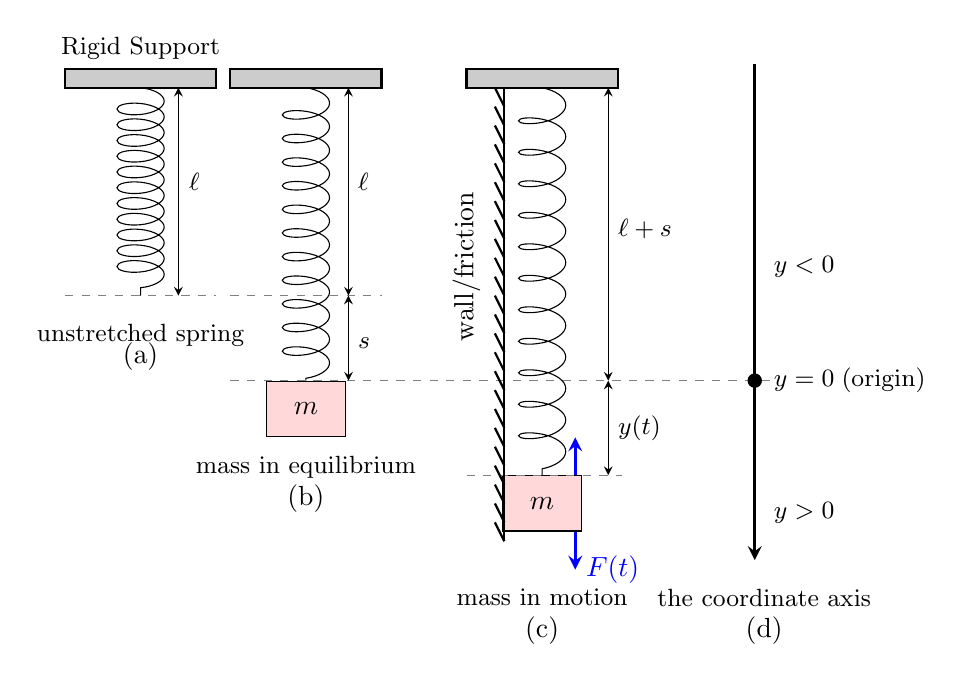
\begin{tikzpicture}[scale=1.2,>=stealth]
		\tikzset{
			spring/.style={thick,decorate,decoration={coil,aspect=0.4,segment length=4pt,amplitude=3pt}},
			mass/.style={draw,fill=pink!60,minimum width=1cm,minimum height=0.7cm},
			dashedline/.style={dashed,gray},
			labeltext/.style={font=\small}
		}
		%--------------------------------
		% (a) Unstretched spring
		%--------------------------------
		\begin{scope}[xshift=0cm]
			\node[below] at (0,-2.6) {(a)};
			% Ceiling
			\draw[thick,fill=gray!40] (-0.8,0) rectangle (0.8,0.2);
			\node[above] at (0,0.2) {\small Rigid Support};
			% Spring (natural length l)
		\draw[decoration={aspect=0.4, segment length=2mm, amplitude=3mm,coil},decorate] (0,0) -- (0,-2.2); 
			%\draw[spring, aspect=0.7] (0,0) -- (0,-2.2);
			\draw[<->] (0.4,0) -- (0.4,-2.2);
			\node[right,labeltext] at (0.41,-1) {$\ell$};
			% Dashed reference line
			\draw[dashedline] (-0.8,-2.2) -- (0.8,-2.2);
			\node[below,labeltext] at (0,-2.4) {unstretched spring};
		\end{scope}
		
		%--------------------------------
		% (b) Equilibrium position
		%--------------------------------
		\begin{scope}[xshift=1.75cm]
			\node[below] at (0,-4.1) {(b)};
			% Ceiling
			\draw[thick,fill=gray!40] (-0.8,0) rectangle (0.8,0.2);
			%\node[above] at (0,0.2) {\small Rigid Support};
			% Spring
			\draw[decoration={aspect=0.4, segment length=3mm, amplitude=3mm,coil},decorate] (0,0) -- (0,-3.1);
			%\draw[spring] (0,0) -- (0,-3.1);
			\node[mass] (m1) at (0,-3.4) {$m$};
			% Labels
			\draw[<->] (0.45,0) -- (0.45,-2.2);
			\node[right,labeltext] at (0.45,-1) {$\ell$};
			%\node[right,labeltext] at (0,-2.4) {$s$};
			\draw[dashedline] (-0.8,-3.1) -- (5,-3.1); %the line corresponding to the origin
			\draw[dashedline] (-0.8,-2.2) -- (0.8,-2.2);
			% Bracket for s
			\draw[<->] (0.45,-2.2) -- (0.45,-3.1);
			\node[right,labeltext] at (0.45,-2.7) {$s$};
			\node[below,labeltext] at (0,-3.8) {mass in equilibrium};
		\end{scope}
		
		%--------------------------------
		% (c) Motion (displacement x or y)
		%--------------------------------
		\begin{scope}[xshift=4.25cm]
			\node[below] at (0,-5.5) {(c)};
			% Ceiling
			\draw[thick,fill=gray!40] (-0.8,0) rectangle (0.8,0.2);
			%\node[above] at (0,0.2) {\small Rigid Support};
			% Spring
			\draw[decoration={aspect=0.4, segment length=4mm, amplitude=3mm,coil},decorate] (0,0) -- (0,-4.1);
			%\draw[spring] (0,0) -- (0,-3);
			\node[mass] (m2) at (0,-4.4) {$m$};
			% Labels
%			\node[right,labeltext] at (0,-1.3) {$\ell$};
%			\node[right,labeltext] at (0,-2.7) {$s$};
			
			% Bracket for total extension
			\draw[<->] (0.7,0) -- (0.7,-3.1);
			\node[right,labeltext] at (0.7,-1.5) {$\ell + s$};
	
			\draw[<->] (0.7,-4.1) -- (0.7,-3.1);
			\node[right,labeltext] at (0.7,-3.6) {$y(t)$};
			% Dashed lines
			%\draw[dashedline] (-0.8,-2.2) -- (0.8,-2.2);
			\draw[dashedline] (-0.8,-4.1) -- (0.85,-4.1);
			%\draw[dashedline] (-0.8,-4.7) -- (0.8,-4.7);
			\node[below,labeltext] at (0,-5.2) {mass in motion};
			
			% Thick vertical wall
			\draw[thick] (-0.4,-4.8) -- (-0.4,0);
			% Friction hatch marks (diagonal lines)
			\foreach \y in {-4.8,-4.6,...,-0.2}
			\draw[thick] (-0.4,\y) -- (-0.5,\y+0.2);
			
			
			% Optional label
			\node[rotate=90,left] at (-0.8,-1) {\text{wall/friction}};
			
%			% Example mass block next to wall
%			\draw[fill=gray!30] (0.5,1) rectangle (1.5,2);
			
			% Optional arrow to indicate external force
			\draw[->,blue,very thick] (0.35,-4.1) -- (0.35,-3.7) node[right] {};
			\draw[->,blue,very thick] (0.35,-4.7) -- (0.35,-5.1) node[right] {$F(t)$};
		\end{scope}
			%--------------------------------
		% (d) Coordinate system
		%--------------------------------
		\begin{scope}[xshift=3.5cm]
				\node[below] at (3.1,-5.5) {(d)};
			
			% Bracket for total extension
			\draw[->,very thick] (3,0.25) -- (3,-5); % the coordinate axis line
		
	
			\node[right,labeltext] at (3.1,-1.9) {$y<0$};
			
			\filldraw[black] (3,-3.1) circle (2pt); 
			\node[right,labeltext] at (3.1,-3.1) {$y=0$\;(origin)};
			\node[right,labeltext] at (3.1,-4.5) {$y>0$};
			% Dashed lines
			%\draw[dashedline] (-0.8,-2.2) -- (0.8,-2.2);
%			\draw[dashedline] (-0.8,-4.3) -- (0.8,-4.3);
%			\draw[dashedline] (-0.8,-4.7) -- (0.8,-4.7);
			\node[below,labeltext] at (3.1,-5.2) {the coordinate axis};
			%\node[below,labeltext] at (3.1,-5.1)  {positive downward};
	
		\end{scope}

	\end{tikzpicture}
\caption{}
\label{fig:mass-spring}
\end{figure}


Let \(\ell\) denote the natural (unstretched) length of the spring, and let \(s\) be the amount by which the spring stretches when the mass $m$ is attached and allowed to hang in equilibrium under gravity. We assume that the motion of the mass is restricted to the vertical line  through the point of the equilibrium  of the mass. To take this vertical line (see Figure~\ref{fig:mass-spring} (d)) as the coordinate axis, we take the equilibrium point as the origin and assign the vertically downward direction as the positive direction.



Denote by \(y(t)\) the displacement of the mass at time \(t\) from its equilibrium position (the origin). 
In addition to the restoring force \(F_{\text{s}}(t)\) of the spring and gravitational force $mg$, assume that the mass is acted upon by a damping force \(F_{\text{d}}(t)\) as well as an external force \(F(t).\) See  Figure~\ref{fig:mass-spring} (c) for wall friction as an example of a damping force.  Thus, we have
\[
\text{the net force on the mass} = F_{\text{s}}(t) +mg+  F_{\text{d}}(t) + F(t).
\]
According to Newton’s second law, we then have
\begin{equation}\label{eq:mass-spring1}
m y''(t) = F_{\text{s}}(t) + mg+ F_{\text{d}}(t) + F(t).
\end{equation}


 \noindent$\bullet$ How do we model the spring force $F_{\text{s}}(t)?$  
 
 Since a spring that is stretched or compressed tends to return to its natural length, the spring force  wants to pull the mass toward its equilibrium position. For an ideal spring—one made of a homogeneous material with uniform coiling—Robert Hooke, a 17th-century English physicist, established that the restoring force required to stretch or compress the spring (without damaging it) is directly proportional to the resulting displacement.\footnote[1]{ For a spring made up of a heterogeneous material and with nonuniform coiling, the restoring force may be modeled by a nonlinear function of  the displacement. For example, \( F_{\text{s}}(t) = - k\,\abs{y(t)}^{p-2}y(t)\) with $p$ a fixed number in \((1, \infty)\) and $k>0$  a fixed real number.} 
This means that 
\begin{equation}\label{eq:mass-spring2}
	 F_{\text{s}}(t) = - k\,(s+y(t)),
	 \end{equation}
where $k$ is a fixed positive constant, called the spring constant which measures the stiffness of the spring. The negative $(-)$ means that the restoring force is directed toward the origin. 

One may ask:  {\textit{how do we practically calculate $k$ of a spring?}} The simplest way to calculate $k$ is to simply suspend the spring from a support with the mass attached to its other end and observe the stretch $s$ the spring experiences for its equilibrium under gravity. Since the mass is at rest, the net force acting on the mass is zero, that is, 
\[\text{the net force on the mass}=0 = - ks +mg,\] which yields
\begin{equation}\label{eq:mass-spring3}
	mg = ks,
	\end{equation} and so
\[k = \frac{mg}{s}.\] 

 \noindent$\bullet$ How do we model $F_{\text{d}}(t)?$
 
It is intuitive that the damping force (or drag) increases as the speed of the mass increases. Hence, the simplest way to model the damping force is to assume that it is directly proportional to the velocity.\footnote[2]{For a medium that resists the motion of the mass  depending on a power of the speed,  the damping force may be modeled by a nonlinear function of  the velocity. For example, \( F_{\text{s}}(t) = - b\,\abs{y'(t)}^{q-2}y'(t)\) with $q$ a fixed number in \((1, \infty)\) and $b>0$ a fixed real number.}
This means that 
\begin{equation}\label{eq:mass-spring4}
F_{\text{d}}(t)=  - b\, y'(t), \end{equation}
where 
$b$ is the constant of proportionality, called the damping coefficient of the medium offering the resistance to the motion of the mass.

Using \eqref{eq:mass-spring2} and \eqref{eq:mass-spring4} in \eqref{eq:mass-spring1}, we obtain

\[
	m y''(t) = -ks -k y(t) + mg- b y'(t) + F(t),
\] which, in view of \eqref{eq:mass-spring3}, yields
\begin{equation}\label{eq:mass-spring5}
	my''(t) + by'(t) + k y(t) = F(t).
\end{equation}
This is a second order linear differential equation with constant coefficient, and it can be solved using the methods from the previous sections. For example, the method of undetermined coefficients or variation of parameters can be used.

We now examine several interesting and special cases of \eqref{eq:mass-spring5} before  discussing the general form. 
 

\subsubsection{I. Free Undamped Motion ($b=0,\;F(t) =0$)}	
  When $b= 0$ (no damping) and $F(t) = 0$ (no external forces), the mass-spring system is said to have  a free undamped motion and the system  is called a \textit{simple harmonic oscillator}.   The resulting differential equation for the displacement of the mass from its equilibrium position is 
	\[	my''(t)  + k y(t) = 0,\] which, with $w^2 = k/m$,  becomes
	\begin{equation}\label{eq:mass-spring6}
		y''(t) + \omega^2 y(t) = 0,
		\end{equation}
	also referred to as a simple harmonic oscillator.
	Then the general solution of the simple harmonic oscillator is 
	\begin{equation}\label{eq:mass-spring7}
		y(t) = c_1 \cos(\omega t) + c_2 \sin(\omega t),
		\end{equation} where $c_1$ and $c_2$ are arbitrary constants  which can be determined when the initial conditions $y(t_0) = y_0,  y'(t_0) = y_1$ are  provided.
	
		The displacement $y(t)$ described by \eqref{eq:mass-spring7} can  interpreted most effectively when it is written in the form of a single sine or cosine function. To express it in the form of a single sine function,
	we seek to find two constants $A$ and $\phi$ so that 
	\begin{equation}\label{eq:mass-spring8}
	y(t) = A \sin(\omega t -\phi).
	\end{equation}
	Then 
		\begin{equation}\label{eq:mass-spring9}
	y(t) = A \sin(\omega t) \cos(\phi) - A\cos(\omega t) \sin (\phi).\
\end{equation}
	Since the terms in \eqref{eq:mass-spring7} and \eqref{eq:mass-spring9} must match, we obtain
	\[\begin{cases}
		A\sin(\phi) = -c_1,\\
		A\cos(\phi) = c_2.
	\end{cases}
	\]
	Squaring and adding these equations gives $A^2 = c_1^2 + c_2^2.$  We take 
	$A =\sqrt{c_1^2 + c_2^2}.$ It is possible that $A =0$, in which case, we have $y(t) = 0$ for all $t$, the trivial solution, and this means that the mass is at rest in the equilibrium position for all $t.$ Therefore the only interesting case is when $A>0.$  
	If $c_2 \ne 0,$ then \[\arctan(\frac{-c_1}{c_2}) \text{ lies in }\left(-\frac{\pi}{2}, \frac{\pi}{2}\right). \]
 We have
	\[\phi = \begin{cases}
		\arctan(\frac{-c_1}{c_2}) &\text{if } c_2>0,\\[1em]
		\arctan(\frac{-c_1}{c_2})+\pi&\text{if } c_2<0,\\
		\frac{\pi}{2}&\text{if }c_1<0 \text{ and } c_2=0,\\
		-\frac{\pi}{2}&\text{if } c_1>0 \text{ and } c_2=0.
		\end{cases}
			\]
Also, note that \eqref{eq:mass-spring8} can be written as
\begin{equation}
	y(t) = A \cos(\omega t -\phi -\frac{\pi}{2}).
\end{equation}		
It is now clear from \eqref{eq:mass-spring8} that the mass oscillates about the origin with the amplitude  $A,$ which is the maximum displacement from the equilibrium position. The  time period for one complete oscillation is $ T= 2\pi / \omega,$ and therefore the number $\omega $ is  the circular frequency of the oscillations, that is, the number of cycles per unit $2\pi$ units of time.
	

\begin{example}
A 2-pound mass stretches a spring 6 inches. At time \( t = 0 \), the mass is released from a position 8 inches below equilibrium with an initial upward velocity of \( \tfrac{4}{3} \) ft/s. 
\begin{enumerate}[label =(\roman*), noitemsep]
	\item\label{item:1} Find the equation of motion in both the forms \eqref{eq:mass-spring7} and \eqref{eq:mass-spring8}.
	\item\label{item:2} Graph the velocity versus the displacement.
\end{enumerate}


\end{example}		

\begin{solution} 
	\ref{item:1} Let $y(t)$ denote in feet the displacement of the mass from the equilibrium position measured positively in the vertically downward direction. We have 
\(mg = 2~\text{lb}, 
	\text{spring stretch}, s = 6~\text{in} = 0.5~\text{ft}.
\)
We have
\(
m = \frac{mg}{g} = \frac{2}{32} = \frac{1}{16}~\text{slug},\) and 
the spring constant
\(k = \frac{mg}{s} = \frac{2}{0.5} = 4~\text{lb/ft}.
\)
The differential equation of motion is
\[
m y'' + k y = 0,\] which becomes
\[\frac{1}{16} y'' + 4y = 0,\] and therefore
\[y'' + 64y = 0.\]

with the initial condition $y(0) =  -\tfrac{2}{3}, 
y'(0) = \tfrac{4}{3}.$
The general solution of the differential equation is
\[y(t) = c_1 \cos(8t) + c_2 \sin(8t).
\]

Applying the initial conditions gives
\[
y(0)=  -\frac{2}{3} = c_1.\]
Also, since
\[y'(t) = -8c_1 \sin(8t) + 8c_2 \cos(8t)\]  and
\(y'(0) =\frac{4}{3},\)
we obtain 
\(8c_2 = \frac{4}{3},\) that is, 
\(
 c_2 = \frac{1}{6}.
\)
Hence the equation of the motion is
\[
	y(t) = -\frac{2}{3} \cos(8t) + \frac{1}{6} \sin(8t),
\]
which is of the form \eqref{eq:mass-spring7}.
Using the method discussed for \eqref{eq:mass-spring8} to find
 the equation of the motion in the amplitude-phase, we compute
 \[A= \sqrt{c_1^2+c_2^2}=\sqrt{\frac{4}{9}+\frac{1}{36}}= \frac{\sqrt{17}}{6} \]
  and
  \[ \phi = \arctan(\frac{-c_1}{c_2}) = \arctan(\frac{2/3}{1/6}) =\arctan(4)\approx 1.3258~\text{rad},\] and therefore
\[
y(t) = \frac{\sqrt{17}}{6} 
\sin\!\left(8t - \varphi\right)
\approx  \frac{\sqrt{17}}{6} 
\sin\!\left(8t - 1.3258\right).
\] Its graph is shown in Figure~\ref{graph:simple-harmonic-oscillator}.


%\textcolor{red}{open the figure below}
\begin{figure}[h]
	\centering
	\begin{tikzpicture}[scale=.8]
		\begin{axis}[
			width=10cm,
			height=7cm,
			axis lines=middle,
			xlabel={$t$},
			ylabel={$y(t)$},
			ylabel style={at={(axis description cs:0, -0.02)}, anchor =north},
			samples=300,
			domain=0:1,
			xtick={0,0.1,0.2,...,1.0},
			ytick={-1,-0.5,0,0.5,1},
			smooth,
			thick,
			y dir=reverse, 
			grid=both,
			minor tick num=1,
			]
			\addplot[blue, thick] {sqrt(17)/6 * sin(deg(8*x - 1.3258))};
			\addplot[black, thick, dashed] {sqrt(17)/6 * sin(deg(8*x))};
			\node[anchor=west, blue] at (axis cs:0.37,.5) 
			{$y(t)=\dfrac{\sqrt{17}}{6}\sin(8t - \varphi)$};
				\node[anchor=west, black] at (axis cs:0.15,-0.3) 
			{$y(t)=\dfrac{\sqrt{17}}{6}\sin(8t)$};
		\end{axis}
	\end{tikzpicture}\\[1em]
	\caption{The graph of \(y(t) 
		\approx  \frac{\sqrt{17}}{6} 
		\sin\!\left(8t - 1.3258\right)\)}
	\label{graph:simple-harmonic-oscillator}
	\end{figure}
	
 \ref{item:2} We find \[y'(t) =  8\frac{\sqrt{17}}{6}
 \cos\!\left(8t - \varphi\right).\] Then
 \[\left(\frac{y(t)}{\frac{\sqrt{17}}{6} }\right)^2+\left(\frac{y'(t)}{\frac{8\sqrt{17}}{6}}\right)^2 = 1\] for all $t$. This takes the form 
 \[272 (y(t))^2 + 17(y'(t))^2= 272 \] for all $t$ and is an ellipse in the $y'y$-plane as shown in Figure~\ref{fig:phase-space-orbit}.  The graph is called the orbit of the simple harmonic oscillator and visualizes the oscillatory motion.
 
	

%\textcolor{red}{open the figure below}
\begin{figure}[h]
\centering	
			\begin{tikzpicture}[scale=.8]
				\begin{axis}[
					width=12cm,
					height=8cm,
					axis lines=middle,
					xlabel={$y'(t)$},
					ylabel style={rotate=-90},
					%ylabel={$y(t)$},
					%ylabel style={at={(axis description cs:.0, 1)}, anchor =north},
					grid=none,
					minor tick num=1,
					samples=400,
					domain=0:2*pi,
					axis equal image,  % keeps scaling equal after manual adjustment
					thick,
					y dir=reverse,     % make y(t) axis point downward
					x dir=normal,
					xscale=1,
					yscale=3,
					xmin=-6.5, xmax=6.5,               % explicit limits prevent huge dimensions
					ymin=-1.1, ymax=1.1,     % scale horizontal axis by 1/8 (since y' = 8A cos)
					]
					
					% Parameters: A = sqrt(17)/6, omega = 8, phi = 1.3258
					
				
					\addplot[
					blue,
					thick,
					smooth,
					postaction={decorate, decoration={markings,
							mark=between positions 0.05 and 0.95 step 0.1 with {\arrow{stealth};}
					}}
					] (
					{8*sqrt(17)/6 * cos(deg(8*x - 1.3258))},   % x = y'(t)
					{sqrt(17)/6 * sin(deg(8*x - 1.3258))}      % y = y(t)
					);
					
				% Initial point (inside axis limits)
				\addplot[only marks, mark=*, mark options={fill=red, scale=.7}] coordinates {(4/3,-2/3)};
				\node[above right, red] at (axis cs:.1,-0.7) {$(y'(0),y(0)) = (4/3, -2/3)$};
				
				% Key points (placed within axis limits)
				\addplot[only marks, mark=*, mark options={fill=black, scale=.7}] coordinates {(0,2/3) (0,-2/3) (16/3+.19,0) (-16/3-.19,0)};
				\node[right]       at (axis cs: 0, 1)  {{$y(t)$}};

		
				\end{axis}
			\end{tikzpicture}\\[1em]
			\caption{The orbit of  $y''+64y = 0, y'(0)= -2/3, y'(0) = 4/3.$}
			\label{fig:phase-space-orbit}
\end{figure}
\end{solution}		

	
\subsubsection{II. Free Damped Motion
	($b>0, \;F(t) = 0)$} 
	When $b> 0$ (with damping) and $F(t) = 0$ (no external forces), the mass-spring system is said to have a \textit{free damped motion}. The resulting differential equation for the motion of the mass is 
	\[	my''(t)+by'(t) + k y(t) = 0,\] which, with $2\beta = \frac{b}{m}$ and $w^2 = \frac{k}{m}$,  becomes
	\begin{equation}\label{eq:mass-spring10}
		y'' + 2\beta y'+ \omega^2 y = 0,
	\end{equation}
	and 
the differential equation \eqref{eq:mass-spring10} is known as a \textit{free damped spring–mass system.} Its general solution depends on the relative strengths of the damping and spring forces. When the spring force dominates, the motion is oscillatory with amplitude decaying to zero  as \( t \to \infty \) and when the damping force dominates, the motion is non-oscillatory. There exists a threshold value of the damping coefficient—called the critical damping—above which no oscillations occurs, and below which the system exhibits damped oscillations whose amplitude decays to zero as \( t \to \infty \). To analyze this, we start with the auxiliary equation for \eqref{eq:mass-spring10}; namely,
\[r^2 + 2\beta r + \omega ^2 =0,\] with $y(t)=e^{rt}$ is a trial solution. It then follows that 
\begin{equation}\label{eq:mass-spring11}
	r = \frac{-2\beta\pm\sqrt{4\beta^2 - 4 \omega^2}}{2} = -\beta\pm\sqrt{\beta^2 -  \omega^2}. \end{equation}
	
There are three significantly different cases of a free damped motion. 
\begin{enumerate}[leftmargin=1.5em,label = (\arabic*)]
	\item\label{item:damping2}\textbf{\textit{Underdamped Motion}:}  When $\beta <\omega,$  \eqref{eq:mass-spring11} yields  \[r = - \beta \pm i \sqrt{\omega^2- \beta^2},\] so that the general solution of \eqref{eq:mass-spring10} is
	\[y(t) =  e^{-\beta t}\left(c_1\cos(\sqrt{\omega^2- \beta^2}\; t)+ c_2 \sin(\sqrt{\omega^2- \beta^2}\; t)\right),\] where $c_1$ and $c_2$ are arbitrary constants are determined when the initial conditions $y(t_0) = y_0,  y'(t_0) = y_1$ are provided.  
	The displacement $y(t)$ is periodic with the period $ 2\pi/\sqrt{\omega^2- \beta^2}.$  Moreover, 
	since $\beta >0,$ we observe that  \[\lim\limits_{t\to\infty} e^{-\beta t}\cos(\sqrt{\omega^2- \beta^2}\; t)=0 \quad \mbox{and} \quad \lim\limits_{t\to\infty}e^{-\beta t}\sin(\sqrt{\omega^2- \beta^2}\; t)=0.\]
	It then follows that 
	\[\lim\limits_{t\to\infty} y(t)=0.\] 
	
	
	With regard to the velocity of the mass, we find
		\[\begin{split}
	y'(t) &= -\beta e^{-\beta t}\left(c_1\cos(\sqrt{\omega^2- \beta^2}\; t)+ c_2 \sin(\sqrt{\omega^2- \beta^2}\; t)\right)\\
	& + \sqrt{\omega^2- \beta^2}e^{-\beta t}\left(-c_1\sin (\sqrt{\omega^2- \beta^2}\; t)+ c_2 \sin(\sqrt{\omega^2- \beta^2}\; t)\right).
	\end{split}
	\]
	Again, we observe that
	\[\lim\limits_{t\to\infty} y'(t)=0.\]  Hence, the mass approaches the equilibrium position while oscillating with the circular frequency \(\sqrt{\omega^2- \beta^2}\) and the velocity approaches zero as $t$ goes to $\infty.$
	
	Since $\beta = b/(2m)$ and $\omega^2 = k/m,$ $\beta < \omega$ is equivalent to $b< 2\sqrt{mk}.$ 
	We conclude that when the damping force is too weak to counteract a strong spring force, the mass undergoes damped oscillations: the amplitude  gradually decreases to zero. In this case, the mass-spring system is said to be \textbf{\textit{underdamped}}.\index{spring-mass systems!underdamped}
	
	
	\item\label{item:damping3}\textbf{\textit{Overdamped Motion}:}  
	When $\beta >\omega,$  \eqref{eq:mass-spring11} yields  $r = - \beta \pm  \sqrt{\beta^2- \omega^2},$ so that the general solution of \eqref{eq:mass-spring10} is
	\[y(t) =  c_1e^{(-\beta + \sqrt{\beta^2- \omega^2})t}+ c_2e^{(-\beta - \sqrt{\beta^2- \omega^2})t},\] where $c_1$ and $c_2$ are arbitrary constants are determined when the initial conditions $y(t_0) = y_0,  y'(t_0) = y_1$ are provided.  
	Therefore $y(t)$ is not periodic   Moreover, 
	since $\beta >0$ and \(0<\sqrt{\beta^2- \omega^2} < \beta\),  it follows that both 
	\(-\beta + \sqrt{\beta^2- \omega^2}\) and 	\(-\beta - \sqrt{\beta^2- \omega^2}\) are negative.
	Consequently,
	  we have  \[\lim\limits_{t\to\infty} e^{(-\beta + \sqrt{\beta^2- \omega^2})t}=0 \quad \mbox{and} \quad \lim\limits_{t\to\infty}e^{(-\beta - \sqrt{\beta^2- \omega^2})t}=0.\]
	It then follows that \[\lim\limits_{t\to\infty} y(t)=0.\]  We can show that the mass passes through the equilibrium position at most once by setting $y(t) = 0$ and finding the time $t$ at which this happens.

Regarding the velocity of the mass, we find
	\[\begin{split}
		y'(t) &=  c_1 (-\beta + \sqrt{\beta^2- \omega^2})e^{(-\beta + \sqrt{\beta^2- \omega^2})t}\\
		&+ c_2(-\beta - \sqrt{\beta^2- \omega^2}) e^{(-\beta - \sqrt{\beta^2- \omega^2})t},
	\end{split}
	\]

	Again, we observe that
	\[\lim\limits_{t\to\infty} y'(t)=0.\]  
   We can also show that the mass reaches  an extreme position  at most once by setting $y'(t) = 0$ and finding the time $t$ at which this happens.\\
   
	Since $\beta = b/(2m)$ and $\omega^2 = k/m,$ $\beta > \omega$ is equivalent to $b> 2\sqrt{mk}.$ 
	We conclude that when the spring force is too weak to counteract a strong damping damping force, the mass  approaches the equilibrium position with no oscillation and its velocity approaches zero, by changing its sign at most once, as $t$ goes to $\infty$.  In this case, the mass-spring system is said to be \textbf{\textit{overdamped.}}\index{spring-mass systems!overdamped}
	
	
\item\label{item:damping1} \textbf{\textit{Critically Damped Motion}:} 
	When $\beta = \omega$,
	 \eqref{eq:mass-spring11} yields  $r = - \beta, -\beta,$ so that the general solution of \eqref{eq:mass-spring10} is
	\[y(t) = c_1 e^{-\beta t}+ c_2 te^{-\beta t} = (c_1+ c_2t) e^{-\beta t},\] where $c_1$ and $c_2$ are arbitrary constants  which can be determined when the initial conditions $y(t_0) = y_0,  y'(t_0) = y_1$ are known.  The velocity of the mass is given by 
	\[y'(t) = -\beta (c_1 + tc_2) e^{-\beta t} + c_2 e^{-\beta t} = (c_2 - \beta c_1- \beta c_2 t) e^{-\beta t}.\]  Since $\beta >0,$ we find $e^{-\beta t}\to 0$ and $t e^{-\beta t}\to 0$ as $t\to\infty.$  These imply that 
	\[\lim\limits_{t\to\infty} y(t) = 0 \qquad \mbox{ and }\qquad \lim\limits_{t\to\infty} y'(t) = 0.\]
As note earlier in the case of an overdamped motion, the mass in this case can also pass thorough the equilibrium at most once and can reach an extreme position at most once while its velocity changes its sign.  As $t$ goes to $\infty,$ the mass approaches its equilibrium position and its velocity also tends to zero.

\medskip Since $\beta = b/(2m)$ and $\omega^2 = k/m,$ $\beta = \omega$ is equivalent to  $b= 2\sqrt{mk}.$ It follows
from the case of underdamped motion  that when the damping coefficient $b$ is even slightly less than  $2\sqrt{mk},$ the mass undergoes  an oscillatory motion. The spring-mass system with the smallest damping  coefficient  $b$ that maintains a nonoscillatory motion is  to be \textbf{\textit{critically damped}}.\index{spring-mass systems!critically damped}
\end{enumerate}	

\subsubsection{III. Undamped and Forced Motion ($b=0, \; F(t) \ne 0$)}
When $b=0$ (no damping) and $F(t) \ne 0$ (with external force), the spring-mass system is governed by the differential equation
\begin{equation*}
	my''(t)  + ky(t) = F(t).
\end{equation*}
 which, with $w^2 = k/m$ and $f(t) = F(t)/m,$  becomes
 \begin{equation}\label{eq:mass-spring-undamped-forced-1}
 	y''(t)  + \omega^2y(t) = f(t).
 \end{equation}
 
The nonhomogeneous equation \eqref{eq:mass-spring-undamped-forced-1} can be solved by using the methods of previous sections. The general solution  is of the form
\begin{equation}\label{eq:mass-spring13}
	y(t) = y_h(t) + y_p(t) = c_1 \cos(\omega t) + c_2 \sin(\omega t) +y_p(t),
\end{equation}
where $c_1$ and $c_2$ are arbitrary constants and $y_p(t)$ is a particular solution of \eqref{eq:mass-spring-undamped-forced-1}. Recall that 
 \[y_h(t) = c_1 \cos(\omega t) + c_2 \sin(\omega t) \] is the general solution of the  simple harmonic oscillator \[ y''(t)  + \omega^2 y(t)=0,\]  associated with  \eqref{eq:mass-spring-undamped-forced-1}. 

\begin{example}[\(b=0, F(t)= F_0 \sin(\gamma t)\)]\label{eg:undamped-forced-system}
	A \(10\)-kilogram mass attached to the  end of a vertically hanging spring causes the spring to stretch \(39.2\) centimeters. At time \( t = 0 \), the mass–spring system is set into motion by an external force \( F(t) = 180\sin(10t) \), where \( F(t) \) is measured in newtons and is positive in the downward direction, and time is measured in seconds. Determine the equation of motion and estimate the maximum excursion of the mass from its equilibrium position.  
\end{example}

 \begin{solution}
 We have
 \(
 m = 10~\text{kg},  
 s = 39.2~\text{cm} = 0.392~\text{m},  
 F(t) = 180\sin(10t)~\text{N}.
 \)
 For the mass in equilibrium, we have \( mg = ks \), and so
 \[
 k = \frac{mg}{s} = \frac{10 \times 9.8}{0.392} = 250~\text{N/m}.
 \]
 The natural  frequency of the system is
 \[
 \omega = \sqrt{\frac{k}{m}} = 5 \text{ cycles in $2\pi$ seconds} = 5 \text{ rad/s}
 \]
 The differential equation of motion is therefore
 \[
 10y'' + 250y' = 180\sin(10t),
 \]
 or equivalently,
 \begin{equation}\label{eq:mass-spring-150}
 	y'' + 25y = 18\sin(5t). 
 \end{equation}
 The general solution of \( y'' + 25y = 0 \) is
 \[
 y_h(t) = c_1\cos(5t) + c_2\sin(5t),
 \]
 where $c_1$ and $c_2$ are arbitrary constants.
 We find a particular solution $y_p(t)$ of \eqref{eq:mass-spring-150} by variation of parameters.
 Let
 \[
 y_p(t) = A\cos(10t) + B\sin(10t)
 \]
be a particular solution of \ref{eq:mass-spring-150}, where $A$ and $B$ are to be determined.
We find that $y''_p(t) = - 100 y_p(t).$ Substituting $y_p$  for $y$ and $y''_p$ for $y''$  into \eqref{eq:mass-spring-15}   yields
\[- 100 y_p(t)+25y_p(t) = 18 \sin(10t),\]
that is,
\[-75A \cos(5t) - 75 B\sin(5t) =18 \sin(10t).\]
Equating the coefficients of the like terms, we have
\(-75 A =0\) and \(-75 B = 18\), that is, $A=0$ and $B = -6/25.$
Thus, we have 
\[ y_p(t) = -\frac{6}{25} \sin(5t).\]
 The general solution of \ref{eq:mass-spring-15} is 
 \[
 y(t) = c_1\cos(5t) + c_2\sin(5t) - \frac{6}{25}\sin(10t),
 \]
 where $c_1$ and $c_2$ are arbitrary constants. The initial conditions for $y(t)$ are  $y(0) = 0, y'(0) = 0.$
 Substituting these gives \( c_1 = 0 \) and \( 5c_2 - \frac{12}{5} = 0\), i.e.,  \(c_1=0\) and \(c_2 = \frac{12}{25} \)
 Thus, we have
 \[
 y(t) = \frac{12}{25}\sin(5t) - \frac{6}{25} \sin(10t).
 \] The graph of the solution is shown in Figure~\ref{fig:undamped-forced-system}.
 Using the critical numbers and second derivative test, we can verify that the maximum occurs at $t = \frac{2\pi}{15}.$ The maximum value is 
 \[y\left(\frac{2\pi}{15}\right) = \frac{9\sqrt{3}}{25} \approx 0.6235.\qedhere\]
 
 %\textcolor{red}{open the figure below}
\begin{figure}[H]
	\centering
	\includegraphics[width=0.5\linewidth]{chap03/mathematica/undamped-forced-system}
	\caption{The graph of \(y(t) = \frac{12}{25} \sin(5t)-\frac{6}{25}\sin(10t)\)}
	\label{fig:undamped-forced-system}
\end{figure}
 \end{solution}
In Example~\ref{eg:undamped-forced-system},  the frequency of the external source is $\gamma =10$ which is not equal to  or near the natural frequency $\omega = 5.$  

\textbf{Resonance:}\index{resonance} An important aspect of analyzing undamped  forced spring-mass systems is understanding how large (in absolute values) the values of $y_p(t)$ can become  when $F(t)$ is  sinusoidal. If the amplitude of $y_p(t)$ grows without bound,  the system is said to be in \textbf{\textit{resonance}}. In practical applications,  resonance may be undesirable because it can lead to excessive energy buildup and potential system failure. Since the system \eqref{eq:mass-spring-undamped-forced-1} is undamped, the only way energy can dissipate from the system is by the nature of the source term $F(t).$ However, it is possible that the energy  buildup can happen in the system even when $F(t)$ is sign-changing. The following example demonstrates how resonance occurs.


 
\begin{example}[Resonance: $b=0, F(t)= F_0 \sin(\omega t)$]\label{eg:resonance-mass-spring-1}
With the external force in Example~\ref{eg:undamped-forced-system} replaced with  \( F(t) = 180\sin(5t)\),  determine the equation of motion, analyze the amplitude of the resulting motion, and verify that the system exhibits resonance.
\end{example}
\begin{solution} Similarly to the solution in Example~\ref{eg:undamped-forced-system}, the initial value problem for the current example is
	\begin{equation} \label{eq:mass-spring-15}
		y'' + 25y = 18\sin(5t), \quad y(0) =0,\; y'(0) = 0.
	\end{equation}
	Recall from Example~\ref{eg:undamped-forced-system} that the natural  frequency of the system is
	\(
	\omega  = 10.
	\)
	We note here that the frequency of the external force $\gamma =10$ matches the natural frequency $\omega = 10.$
	The general solution of \( y'' + 25y = 0 \) is
	\[
	y_h(t) = c_1\cos(5t) + c_2\sin(5t),
	\]
	where $c_1$ and $c_2$ are arbitrary constants.
	We find a particular solution $y_p(t)$ of \eqref{eq:mass-spring-15} by variation of parameters.
	Let
	\[
	y_p(t) = u_1(t)\cos(5t) + u_2(t)\sin(5t),
	\]
	where \( u_1'(t) \) and \( u_2'(t) \) satisfy
	\[
	\begin{cases}
		u_1'(t)\cos(5t) + u_2'(t)\sin(5t) = 0, \\[4pt]
		-5\,u_1'(t)\sin(5t) + 5u_2'(t)\cos(5t) = 18\sin(5t).
	\end{cases}
	\]
	Solving this system gives
	\[
	u_1'(t) = -\frac{18}{5}\sin^2(5t) =-\frac{9}{5}(1-\cos(10t)),\] and  
	\[u_2'(t) = \frac{18}{5}\sin(5t)\cos(5t) =\frac{9}{5}\sin(10t).
	\]
	Integrating yields
	\[
	u_1(t) = -\frac{9}{5}t + \frac{9}{50} \sin(10t), \qquad 
	u_2(t) = -\frac{9}{50} \cos(10t).
	\]
	Hence,
	\[
	\begin{aligned}
		y_p(t) &= u_1\cos(5t) + u_2\sin(5t) \\[2pt]
		&= -\frac{9}{5}t \cos(5t)  + \frac{9}{50}\sin(10t) \cos(5t) 
		-\frac{9}{50}\cos(10t)\sin(5t)\\[2pt]
		&=-\frac{9}{5}t \cos(5t)  + \frac{9}{50}\sin(5t). \\[2pt]
	\end{aligned}
	\]
%	The dominant (secular) term responsible for resonance is
%	\[
%	y_p^{(\text{secular})} = -\frac{9}{10} t\cos(10t).
%	\]
%	
%	---
The general solution  is 
	\[
	y(t) = c_1\cos(5t) + c_2\sin(5t) - \frac{9}{5}t\cos(10t),
	\]
	$c_1$ and $c_2$ are constants to be determined so that  $y(0) = 0, y'(0) = 0.$
	Substituting these gives \( c_1 = 0 \) and \( 5c_2 - \frac{9}{5} = 0\), i.e.,  \(c_2 = \frac{9}{25} \)
Thus, we have
	\[
	y(t) = -\frac{9}{5}t\cos(5t) + \frac{9}{25}\sin(5t).
	\]
	It is evident  that the amplitude $a(t)$ of \(y(t)\) is given by \[a(t)=\frac{ 9}{5}\sqrt{t^2+\frac{1}{25}}\] which shows  that $\abs{y(t)}$ grows without bound as $t\to\infty.$ Hence,  the system exhibits \textbf{resonance} in this case, where the forcing frequency coincides the natural frequency--illustrating the classical example of resonance in an undamped forced spring--mass system. The plots of the solution $y(t)$ and amplitude $a(t)$ are shown in Figure~\ref{fig:resonance-1}.
	
%	\textcolor{red}{open the figure below}
\begin{figure}[h]
	\centering
	\includegraphics[width=0.9\linewidth]{chap03/mathematica/resonance-1}
	\caption{}
	%The graphs of $y(t) = -\frac{9}{10}t\cos(10t) + \frac{9}{100}\sin(10t)$\\ and its amplitude $a(t)=\frac{ 9}{10}\sqrt{t^2+\frac{1}{100}}$. 
	\label{fig:resonance-1}
\end{figure}
\end{solution}




\subsubsection{IV. Damped and Forced Motion ($b>0,\; F(t) \ne 0$)}
 When $b>0$ and $F(t) \ne 0$, the spring-mass system  is governed by the differential equation \eqref{eq:mass-spring6}; namely,
\begin{equation}\label{eq:mass-spring16}
	my''(t) + by'(t) + k y(t) = F(t).
\end{equation}
The nonhomogeneous equation \eqref{eq:mass-spring16} can be solved by using the methods of previous sections. The general solution is of the form
\begin{equation}\label{eq:mass-spring17}
	y(t) = y_h(t) + y_p(t),
\end{equation}
where $y_h(t)$ is the general solution of the  homogeneous equation \[ my''(t) + by'(t) + k y(t)=0,\] which describes the free damped motion corresponding to $F(t) = 0$ and $y_p(t)$ is a particular solution of \eqref{eq:mass-spring16}.  We recall from all three cases (underdamped,  critically damped, and overdamped) of a free damped motion that
\begin{equation}\label{eq:mass-spring18}
	\lim\limits_{t\to\infty}y_h(t) =0,
\end{equation}
and therefore $y_h(t)$ is  a \textbf{\textit{transient term}} in \eqref{eq:mass-spring17} and it is either oscillatory or nonoscillatory according as $b<2\sqrt{mk}$ or $b \ge \sqrt{mk}.$ We conclude from \eqref{eq:mass-spring17} and \eqref{eq:mass-spring18}  that 
\[y(t)\approx  y_p(t)\quad \mbox{ for large } t.\]
The particular solution $y_p(t)$ is called the \textbf{\textit{steady-state}} solution of \eqref{eq:mass-spring16}. For short times,  $y_h(t)$ must be included in the solution  $y(t) = y_h(t) + y_p(t),$ which then becomes  the \textit{\textbf{transient solution.}}


%\textcolor{red}{Even for a non-sinusoidal $F(t)$ in an overdamped system, we like to avoid situations when $y_p(t)$ assumes unexpectedly large values, as illustrated in an example to follow.}


\begin{example}[From Resonance to a Simple Harmonic Oscillator]\label{eg:resonance-mass-spring-4}
	For the resonant system  in Example~\ref{eg:resonance-mass-spring-1}, determine the  damping coefficient that should be introduced at \(t = 3\pi \) so that the system transitions immediately into  a simple harmonic oscillator with the amplitude $27\pi/5.$ 
\end{example}
\begin{solution}
	We recall that the solution of the resonant system in Example~\ref{eg:resonance-mass-spring-1}
		\begin{equation}\label{eq:resonance-mass-spring-2}
	\begin{cases}
		y'' +25 y = 18 \sin(5 t),\\
	y(0) =0, \quad y'(0) = 0,
	\end{cases}
	\end{equation}
  is
		\[
	y(t) = -\frac{9}{5}t\cos(5t) + \frac{9}{25}\sin(5t). 
	\]
	We observe that  $y(3\pi) = {27\pi}/{5}$ and $y'(3\pi)=0.$
	
	We now proceed to find the damping coefficient $b>0$ required to turn the resonant system ~\ref{eq:resonance-mass-spring-2}  into a simple harmonic oscillator starting at $t=3\pi$  with the  frequency of oscillation same as the natural frequency of resonant system and the amplitude $27\pi/5.$
We consider the initial value problem
	\begin{equation}\label{eq:resonance-mass-spring-6}
	\begin{cases}
		10y''+by' +250 y = 180 \sin(5t),\\
		y(3\pi)  ={27\pi}/{5}, \quad y'(3\pi)  = 0.
	\end{cases}
	\end{equation}
It is evident that for small $b>0$ the complementary function should be oscillatory. Suppose then that $b^2< 40000$ and put 
\[d = \frac{1}{20}\sqrt{10000-b^2}.\]
Then the general solution of the differential equation  in \eqref{eq:resonance-mass-spring-6}   can be written in the form
\[ y(t) =e^{-\frac{b}{20}(t-3\pi)} \Big(c_1 \cos\big(d(t-3\pi)\big)+c_2 \sin\big(d(t-3\pi)\big)\Big)-\frac{36}{b} \cos (5 t)\]	
where $c_1$ and $c_2$ are arbitrary constants.  The only way this represents the solution to a harmonic oscillator is when its transient term is zero which happens only when $c_1=c_2= 0$ because of the linear independence of $\cos\big(d (t-3\pi)\big)$ and $\sin\big(d (t-3\pi)\big).$ 
Since $y(3\pi) = 27\pi/5,$ we have
\[\frac{27\pi}{5}  = c_1 +\frac{36}{b}.\] In order that $c_1=0,$ we must have \[b= \frac{20}{3\pi}.\]
The condition $y'(3\pi) = 0$ ensures that $c_2=0$ because
\[0 =y'(3\pi)= -\frac{b}{20} c_1 +dc_2,\] which gives
\[c_2 = \frac{b}{20d} c_1 =0.\]
Thus, the damped  system introduced at $t  = 3\pi$ is 
\begin{equation}\label{eq:resonance-mass-spring-7}
	\begin{cases}
		10y''+\frac{20}{3\pi}y' +250 y = 180 \sin(5 t),\\
		y(3\pi)  ={27\pi}/{5}, \quad y'(3\pi)  = 0,
	\end{cases}
\end{equation}
with the solution 
\[z(t) = -\frac{27\pi}{5} \cos (5 t)\] for all $t\ge 3\pi.$ The problem \eqref{eq:resonance-mass-spring-7} is equivalent to the simple harmonic oscillator described by 
\begin{equation}\label{eq:resonance-mass-spring-8}
		\begin{cases}
			y''+25 y = 0,\\
			y(3\pi)  ={27\pi}/{5}, \quad y'(3\pi)  = 0.
		\end{cases}
	\end{equation}
This harmonic oscillator has  frequency same  as the natural frequency of the resonant system \eqref{eq:resonance-mass-spring-2} and  amplitude equal to $27\pi/5.$ The solution of the resonant system for $0\le t\le 3\pi$ and  its continuous transition to a damped forced system that exhibits the simple harmonic oscillator \eqref{eq:resonance-mass-spring-8}   for $t\ge 3\pi$ is 
\[y(t) = \begin{cases}
	-\frac{9}{5}t\cos(5t) + \frac{9}{25}\sin(5t) &\text{ for } 0
	\le t\le3\pi\\
	\frac{-27\pi }{5}  \cos (5 t) &\text{ for }  t\ge 3\pi.
\end{cases}
\]
The graph of this solution is shown in  Figure~\ref{fig:resonance-to-sho}.

%\textcolor{red}{open the figure below}
\begin{figure}[h]
	\centering
	\includegraphics[width=0.5\linewidth]{chap03/mathematica/resonance-to-sho}
	\caption{}
	\label{fig:resonance-to-sho}.
\end{figure}
\end{solution}

When \(b = 0\) and the natural frequency of the system matches that of an external sinusoidal force, as illustrated in Example~\ref{eg:resonance-mass-spring-1}, the system exhibits resonance. In contrast, we  recall that a free damped system  approaches its equilibrium as \(t \to \infty\). In most practical applications, the damping constant \(b\) is relatively small. Interestingly, when \(b > 0\) but  small, although the amplitude of the particular solution $y_p$ is not unbounded as $t\to \infty$,  the system displays a behavior approaching resonance because the damping is insufficient to suppress  large oscillations. Therefore $\gamma = \omega$ should be avoided even for small damping. The following example illustrates this phenomenon.


\begin{example}[$b\approx 0, F(t)= F_0 \sin(\omega t)$]\label{eg:resonance-mass-spring-5}
	In the resonant system discussed in Example~\ref{eg:resonance-mass-spring-1}, 
 suppose that the surrounding medium offers a damping force that is numerically equal to 0.01 times the instantaneous velocity. Find the equation of the motion and analyze the danger of having a low value of the damping coefficient.
\end{example}
\begin{solution}
	The initial value problem is
	\begin{equation}\label{eq:small-damping-1}
		\begin{cases}
			y''+0.001y' +25 y = 18 \sin(5 t),\\
			y(0)  =0, \quad y'(0)  = 0.
		\end{cases}
		\end{equation}
		The auxiliary equation for \(y''+0.001y' +25 y=0\) is
		\[r^2 +0.001 r + 25 =0 \] with solutions $r = -a\pm ib$, where 
		$a = 0.0005$ and $b = \frac{1}{2}\sqrt{100-10^{-6}}.$
Then the general solution of the homogeneous differential equation 
\[y_h(t) = e^{-at}\left(c_1 \cos(bt) + c_2 \sin(bt)\right),\] where $c_1$ and $c_2$ are arbitrary constants. Let $y_p(t) = A\cos(5t) + B\sin(5t)$ be  particular solution of the nonhomogeneous equation in \eqref{eq:small-damping-1}. Then
\[y'_p(t) = -5A\sin(5t) + 5B\cos(5t)\] and \[y''_p(t) = -25A\cos(5t) - 25B\sin(5t) = -25 y_p(t).\] Substituting $y_p$ for $y$ in the nonhomogeneous equation yields
\[-25 y_p(t)-0.005A \sin(5t)+0.005B\cos(5t) + 25y_p(t) =18 \sin(5 t), \] which gives $A = -3600$ and $B=0.$ Then $y_p(t) = -3600 \cos(5t)$, and therefore the general solution of the nonhomogeneous equation is
\[y(t) =  e^{-at}\left(c_1 \cos(bt) + c_2 \sin(bt)\right)- 3600 \cos(5t).\]
Since $y(0) = 0$, we have $0 = c_1 - 3600,$ i.e., $c_1 = 3600.$ Also, since $y'(0) = 0,$ we have 
$0 = -a c_1 +bc_2,$ which gives $c_2 = ac_1/b = 3600a/b.$ Thus, the solution to the initial value problem is 
\[y(t) = 3600 e^{-at}\left( \cos(bt) + \frac{a}{b} \sin(bt)\right)- 3600 \cos(5t).\] The graph of the solution is shown in Figure~\ref{fig:small-damping-0} over $[0, 20]$  shows that the system appears to have resonance-like behavior as in Figure~\ref{fig:resonance-1}. However,
it is evident that $y(t) \approx - 3600 \cos(5t)$ for large values of $t$. In particular, $y\left(7001\pi\right) \approx 3600.$

%\textcolor{red}{open the figure below}
\begin{figure}[h]
	\centering
	\includegraphics[width=0.5\linewidth]{chap03/mathematica/small-damping}
	\caption{The graph of \(y(t) =  3600 e^{-at}\left(\cos(bt) + \frac{3600a}{b} \sin(bt)\right)- 3600  \cos(5t).\) }
	\label{fig:small-damping-0}
\end{figure}
\end{solution}

In the following example, we examine an undamped forced system in which  the frequency of the external force is  slightly different from the natural frequency.


\begin{example}[$b=0, F(t)= F_0 \cos(\gamma t)$ with $\gamma \approx \omega$]\label{eg:resonance-mass-spring-6}
	In the setting of the resonant problem in Example~\ref{eg:resonance-mass-spring-1}, 
let us take the external force  $F(t) = 180 \cos(5t+2\epsilon t)$, where $\epsilon$ is very small.  Find the equation of the motion.
\end{example}

\begin{solution}
	The initial value problem  is
	\begin{equation}\label{eq:small-change-frequency-2}
		\begin{cases}
			y'' +25 y = 18 \cos(\gamma t),\\
			y(0)  =0, \quad y'(0)  = 0,
		\end{cases}
	\end{equation}
	where $\gamma =5+2\epsilon$ with $\epsilon$ a small nonzero number. We have thus considered the frequency of the external force close to the natural frequency. The general solution of $y''+25y =0$ is 
	\[y_h(t) = c_1 \cos(5t) + c_2 \sin(5t),\] where $c_1$ and $c_2$ are arbitrary constants.
	
	 Let $y_p(t) = A\cos(\gamma t) + B\sin(\gamma t)$ be a particular solution of the nonhomogeneous equation in \eqref{eq:small-damping-1}. Substituting $y_p$ for $y$ and $y''_p$ for $y''$ into the nonhomogeneous equation in \eqref{eq:small-change-frequency-2} gives
	\[(25-\gamma^2) A \cos(\gamma t) + (25-\gamma^2) B \sin(\gamma t) 
	= 18 \cos(\gamma t).\] This  gives
	\[ A = -\frac{18}{\gamma^2 -25} \quad\mbox{and}\quad B=0.\] Thus,
	\[y(t) = -\frac{18}{\gamma ^2-25}\cos (\gamma  t),\] and therefore the general solution of the nonhomogeneous equation is
	\[y_p(t)=c_1 \cos ( 5 t )+c_2 \sin (5 t )-\frac{18}{\gamma ^2-25} \cos (\gamma  t).\]
	Since \(y(0) = 0\) and $y'(0) = 0,$ we have
	\[0 = c_1 -\frac{18}{\gamma ^2-25} \quad\mbox{and}\quad 0=5c_2,\] that is,
	\[c_1=\frac{18}{\gamma ^2-25}\quad \mbox{and}\quad c_2=0.\]
	Thus, the solution of the initial value problem is 
	\[\begin{split}
		y(t) &= \frac{18}{\gamma ^2-25} (\cos (5 t)-\cos (\gamma t))\\
	&=-\frac{36}{(\gamma+5)(\gamma-5)} \sin\left(\frac12(\gamma-5)t\right)\; \sin\left(\frac12(\gamma+5)t\right)  \\
	&=-\frac{9}{(5+\epsilon)\epsilon} \sin(\epsilon t) \sin\left((5+\epsilon)t\right)\\
	&= A(t)\sin\left((5+\epsilon)t\right),
	\end{split}\]
	where \[A(t) = -\frac{9}{(5+\epsilon)\epsilon} \sin(\epsilon t).\] 
	We observe that 
	\[\abs{y(t)}\le \abs{A(t)}\] for all $t$. This means that the graph of $y(t)$ will be enveloped in the graphs of \(\pm A(t)\), bounding the amplitude of \(\sin\left((5+\epsilon)t\right)\) as shown in Figure~\ref{fig:beats} for $\varepsilon =0.5$. In music, when both waves are heard simultaneously, the  sound pattern is known as \textbf{\textit{beats}}\index{beats} and the sound system is said to behave  \textbf{\textit{near resonance}}\index{near resonance}.	

%\textcolor{red}{open the figure below}
\begin{figure}[h]
	\centering
	\includegraphics[width=.6\linewidth]{chap03/mathematica/beats}
	\caption{``beats''-- near resonance}
	\label{fig:beats}
\end{figure}

Using a graphing utility, the reader can plot \( y(t) \) for a smaller value of \(\varepsilon \) (e.g., \( \varepsilon = 0.02 \)) and for a larger value (e.g., \( \varepsilon = 5 \)) to observe how the motion changes when the frequency of the external force is close to the natural frequency and when it is far from it.


\end{solution}
In Example~\ref{eg:resonance-mass-spring-6}, we could have used $F(t) = 180 \sin(5t+2\epsilon t)$  with reference to Example~\ref{eg:resonance-mass-spring-1}.  The choice of the cosine function is only for  convenience.



%\begin{hardsubsec}
	\subsection{Electrical Circuits}\label{subsec:electric-circuits}
%\end{hardsubsec}


In this subsection, we first study  ordinary differential equations  as initial value problems  in electric circuits  that consist of a voltage source  of the electromotive force $e(t)$  driving electric charges  and producing a current $i(t)$ (e.g., a battery  for direct voltage or a generator for alternating voltage), a resistor (e.g., appliances) of resistance $R$, and an inductor of inductance $L$ in series as depicted in Figure~\ref{fig:LRC}.
% Set the inductor style globally

%\textcolor{red}{open the figure below}
\begin{figure}[h]
	\centering
	% First LRC Circuit
	\begin{subfigure}[b]{0.45\textwidth}
			\centering
			\begin{circuitikz}[scale=.5]
					%\ctikzset{bipoles/vsourceam/inner plus={\tiny $+$}}
					%\ctikzset{bipoles/vsourceam/inner minus={\tiny $-$}}
					\draw
					%(0,0) to[battery1, l=$V(t)$] ++(0,3)
					(0,0) to[battery2, invert,  v_<=$e(t)$,i>_=${}$] ++(0,4) %voltage can be replaced with V
					 to[cute inductor, l=$L$, i>_=${}$] (4,4)
					 to[american resistor, i_=${}$, l=$R$] (8,4)
					 to[capacitor, l_=$C$, i_=$i(t)$] (8,0) %capacitor can be replaced with C
					-- (0,0);
				\end{circuitikz}
			\subcaption{Direct voltage source}
		\end{subfigure}
	\hfill
	% Second LRC Circuit
	\begin{subfigure}[b]{0.45\textwidth}
			\centering
			\begin{circuitikz}[scale=.5]
					\draw
					(0,0) to[sV, invert,  l_=$e(t)$] ++(0,4)
						to[L, l=$L$] (4,4)
					to[R,  l=$R$] (8,4)
					to[C, l_=$C$] (8,0)
					-- (0,0);
				\end{circuitikz}
			\subcaption{Alternating voltage source}
		\end{subfigure}
	\caption{Series \(LRC\)  circuits}
	\label{fig:LRC}
\end{figure}
Let $q(t)$ denote the electric charge  on the capacitor at time $t$.
According to Kirchhoff's second law, \textit{the voltage impressed on a closed loop equals the sum of the voltage drops across the components in the loop.} The voltage drops across a resistor, inductor and capacitor are modeled as being proportional to \(i(t), i'(t), q(t),\) respectively.  These voltage drops are modeled as follows:
\begin{enumerate}[label=(\roman*),noitemsep]
	\item the voltage drop across a inductor \(= L \;i'(t),\)
	\item the voltage drop across a resistor \(= R \;i(t),\) 
	\item  the voltage drop across a capacitor \(= \displaystyle\frac{1}{C}\; q(t),\)
\end{enumerate}
where 
the  constants $L$, $R$,  and $C$ are called the inductance, resistance,  and capacitance, respectively, and these quantities are typically measured in henry (h), ohm ($\Omega$), and farad (f), respectively. The corresponding  units for  $q$,  $E$, and  $I$ are coulomb (C), volt (V), and ampere (A).

We recall that the current \(i(t)\) flowing through the capacitor is given by
\[i(t) = q'(t),\quad  \text{ so that }\quad  i'(t) = q''(t).\] and therefore Kirchhoff's law\index{Kirchhoff's law} yields
\begin{equation}\label{eq:LRC}
	Lq''(t)+R  q'(t)+ \frac{1}{C} q(t) = e(t), 
\end{equation} which is a second-order linear differential equation in $q(t)$ with constant coefficients.

For analogy, we can interchange the spring-mass system parameters in \[my''(t)+ by'(t) + k y(t) = F(t)\] (see \eqref{eq:mass-spring5})
and  series \(LRC\) circuit parameters in \eqref{eq:LRC} as follows:
\begin{center}
	\begin{tabular}{ccc}
		\hline
		Spring-Mass  &     & Series \(LRC\)   \\ \hline
		\(m\) &\(\longleftrightarrow\)       & $L$ \\
		\(b\)  &\(\longleftrightarrow\)         & $R$ \\
		\(k\)    &\(\longleftrightarrow\)      & $\displaystyle\frac{1}{C}$ \\[2ex]
		\(\omega =\sqrt{k/m}\)&\(\longleftrightarrow\)  &\(\omega =\sqrt{1/LC}\)  \\[2ex]
		\hline
	\end{tabular}
\end{center}
In addition, the  three significantly different cases of the spring-mass system apply to the \(LRC\) circuit  as follows:
\begin{center}
	\begin{tabular}{ccc}
		\hline
		Damping Type &  Spring-Mass     & Series \(LRC\)   \\ 
		\hline\\ [-1ex]
		Underdamped &\(b^2< 4mk\)       & \(\displaystyle R^2<\frac{4L}{C}\) \\[2ex]
		Critically damped&\(b^2= 4mk\)         & \(\displaystyle R^2=\frac{4L}{C}\) \\[2ex]
		Overdamped  &\(b^2> 4mk\)      & \(\displaystyle R^2>\frac{4L}{C}\) \\[2ex]
		\hline
	\end{tabular}
\end{center}

We now consider the parallel $LRC$  circuit shown in Figure \ref{fig:parallelLRC}, where a current source supplies the input current $i(t)$. The diagram also shows that the  current $i(t)$ splits into three branch currents $i_1(t)$, $i_2(t)$, and $i_3(t)$ flowing through a capacitor, resister and inductor, respectively. We develop a differential equation for the impressed voltage  $e(t)$ across the components produced from the source current \(i(t).\)

%\textcolor{red}{open the figure below}
\begin{figure}[h]
	\begin{circuitikz}[american]
		% Current source from bottom to top
		\draw
		(0,0) to[I={$i(t)$}] (0,4)
		to[short] (2.5,4); % top horizontal wire
		\node[circle, fill=white, inner sep=1pt, label=above left: Current source] at (-0.4,1.75) {};
		% Split point at (2,4), three parallel branches
		\draw
		(2,4) 
		to[short] (2.5,4)
		to[short] (3,4) % upward for labeling if needed
		(3,4.01) -- (3,3.5); % central node
		\node[circle, fill=black, inner sep=1pt, label=above right:] at (3,3.5) {};
		% Resistor branch (left)
		\draw
		(3.5,3.5) -- (1.5,3.5)
		to[C=$C$, i>_=${i_1(t)}$] (1.5,1)
		-- (1.5,0.5); % back to bottom of source
		% Capacitor branch (middle)
		\draw
		(3,3.5) to[R=$R$, i>_=${i_2(t)}$] (3,0.5)
		-- (3,0.5);
		% Inductor branch (right)
		\draw
		(3.5,3.5) -- (4.5,3.5)
		to[cute inductor, l=$L$, i>_=${i_3(t)}$] (4.5,0.5)
		-- (4.5,0.5);
		% Merge point at (0,4), three parallel branches
		\node[circle, fill=black, inner sep=1pt, label=above right:] at (3,0.5) {};
		\draw
		(4.5,0.5) 
		to[short] (1.5,0.5)
		to[short] (3,0.5) 
		to[short] (3,0) 
		-- (0,0); % central node
	\end{circuitikz}
	\\
	\caption{Parallel $LRC$ circuit}
	\label{fig:parallelLRC}
\end{figure}

By Kirchhoff's second law which states that  \textit{the current flowing to a point in a circuit must equal the current flowing away from the point}, we have
\begin{equation}\label{eq:LRC-parallel-1}
	i_1(t) + i_2(t) +i_3(t) = i(t).
\end{equation}
Since
\[i_1(t) = C\;e'(t), \quad i_2(t) =  \frac{e(t)}{R},  \quad \text{and } \quad i_3(t) = \frac{1}{L}\int e(t)\, dt,\] \eqref{eq:LRC-parallel-1} reduces to
\begin{equation*}
	C\;e'(t)+\frac{e(t)}{R}+\frac{1}{L}\int e(t)\, dt = i(t).
\end{equation*}
Differentiating with respect to $t$ yields
\begin{equation}\label{eq:LRC-parallel-2}
	C\; e''(t)+\frac{1}{R}\,e'(t)+\frac{1}{L}\,e(t) = i'(t).
\end{equation}
For analogy, we can interchange the spring-mass system parameters, series \(LRC\)  circuit parameters, and   parallel \(LRC\)  circuit parameters in \eqref{eq:LRC-parallel-2} as follows:
\begin{center}
	\begin{tabular}{cccc}
		\hline
		Spring-Mass  &    Series \(LRC\)  &  Parallel \(LRC\)   \\ \hline
		\(m\)  &\(L\) &       $C$ \\
		\(b\)     & \(R\)&        $\displaystyle\frac{1}{R}$ \\[2ex]
		\(k\)     & \(\displaystyle\frac{1}{C}\)&       $\displaystyle\frac{1}{L}$ \\[2ex]
		\(\omega =\sqrt{k/m}\) &\(\omega =\sqrt{1/LC}\)    &\(\omega =\sqrt{1/LC}\)  \\[2ex]
		\hline
	\end{tabular}
\end{center}

In addition, the  three significantly different cases of the spring-mass system apply to the \(LRC\)   circuits  as follows:
\begin{center}
	\begin{tabular}{cccc}
		\hline
		Damping Type &  Spring-Mass     & Series \(LRC\)  & Parallel \(LRC\)   \\ 
		\hline\\ [-1ex]
		Underdamped &\(b^2< 4mk\)       &\(\displaystyle R^2<\frac{4L}{C}\)& \(\displaystyle R^2>\frac{L}{4C}\) \\[2ex]
		Critically damped&\(b^2= 4mk\)   &\(\displaystyle R^2=\frac{4L}{C}\)& \(\displaystyle R^2=\frac{L}{4C}\) \\[2ex]
		Overdamped  &\(b^2> 4mk\)      &\(\displaystyle R^2>\frac{4L}{C}\)& \(\displaystyle R^2<\frac{L}{4C}\) \\[2ex]
		\hline
	\end{tabular}
\end{center}

\medskip
\begin{example}
	% ---------------- Problem ----------------
	Consider a series $LRC$–circuit with inductance $L=1\,\text{h}$, resistance 
	$R=12\,\Omega$, and capacitance $C=\dfrac{1}{40}\,\text{f}$. 
	The circuit is driven by an external voltage
	\[
	e(t) = 10\sin(2t) \qquad t>0.
	\] measure in volts (V).
	Let $q(t)$ denote the charge (in coulombs) on the capacitor, and let 
	$i(t)=q'(t)$ be the current (in amperes). The initial charge and current are
	\[
	q(0)=0, \qquad q'(0)=0.
	\]
	\begin{enumerate}[label= (\alph*), noitemsep]
		\item\label{eg-item:LRC-1} Derive the differential equation satisfied by $q(t)$ and solve it.
		\item\label{eg-item:LRC-2} Find the \emph{transient part} and 
		\emph{steady-state} solution.
		\item \label{eg-item:LRC-3} Find the critical resistance at which the charge on the capacitor changes from oscillatory to nonoscillatory.
	\end{enumerate}
\end{example}
	
	
	% ---------------- Solution ----------------
\begin{solution}
	\ref{eg-item:LRC-1} 
	For a series $LRC$–circuit, Kirchhoff's voltage law gives
	\[
	Lq''(t) + Rq'(t) + \frac{1}{C}q(t) = e(t).
	\]
	With $L=1$, $R=12$, $C=\dfrac{1}{40}$, and $e(t)=10\sin(2t)$, we obtain the differential equation
	\[
	q'' + 12q' + 40q = 10\sin(2t).
	\]
	The corresponding homogeneous equation is
	\[
	q'' + 12q' + 40q = 0.
	\]
	The roots of the characteristic equation
	\[
	\lambda^2 + 12\lambda + 40 = 0
	\]
	are
	\[
 \frac{-12 \pm \sqrt{-16}}{2}
	= -6 \pm 2i.
	\]
	Thus the general  solution of the homogeneous equation is
	\[
	q_h(t) = e^{-6t}\bigl(c_1\cos(2t) + c_2\sin(2t)\bigr)
	\]
	where $c_1$ and $c_2$ are arbitrary constants.

For a particular solution $q_p(t),$ suppose that  $A$ and $B$ are constants to be determined, so that
	\[
	q_p(t) = A\cos(2t) + B\sin(2t),
	\] is a particular solution of the nonhomogeneous equation.
	Then
	\[
	q_p'(t) = -2A\sin(2t) + 2B\cos(2t),\qquad
	q_p''(t) = -4A\cos(2t) - 4B\sin(2t).
	\]
	Substituting into the equation $q''+12q'+40q=10\sin(2t)$ yields
	\begin{align*}
		&(-4A\cos 2t - 4B\sin 2t)
		+ 12(-2A\sin 2t + 2B\cos 2t)
		+ 40(A\cos 2t + B\sin 2t) \\
		&= \bigl(36A + 24B\bigr)\cos(2t)
		+ \bigl(-24A + 36B\bigr)\sin(2t)
		= 10\sin(2t).
	\end{align*}
	Thus we must have
	\[
	36A + 24B = 0, \qquad
	-24A + 36B = 10.
	\]
	Solving for $A$ and $B$ gives
	\[A= -\frac{5}{39} \mbox{ and } B = \frac{5}{26},\] and so 
	\[
	q_p(t) = -\frac{5}{39}\cos(2t) + \frac{5}{26}\sin(2t).
	\]
	
	The general solution is
	\[
	q(t) = q_h(t) + q_p(t)
	= e^{-6t}\bigl(c_1\cos(2t) + c_2\sin(2t)\bigr)
	-\frac{5}{39}\cos(2t) + \frac{5}{26}\sin(2t),
	\]
	where $c_1$ and $c_2$ are arbitrary constants.
	Using $q(0)=0$ gives
	\[
	 c_1 - \frac{5}{39} = 0, \quad \mbox{ which implies }\quad 
	c_1 = \frac{5}{39}.
	\]
	To use $q'(0) = 0,$
	we first compute $q'(t)$:
	\[
	\begin{aligned}
		q'(t) 
		&= e^{-6t}\Bigl[-6(c_1\cos(2t) + c_2\sin(2t))
		+(-2c_1\sin(2t) + 2c_2\cos(2t))\Bigr] \\
		&\qquad\quad + \Bigl(\frac{10}{39}\sin(2t) + \frac{5}{13}\cos(2t)\Bigr).
	\end{aligned}
	\]
	Then, using \(q'(0)=0\), we get
	\[
	-6c_1 + 2c_2 + \frac{5}{13}=0.
	\]
Since \(	c_1 = \frac{5}{39},\) we have
	\[
	-6\cdot\frac{5}{39} + 2c_2 + \frac{5}{13} = 0,
	\] which gives
	\[c_2 = \frac{5}{26}.\]
	Thus, the  solution for $q(t)$  is
	\[
		q(t)
		= e^{-6t}\!\left(\frac{5}{39}\cos(2t) + \frac{5}{26}\sin(2t)\right)
		-\frac{5}{39}\cos(2t) + \frac{5}{26}\sin(2t).
	\]
	
	\medskip
	
	\noindent\ref{eg-item:LRC-2}  The \textbf{\textit{transient part}} of the solution is the part that \emph{decays} to zero as $t\to\infty$
	and depends on the initial conditions. Since
	\[
	\lim\limits_{t\to\infty}
	e^{-6t}\!\left(\frac{5}{39}\cos(2t) + \frac{5}{26}\sin(2t)\right)=0,
	\] the transient part of the solution for $q(t)$ is
	\[e^{-6t}\!\left(\frac{5}{39}\cos(2t) + \frac{5}{26}\sin(2t)\right)\] 


	The \textbf{\textit{steady-state solution}} is the part of the solution $q(t)$ that \emph{remains} after the transient part
	has decayed to zero. Therefore the steady-state solution for $q(t)$ is  given by
	\[
	\lim_{t\to\infty} q(t) = -\frac{5}{39}\cos(2t) + \frac{5}{26}\sin(2t).
	\]
	
\noindent\ref{eg-item:LRC-3}  The series $LRC$-circuit is  critically damped for
\[R = 2 \sqrt{\frac{L}{C}} =  4\sqrt{10}\; \Omega.\]
\end{solution}




\begin{Exercise}[title={Mixed Spring Mass and Electrical Network Systems}]\label{EX36}
	
	%\textbf{\ref{subsection:spring-mass} Spring-Mass Systems}
%	\vspace{-\baselineskip}% <-- You don't need this line of code if there's some text here
\noindent\textbf{\ref{subsection:spring-mass}} \textbf{\large Spring-Mass Systems}
	\Question\label{3-6-1}
An $8$-kg mass attached to the lower end of a spring that is suspended vertically from a ceiling stretches the spring $5$ cm from its natural length until the mass comes to rest. The mass is then pulled downward causing an additional stretch of $3$ cm of the spring  and then it is released. Assume that there is no air resistance and use the acceleration due to gravity  \(g = 980\) cm/s\(^2\). Let \(y(t)\) be the displacement (in centimeters) of the mass from its equilibrium position measured  positive in the downward direction.
\begin{enumerate}[label =\textbf{\roman*.}, noitemsep]
	\item\label{item:sho-1} Determine a differential equation in $y(t)$ with  initial conditions that describe the motion of the mass.
	\item Solve for the initial value problem in part~\ref{item:sho-1}.
	\item Find the amplitude, period and circular frequency of the oscillatory motion.
\end{enumerate}
%	\begin{tasks}(1)
	%		\task 
	%		\task 
	%		\task 
	%		\task 
	%		\task 
	%	\end{tasks}
	
	\Question\label{3-6-2} Suppose a vertical spring with spring constant \( 8 \ \mathrm{N/m} \) is suspended from a ceiling, and a \( 2 \ \mathrm{kg} \) mass is attached to its lower end. The mass slides along a vertical wall that exerts a damping force proportional to its velocity, with damping constant \( 3 \ \mathrm{Ns/m} \).
	Let \( y(t) \) denote the displacement (in meters) of the mass from its equilibrium position, where positive values of \( y(t) \) correspond to positions below the equilibrium position.
	\begin{enumerate}[label =\textbf{\roman*.}, noitemsep]
		\item\label{item:sho-2} Derive a differential equation governing the motion of the system in terms of \( y(t) \).
		\item Find the general solution of the differential equation obtained in part~\ref{item:sho-2}.
		\item Determine whether the system is underdamped, critically damped, or overdamped.
		\item  If the system is not critically damped, find the value of the damping constant that would make the system critically damped.
	\end{enumerate}
	\Question\label{3-6-3} A \( 10 \)-kg mass suspended from the lower 
	end of a vertically hanging spring stretches the spring
	\( 9.8 \) centimeters.  At time \( t = 0 \) when the mass is at rest in the equilibrium position, the 
	 mass-spring system is acted by the force \( F(t) = 360\cos(8t) \),
 measured positive (in newtons) in the downward direction. Suppose that time \(t\) is measured in 
	seconds. Let $y(t)$ denote the displacement (in centimeters) of the mass from its equilibrium position, measured positive in the downward direction.
	\begin{enumerate}[label =\textbf{\roman*.}, noitemsep]
	\item Determine the spring constant $k$.
	\item\label{item:forced-1} Develop an initial value problem for $y(t)$.
	\item Solve the initial value problem developed in part~\ref{item:forced-1}.
	\item Using a graphing utility, plot the solution $y(t)$ and determine whether the motion exhibits a ``beat''.
	\item Find the maximum positive displacement of the mass from its equilibrium position.
	\end{enumerate}
	
	\Question\label{3-6-4}
	A 8-pound weight attached to a spring of natural length 7 feet stretches the spring to a total length of 8.6 feet.  The entire system is placed in a medium that exerts a damping force numerically equal to 4 times the instantaneous velocity.
	
	\begin{enumerate}[label =\textbf{\roman*.}, noitemsep]
		\item Write down an initial value problem describing the motion.
		\item Determine the equation of motion if the mass is released from rest at a point  $\tfrac{1}{2}$ ft below the equilibrium position with a downward velocity of 1 ft/s.
		\item Express the  equation of motion in terms of a single sine function.
		\item Find the times at which the mass passes through the equilibrium position moving downward.
		\item Plot the equation of motion.
	\end{enumerate}
	\medskip

	%\textbf{\ref{subsection:electrical-network} Electrical Networks}
\setlength{\parindent}{-4ex}\textbf{\ref{subsec:electric-circuits}} \textbf{\large Electrical Circuits}
	%\setcounter{Question}{0}
	\Question\label{3-6-5} A series $LRC$–circuit contains an inductor with inductance $L=1\,\text{h}$,
	a resistor with resistance $R=10\,\Omega$, and a capacitor with capacitance
	$C=0.02\,\text{f}$. The circuit is driven by a constant external voltage
	$e(t)=5\,\text{V}$. Let $q(t)$ denote the charge (in coulombs)
	on the capacitor, and let $i(t)=q'(t)$ be the current (in amperes).
	Given the initial conditions $q(0)=4$~C and $i(0)=q'(0)=0$~A, 
	\begin{tasks}
		\task 	determine the charge $q(t)$ for $t>0$; and
		\task find  the transient current and steady-state current.
	\end{tasks}
%	
%	\textbf{Solution.}
%	We solve the differential equation
%	\[
%	q'' + 10q' + 50q = 5,
%	\qquad q(0)=4,\quad q'(0)=0.
%	\]
%	
%	\medskip
%	\textbf{1. Homogeneous solution.}
%	The associated homogeneous equation
%	\[
%	q'' + 10q' + 50q = 0
%	\]
%	has characteristic equation
%	\[
%	r^2 + 10r + 50 = 0,
%	\]
%	whose roots are
%	\[
%	r = -5 \pm 5i.
%	\]
%	Thus
%	\[
%	q_h(t) = e^{-5t}\bigl(C_1 \cos 5t + C_2 \sin 5t\bigr).
%	\]
%	
%	\medskip
%	\textbf{2. Particular solution.}
%	Because the forcing term is constant, try $q_p(t)=A$. Substituting,
%	\[
%	50A = 5 \quad\Rightarrow\quad A=\frac{1}{10}.
%	\]
%	Hence the general solution is
%	\[
%	q(t) = e^{-5t}\bigl(C_1 \cos 5t + C_2 \sin 5t\bigr) + \frac{1}{10}.
%	\]
%	
%	\medskip
%	\textbf{3. Apply initial conditions.}  
%	From $q(0)=4$:
%	\[
%	C_1 + \frac{1}{10} = 4
%	\quad\Longrightarrow\quad
%	C_1 = \frac{39}{10}.
%	\]
%	
%	To apply $q'(0)=0$, first compute
%	\[
%	q'(t)
%	= e^{-5t}\Bigl[-5(C_1 \cos 5t + C_2 \sin 5t)
%	+ (-5C_1 \sin 5t + 5C_2 \cos 5t)\Bigr].
%	\]
%	Then
%	\[
%	q'(0) = -5C_1 + 5C_2 = 0
%	\quad\Longrightarrow\quad
%	C_2 = C_1 = \frac{39}{10}.
%	\]
%	
%	\medskip
%	\textbf{4. Final charge.}
%	\[
%	\boxed{
%		q(t)
%		= \frac{39}{10}\, e^{-5t}\bigl(\cos 5t + \sin 5t\bigr)
%		+ \frac{1}{10}.
%	}
%	\]
%	
%	\medskip
%	\textbf{5. Current in the circuit.}
%	Since $i(t)=q'(t)$, substituting $C_1=C_2=\frac{39}{10}$ yields
%	\[
%	\boxed{
%		i(t) = -39\, e^{-5t}\sin 5t.
%	}
%	\]
	
 

	\Question\label{3-6-6} Consider a series $LRC$–circuit with inductance $L=1\ \text{h}$, capacitance 
	$C=16\ \text{f}$, resistance $R$, and no external voltage source.  
	Let $q(t)$ denote the charge (in coulombs) on the capacitor at time $t$ (in seconds).
	\begin{tasks}(1)
		\task Find $q(t)$ when $R=4\ \Omega$, $q(0)=5$ C, and $q'(0)=0$ C/s.
		\task Find the first time when the charge on the capacitor is equal to zero.
		\task Find the critical resistance at which the charge on the capacitor  changes from
		oscillatory to nonoscillatory behavior.
	\end{tasks}
	
%	\textbf{Solution.}
%	For an $LRC$–circuit with no external source, the charge $q(t)$ satisfies
%	\[
%	Lq'' + Rq' + \frac{1}{C}q = 0.
%	\]
%	With $L=1$ and $C=0.05$, we have $\tfrac{1}{C}=20$, so
%	\[
%	q'' + Rq' + 20q = 0.
%	\]
%	
%	\begin{enumerate}
%		%------------------------------------------------------------
%		\item[(a)] \textbf{Find $q(t)$ when $R=4$, $q(0)=5$, $q'(0)=0$.}
%		
%		For $R=4$,
%		\[
%		q'' + 4q' + 20q = 0.
%		\]
%		The characteristic equation
%		\[
%		r^2 + 4r + 20 = 0
%		\]
%		yields
%		\[
%		r = -2 \pm 4i.
%		\]
%		Thus
%		\[
%		q(t) = e^{-2t}\bigl(A\cos(4t) + B\sin(4t)\bigr).
%		\]
%		
%		Using $q(0)=5$ gives $A=5$.  
%		Using $q'(0)=0$ gives
%		\[
%		-2A + 4B = 0 \quad\Rightarrow\quad -10 + 4B = 0 \Rightarrow B=\frac{5}{2}.
%		\]
%		
%		Hence
%		\[
%		\boxed{
%			q(t) = 5 e^{-2t}\!\left(\cos 4t + \tfrac12 \sin 4t\right).
%		}
%		\]
%		
%		%------------------------------------------------------------
%		\item[(b)] \textbf{Find the first time when $q(t)=0$.}
%		
%		Since $e^{-2t}\neq 0$, we solve
%		\[
%		\cos(4t) + \tfrac12 \sin(4t) = 0.
%		\]
%		Thus
%		\[
%		\tan(4t) = -2.
%		\]
%		The smallest positive solution occurs when
%		\[
%		4t = \pi - \arctan(2),
%		\]
%		hence
%		\[
%		\boxed{
%			t_1 = \frac{\pi - \arctan(2)}{4} \approx 0.51\ \text{s}.
%		}
%		\]
%		
%		%------------------------------------------------------------
%		\item[(c)] \textbf{Determine the critical resistance.}
%		
%		For the general equation
%		\[
%		q'' + Rq' + 20q = 0,
%		\]
%		the discriminant of the characteristic equation is
%		\[
%		\Delta = R^2 - 80.
%		\]
%		
%		Critical damping occurs when $\Delta = 0$, so
%		\[
%		R^2 - 80 = 0
%		\quad\Rightarrow\quad
%		R_{\text{critical}} = \sqrt{80} = 4\sqrt{5}.
%		\]
%		
%		\[
%		\boxed{
%			R_{\text{critical}} = 4\sqrt{5}\ \Omega \approx 8.94\ \Omega.
%		}
%		\]
%	\end{enumerate}
	
	\Question\label{3-6-7} Consider a parallel $LRC$–circuit with inductance $L=\frac{4}{5}\ \text{h}$, capacitance 
	$C=\frac{1}{16}\ \text{f}$, resistance $R$, and a constant external  current source.  
	Let $q(t)$ denote the charge (in coulombs) on the capacitor at time $t$ (in seconds).
	\begin{tasks}(1)
		\task Find $q(t)$ when $R=4\ \Omega$, $q(0)=5$ C, and $q'(0)=0$ C/s.
		\task Find the first time when the charge on the capacitor is equal to zero.
		\task Find the critical resistance at which the charge on the capacitor  changes from
		oscillatory to nonoscillatory behavior.
	\end{tasks}
	
%	\textbf{Solution.}
%	For a parallel $LRC$–circuit driven by a (constant) current source $I_0$, the
%	node equation (KCL) is
%	\[
%	I_0 = i_C + i_R + i_L.
%	\]
%	Let $v(t)$ be the common voltage across the elements. Then
%	\[
%	i_C = C v'(t), \qquad i_R = \frac{v(t)}{R}, \qquad
%	v(t) = L\,i_L'(t).
%	\]
%	We are given that $q(t)$ is the charge on the capacitor, so
%	\[
%	q(t) = C v(t), \qquad v(t) = \frac{q(t)}{C}, \qquad q'(t) = i_C(t).
%	\]
%	Rewrite KCL in terms of $q$:
%	\[
%	I_0 = q' + \frac{v}{R} + i_L
%	= q' + \frac{1}{R}\frac{q}{C} + i_L
%	= q' + \frac{q}{RC} + i_L.
%	\]
%	Differentiate this equation:
%	\[
%	0 = q'' + \frac{1}{RC} q' + i_L'.
%	\]
%	Using $v = L i_L'$ and $v = q/C$, we have
%	\[
%	i_L' = \frac{v}{L} = \frac{q}{CL}.
%	\]
%	Thus
%	\[
%	0 = q'' + \frac{1}{RC} q' + \frac{1}{CL}q.
%	\]
%	Hence $q(t)$ satisfies the homogeneous second–order ODE
%	\[
%	q'' + \frac{1}{RC} q' + \frac{1}{LC} q = 0.
%	\]
%	
%	With $L = \dfrac{4}{5}$ and $C = \dfrac{1}{16}$, we compute
%	\[
%	LC = \frac{4}{5}\cdot \frac{1}{16} = \frac{1}{20},
%	\qquad
%	\frac{1}{LC} = 20,
%	\qquad
%	\frac{1}{RC} = \frac{16}{R}.
%	\]
%	Therefore the differential equation is
%	\[
%	q'' + \frac{16}{R}q' + 20q = 0.
%	\]
%	
%	\begin{enumerate}
%		%------------------------------------------------------------
%		\item[(a)] \textbf{Find $q(t)$ when $R=4,\ q(0)=5,\ q'(0)=0$.}
%		
%		For $R=4$, the equation becomes
%		\[
%		q'' + 4q' + 20q = 0.
%		\]
%		The characteristic equation
%		\[
%		r^2 + 4r + 20 = 0
%		\]
%		has roots
%		\[
%		r = \frac{-4 \pm \sqrt{16 - 80}}{2}
%		= -2 \pm 4i.
%		\]
%		Thus the general solution is
%		\[
%		q(t) = e^{-2t}\bigl(A\cos(4t) + B\sin(4t)\bigr).
%		\]
%		
%		Using $q(0)=5$ gives
%		\[
%		q(0) = A = 5 \quad\Rightarrow\quad A = 5.
%		\]
%		Compute $q'(t)$:
%		\begin{align*}
%			q'(t)
%			&= e^{-2t}\Bigl[(-2)(A\cos4t + B\sin4t)
%			+ (-4A\sin4t + 4B\cos4t)\Bigr].
%		\end{align*}
%		Then
%		\[
%		q'(0) = -2A + 4B.
%		\]
%		The condition $q'(0)=0$ implies
%		\[
%		-2A + 4B = 0 \quad\Rightarrow\quad
%		4B = 2A = 10 \Rightarrow B = \frac{5}{2}.
%		\]
%		
%		Hence
%		\[
%		\boxed{
%			q(t) = e^{-2t}\Bigl(5\cos(4t) + \tfrac{5}{2}\sin(4t)\Bigr)
%			= 5e^{-2t}\Bigl(\cos(4t) + \tfrac12\sin(4t)\Bigr).
%		}
%		\]
%		
%		%------------------------------------------------------------
%		\item[(b)] \textbf{Find the first time when $q(t)=0$.}
%		
%		We seek the smallest $t>0$ such that $q(t)=0$. Since $e^{-2t}\neq 0$,
%		this reduces to
%		\[
%		\cos(4t) + \tfrac12\sin(4t) = 0.
%		\]
%		Thus
%		\[
%		\tan(4t) = -2.
%		\]
%		In general,
%		\[
%		4t = \arctan(-2) + k\pi = -\arctan(2) + k\pi,
%		\qquad k\in\mathbb{Z}.
%		\]
%		The smallest positive solution occurs for $k=1$:
%		\[
%		4t = \pi - \arctan(2),
%		\]
%		hence
%		\[
%		\boxed{
%			t_1 = \frac{\pi - \arctan(2)}{4}
%			\approx 0.51\ \text{s}.
%		}
%		\]
%		
%		%------------------------------------------------------------
%		\item[(c)] \textbf{Find the critical resistance.}
%		
%		For the general equation
%		\[
%		q'' + \frac{16}{R}q' + 20q = 0,
%		\]
%		the characteristic equation is
%		\[
%		r^2 + \frac{16}{R} r + 20 = 0,
%		\]
%		with discriminant
%		\[
%		\Delta = \left(\frac{16}{R}\right)^2 - 4\cdot 20
%		= \frac{256}{R^2} - 80.
%		\]
%		Critical damping occurs when $\Delta = 0$, so
%		\[
%		\frac{256}{R^2} - 80 = 0
%		\quad\Rightarrow\quad
%		\frac{256}{R^2} = 80
%		\quad\Rightarrow\quad
%		R^2 = \frac{256}{80} = \frac{16}{5}.
%		\]
%		Thus the critical resistance is
%		\[
%		\boxed{
%			R_{\text{critical}} = \sqrt{\frac{16}{5}} = \frac{4}{\sqrt{5}}\ \Omega
%			\approx 1.79\ \Omega.
%		}
%		\]
%		
%	\end{enumerate}
	
	
\end{Exercise}

\setboolean{firstanswerofthechapter}{true}
\begin{multicols}{2}\scriptsize
	\begin{Answer}[ref={EX36}]
		\Question \label{3-6-1a}
		\begin{tasks}
			\task \(y''+196y=0, \; y(0) = 3,\; y'(0) = 0\)
			\task \(y(t) = 3 \cos(14t)\)
			\task \(3,\; \pi/7,\; 14\)
		\end{tasks} 
	
		\Question \label{3-6-2a}	
			\begin{tasks}
			\task \(2y''+3y'+8y=0\)
			\task \(y(t) =e^{-3 t/4} \Big( c_1 \cos \left(\frac{\sqrt{55} t}{4}\right)\\+c_2  \sin \left(\frac{\sqrt{55} t}{4}\right)\Big)\)
			\task  underdamped
			\task \(8\)
		\end{tasks}
		
		\Question \label{3-6-3a}
		\begin{tasks}
			\task \(k=1000\)
			\task \( y''+100 y = 36\cos(8t)\)
			\task \(y(t)= \cos (8 t)-\cos (10 t)\)
			\task\includegraphics[width=0.9\linewidth]{chap03/mathematica/exercises-beats}
			\task \(2 \) at \(t= \pi/2\)
	\end{tasks}
	
		\Question \label{3-6-4a}
	\begin{tasks}
		\task \(y''+4y'+20y 0; \; y(0) = 1/2, \; y'(0) = 1.\)
		\task \(y(t)= \frac{1}{2} e^{-2 t} \left(\cos(4t) + \sin (4t)\right)\)
		\task \(y(t)= \frac{\sqrt{2}}{2} e^{-2 t} \sin\left(4t+\frac{\pi}{4}\right)\)
		\task \((4n-1)\frac{\pi}{16}\) with $n = 2, 4, 6, \dots$
		\task 	\includegraphics[width=0.9\linewidth]{chap03/mathematica/solution-through-equilibrium}
	\end{tasks}
	
	
	
	\hspace{-4ex}\ref{subsec:electric-circuits} \textbf{Electrical Circuits}\\
	\Question\label{3-6-5a}
	\begin{tasks}
		\task \(q(t) = \frac{39}{10} e^{-5t}\left(\cos(5t)+ \sin(5t)\right) + \frac{1}{10}\)
		\task transient current:\\ \(i(t) = -39 e^{-5t} \sin(5t)\)\\
		steady-state current: \(0\)
	\end{tasks}
	\Question\label{3-6-6a}
	\begin{tasks}
		\task  \(q(t) = 5 e^{-2t}\!\left(\cos 4t + \tfrac12 \sin 4t\right)\)
		\task Approximately \(0.51\) s.
		\task \(4\sqrt{5}\; \Omega\)
	\end{tasks}
		\Question\label{3-6-7a}
	\begin{tasks}
		\task  \(q(t) = 5 e^{-2t}\!\left(\cos 4t + \tfrac12 \sin 4t\right)\)
		\task Approximately \(0.51\) s.
		\task \(\frac{4}{\sqrt{5}}\; \Omega\)
	\end{tasks}
	
	\end{Answer}



\end{multicols}
\setboolean{firstanswerofthechapter}{false}


%\begin{hardsec}
	\section{Change of  Variables} \label{sec:change-of-variables}
%\end{hardsec}



We begin this section by exploring how a change of the dependent variable can be used to reduce a second order linear differential equation to a  form  can  be solved using methods developed earlier. We then examine how a change of the independent variable can be used to develop  solution techniques applicable to a variety of differential equations.

\subsection{Change of the Dependent Variable}
Let \(u(x)\) be a function to be chosen later and let $w(x)$ be a function such that \( y(x) = u(x) w(x)\) is a solution of
\begin{equation}\label{eq:4-4-1}
	y''+ a_1(x) y' + a_0(x)y = f(x)
\end{equation}
 on some interval $I,$ where  $a_1, a_0, f$ are continuous. Upon differentiation, we get
\[
\begin{split}
	y' &= u'w+uw'\\
	y''&=u''w+2u'w'+uw''.
\end{split}
\]
Substituting these into the differential equation, we get
\begin{equation}\label{eq:4-4-2}
	(u''+a_1u'+a_0u)w + (2u'+a_1u)w'+ uw'' = f.
	\end{equation}
Our goal  is to find $w$ by choosing $u$ in a way that simplifies \eqref{eq:4-4-2}. A choice of \( u \) can be made so that it satisfies one of the following two conditions:

\noindent \textbf{Condition A:} \(u''+ a_1 u' + a_0u=0,\) i.e., \(u\) is a solution of \begin{equation}\label{eq:4-4-3}
		y''+ a_1(x) y' + a_0(x)y = 0.
	\end{equation}
\noindent \textbf{Condition B:} \(2u'+a_1(x)u=0\) and  $a_1$ is differentiable.

Suppose first that \(u\) satisfies \textbf{Condition A}. Then \eqref{eq:4-4-2} becomes
\begin{equation}\label{eq:4-4-4}
	(2u'+a_1u)w'+ uw'' = f,
	\end{equation} which, being a linear equation in \(w',\) can be solved first for $w'$ and then for $w.$ Thus, we have obtained a particular solution $y_p(x) = u(x) w(x)$ of \eqref{eq:4-4-1}.

To find the general solution of \eqref{eq:4-4-1}, we need one another solution $v(x)$ \eqref{eq:4-4-3}, such that $u(x)$ and  $v(x)$ are linearly independent. Let $v(x) = u(x) z(x)$
for some function $z(x)$ such that $v$ satisfies \eqref{eq:4-4-3}. Running the same calculation as above with $z$ in place of $w,$ but with $f=0,$ we get 
\begin{equation}\label{eq:4-4-5}
	(2u'+a_1u)z'+ uz'' = 0,
	\end{equation} which solves for a nonzero function $z(x).$ Consequently, the general solution to \eqref{eq:4-4-1} is given by 
\[\begin{split}
	y &= c_1u(x)+ c_2v(x) + u(x)w(x)\\
	&=c_1u(x)+ c_2u(x) z(x) + u(x)w(x)\\
	&= u(x) (c_1 + c_2 z(x) + w(x)),
\end{split}\] where $c_1$ and $c_2$ are arbitrary constants.

Let us work through an example to show how the above procedure  works.
\begin{example}
	Find the general solution of 
	\[(x-1)y''-x y'+y =1\] using the fact that $u(x) = e^x$ is a solution to the associate homogeneous equation.
\end{example}

\begin{solution}
First, we note that \(a_1(x) = -\frac{x}{x-1}\) and \(f(x) = \frac{1}{x-1}\). We compute \(w\) and \(z\) satisfying \eqref{eq:4-4-4} and \eqref{eq:4-4-5}, respectively. Using \eqref{eq:4-4-4}, we get
\[\left(2e^x-\frac{x}{x-1} e^x\right)w' + e^x w'' = \frac{1}{x-1}\] which gives
\[w''+\left(1-\frac{1}{x-1}\right)w' = \frac{e^{-x}}{x-1}.\] The integrating factor is
\[\frac{e^x}{x-1}.\] Then
\[\left(\frac{e^x}{x-1} w'\right)'= \frac{1}{(x-1)^2},\] which yields
\[\frac{e^x}{x-1} w' = -\frac{1}{x-1}+A,\] so that 
\[w' = -e^{-x} +A (x-1)e^{-x}.\] Integrating yields
\[w = e^{-x} -Axe^{-x} + B,\] where $A$ and $B$ are arbitrary constants. We simply take $w(x) = e^{-x},$ so that $y_p(x) = u(x)w(x) = e^x e^{-x} = 1.$ Moreover,  it is  clear that \(z(x)=-Axe^{-x} + B\) solves \eqref{eq:4-4-5} for all $A$ and $B$. Since we only need one nonzero function  $z(x),$ we can simply take $z(x) = xe^{-x}.$ Therefore $v(x) = e^x z(x) = x.$
Hence the general solution of the given nonhomogeneous equation is 
\[y = c_1e^x + c_2 x +1,\] where $c_1$ and $c_2$ are arbitrary constants.
\end{solution}

Suppose now that \(u\) satisfies \textbf{Condition B}. Then \(2u'+a_1(x)u=0\) and so
\[ u' = -\frac{a_1}{2}u\quad \text{ so that }\quad  u(x) = e^{-\frac{1}{2}\int a_1(x) \,dx}.\]
 Moreover, 
 \begin{equation}\label{eq:4-4-6}
 	2u''= - a_1 u' - a'_1 u =\left(\frac{a_1^2}{2}-a'_1\right)u.
\end{equation}
Then 
\[\begin{split}
	u''+a_1 u'+a_0 u &=\left(\frac{a_1^2}{4}-\frac{1}{2}a'_1\right)u - \frac{a_1^2}{2}u +a_0u\\
	&=\left(a_0-\frac{a_1^2}{4}-\frac{a'_1}{2}\right)u.
\end{split} \]
Substituting these into \eqref{eq:4-4-2} gives
\begin{equation}\label{eq:4-4-7}
w''+\left(a_0-\frac{a_1^2}{4}-\frac{a'_1}{2}\right)w = g(x), 
\end{equation}
where \(g(x) = \frac{f(x)}{u(x)}.\)

The differential equation \eqref{eq:4-4-7} is said to be the \textbf{\textit{normal form}} of \eqref{eq:4-4-1}.
The coefficient of \(w\) in \eqref{eq:4-4-7} is called the \textbf{\textit{invariant}} of \eqref{eq:4-4-1} and is denoted by \(I_y(x).\) That is,
\begin{equation}
	I_y(x) = a_0(x)-\frac{a_1^2(x)}{4}-\frac{a'_1(x)}{2}.
	\end{equation} 
 We observe that \eqref{eq:4-4-7} turns into a differential equation with constant coefficients if and only if $I_y(x)$ is constant. Consequently, \eqref{eq:4-4-7} can be readily solved  in this case. When $I_w(x)$  is a constant function,  \[y = u(x) w(x)= w(x)\;e^{-\frac{1}{2}\int a_1(x)\, dx} \] is the general solution of \eqref{eq:4-4-1} if and only if \(w\) is the general solution of \eqref{eq:4-4-7}. 

We discuss some examples below to show how the above procedure works.

\begin{example}
	Find the general solution of the differential equation
 \[y''+4y'+4y = \sin x\]   by using its normal form.
\end{example}
\begin{solution} Comparing the differential  equation with \eqref{eq:4-4-1}, we have $a_0= a_1=4.$
	So the invariant of the differential equation is
	\[I_y(x) = 4-\frac{4^2}{4}-0 = 0.\]
	With the change of variable $y = u(x) w(x)$ with $u(x) = e^{-\frac{1}{2}\int 4\,dx} = e^{-2x},$ the normal form of the equation is
	 \[w''(x) = \frac{\sin x}{u(x)}=  e^{2x}\sin x.\] Upon integration, we get
	 \[w(x) = c_1+c_2 x-\frac{1}{25} e^{2 x} (4 \cos x-3 \sin x).
	 \]
	 Therefore the general solution  is
	 \[y = e^{-2x}w(x) = c_1e^{-2x}+c_2 x e^{-2x}-\frac{1}{25} (4 \cos x-3 \sin x),\]
	 which is the same result we would have  obtained by  the method of undermined coefficients.
\end{solution}

The above procedure is particularly helpful for solving linear equations with variable coefficients, as the following examples illustrate.

\begin{example}
Find the general solution of 
\[x^2y'' -2xy' + (k^2x^2+2)y = x^3\sin x,\] where $k\ne 1$ is a positive constant, by using its normal form.
\end{example}
\begin{solution}
	 Comparing the given  equation with \eqref{eq:4-4-1}, we have 
	 \[ a_0(x) = k^2+\frac{2}{x^2} \quad \text{ and } a_1(x) = - \frac{2}{x}.\]
	 So the invariant of the differential equation is
	 \[I_y(x) = a_0(x)-\frac{a_1^2(x)}{4}-\frac{a'_1(x)}{2} =k^2+\frac{2}{x^2}-\frac{1}{x^2}- \frac{1}{x^2} = k^2.\]
	 Since \[u(x) = e^{-\frac{1}{2}\int \left(-\frac{2}{x}\right)\, dx} = e^{\ln\abs{x}} = \abs{x}, \]
	 we  take $u(x) = x.$ With the change of variable \(y = u(x) w(x),\) the differential equation is transformed into its  normal form 
	 \[ w'' + k^2 w = \frac{x\sin x}{x}  = \sin x,\] whose general solution, by the method of undetermined coefficients or variation of parameters, is
	 \[w=c_1 \cos (k x)+c_2 \sin (k x)+\frac{\sin x}{k^2-1},\]
	 where $c_1$ and $c_2$ are arbitrary constants. Hence the general solution of the given differential equation is
	 \[y = x w(x) = c_1 x \cos (k x)+c_2 x \sin (k x)+\frac{x\sin x}{k^2-1},\]
	 where $c_1$ and $c_2$ are arbitrary constants.
\end{solution}

\subsection{Change of the Independent Variable}\label{subsec:4-5-1}

By changing the independent variable in the  equation 
\begin{equation}\label{eq:4-5-8}
	y''+ a_1(x) y' + a_0(x)y = f(x)
\end{equation}from $x$ to $t$ via a one-to-one function $t= h(x)$ which is differentiable with the differentiable inverse $x= h^{-1}(t),$ we may be able to transform \eqref{eq:4-5-8} into a differential equation which may be solved using the methods that are previously discussed. To see how such a change of the independent variable works, we note
\[\frac{dt}{dx} = h'(x)\]  and compute, by the chain rule, the derivatives
\begin{equation}\label{eq:4-5-9}
	\frac{dy}{dx} = \frac{dy}{dt}\frac{dt}{dx} = \frac{dy}{dt}h'(x)
\end{equation}
and 
\begin{equation}\label{eq:4-5-10}
	\frac{d^2y}{dx^2} = \frac{d}{dt}\left(\frac{dy}{dt}h'(x)\right)\frac{dt}{dx}   =\frac{d^2y}{dt^2} \left(h'(x)\right)^2+ h''(x) \frac{dy}{dt}.
	\end{equation}
Substituting these into \eqref{eq:4-5-8} gives
\begin{equation}\label{eq4-5-11}
	\frac{d^2y}{dt^2} \left(h'(x)\right)^2+ \left(h''(x) +a_1(x) h'(x)\right)\frac{dy}{dt}+ a_0(x)y= f(x),
\end{equation}
 where \(x = h^{-1}(t).\)  
  The substitution $t = h(x)$ is beneficial only if it transforms \eqref{eq4-5-11} into an equation solvable by a known method.
 
 To illustrate the effectiveness of changing the independent variable, we present two examples. The first involves a second order \textbf{Cauchy–Euler} equation, and the second is the \textbf{Legendre equation of order $n.$}
 Here, the term \textit{order} refers to something different from the order of the differential equation itself. This distinction in the use of the same terminology is important to keep in mind.


\begin{example}[Cauchy-Euler]
	Find the general solution of
the Cauchy-Euler equation
\begin{equation}\label{eq:4-5-11}
	x^2 y''+3xy'+y = x
\end{equation}    by solving the transformed equation that is obtained from  the change of variable $t= \ln x.$
\end{example}
\begin{solution}
	Using $t = h(x) = \ln x$ in \eqref{eq:4-5-9} and \eqref{eq:4-5-10}, we find
	\[\frac{dy}{dx} = \frac{dy}{dt}h'(x) =\frac{1}{x}\frac{dy}{dt}\]
	 and 
	 \[	\frac{d^2y}{dx^2}  =\frac{d^2y}{dt^2} \left(h'(x)\right)^2+ h''(x) \frac{dy}{dt} = \frac{1}{x^2} \left(\frac{d^2y}{dt^2}-\frac{dy}{dt} \right).\]
	 Substituting these into \eqref{eq:4-5-11} gives
	 \[\frac{d^2y}{dt^2}+2\frac{dy}{dt}+  y= e^t.\]
	 The general solution of this equation is
	 \[y= c_1 e^{-t} + c_2 t e^{-t} + \frac{1}{4} e^t,\] where $c_1$ and $c_2$ are arbitrary constants.
	 Since $t=\ln x,$  it follows that the general solution of \eqref{eq:4-5-11} is
	  \[y= \frac{c_1}{x} + \frac{c_2 e^x}{x} + \frac{x}{4},\]
	  where $c_1$ and $c_2$ are arbitrary constants.
\end{solution}

\begin{example}[Legendre equation]
Transform the Legendre equation 
\begin{equation}\label{eq:4-5-12}
y''+ (\cot x) \;y' +n(n+1)y=0
%(1-x^2)y''-2xy'+n(n+1)y = 0,
\end{equation}
of order $n$ (a real number)   using the change of variable \(t = \cos x.\)
\end{example}
\begin{solution}
	Using $t = h(x) = \cos x$ in \eqref{eq:4-5-9} and \eqref{eq:4-5-10}, we find
	\[\frac{dy}{dx} = \frac{dy}{dt}h'(x) =-\sin x\frac{dy}{dt}\]
	and 
	\[	\frac{d^2y}{dx^2}  =\left(h'(x)\right)^2\frac{d^2y}{dt^2} + h''(x) \frac{dy}{dt} = \sin^2x \frac{d^2y}{dt^2} -\cos x\frac{dy}{dt} .\]
	Substituting these into \eqref{eq:4-5-11} gives
	\[\sin^2 x\frac{d^2y}{dt^2}-\cos x\frac{dy}{dt} +\cot x (-\sin x)\frac{dy}{dt}+  n (n+1)y= 0,\] which simplifies to 
		\[\sin^2 x\frac{d^2y}{dt^2}-2\cos x\frac{dy}{dt} +n (n+1)y= 0.\]  Using $t= \cos x$ gives the standard form of the Legendre equation
		\begin{equation*}\label{eq:4-5-13}
			(1-t^2)\frac{d^2y}{dt^2}- 2t\frac{dy}{dt}+ n(n+1)y = 0.\qedhere
		\end{equation*}
\end{solution}

\begin{remark}\(\empty\)
	\begin{enumerate}[label=(\roman*),noitemsep]
		\item Since the invariant
		\[ I_y(t) =\frac{n(n+1)}{1-t^2} - \frac{1}{4}\left(\frac{-2t}{1-t^2}\right)^2 - \frac{1}{2}\left(\frac{-2t}{1-t^2}\right) =\frac{n(n+1)}{1-t^2}+\frac{1}{(1-t^2)^2}\] of \eqref{eq:4-5-12} is not a constant,  the transformed equation in $w$ by the change of dependent variable 
		\(y(t) = u(t)w(t)\) with 
		\[u(t) = e^{ -\frac{1}{2}\int \left(\frac{-2t}{1-t^2}\right)\, dt}\]   does not have  constant coefficients.  Likewise,  the invariant $I_y(x)$ of \eqref{eq:4-5-11} for the change of variable $y(x) = u(x) w(x)$ with
		\[u(x) = e^{ -\frac{1}{2}\int \cot x\, dx}\] is
		\[ I_y(x) =n(n+1) - \frac{1}{4}\cot^2x + \frac{1}{2}\csc x\cot x \]
		which is not a constant, and therefore the transformed equation in $w$ does not have constant coefficients.  A standard approach for solving the Legendre equation is the  method of power series solutions, which will be discussed in Section~\ref{sec:power-series}.

	\item The Legendre equation \eqref{eq:4-5-13} lies in an important class known as \textbf{Sturm-Liouville problems}\index{Sturm-Liouville problem}, which are parameter dependent problems of the form
	\begin{equation}\label{eq:Sturm–Liouville}
		\big( a_1(x)\, y'\big)'+ \big( \lambda\, w(x) - a_0(x) \big) y = 0,
	\end{equation} $\lambda$ being a parameter (called an eigenvalue) and $p, q, r$  known functions of $x.$  In fact, \eqref{eq:4-5-13} can be written as
	\[\big((1-x^2)y'\big)'+n(n+1)y=0,\] which is of the form \eqref{eq:Sturm–Liouville} with \(a_1(x)= 1-x^2,\) \(w(x) =1,\) \(a_0(x)= 0,\) and \(\lambda = n(n+1).\) 
	A detailed discussion of Sturm–Liouville problems, however, lies beyond the scope of this book.
	\end{enumerate}
	\end{remark}

We now discuss a useful change of dependent variable for the equation 
\begin{equation}\label{eq:4-5-80}
	y''+ a_1(x) y' + a_0(x)y = f(x)
\end{equation}
given by \[t = h(x) = \int\sqrt{a_0(x)}\, dx.\] It is clear that 
\[h'(x) = \sqrt{a_0(x)} \quad \text{ and }\quad h''(x) = \frac{a'_0(x)}{2\sqrt{a_0(x)}}.\] Using this change of variable in \eqref{eq4-5-11},  we get
\[a_0(x)\frac{d^2y}{dt^2}+\left(\frac{a'_0(x)+2 a_0(x) a_1(x)}{2\sqrt{a_0(x)}}\right)\frac{dy}{dt} + a_0(x) y=0,\] where $x= h^{-1}(t).$ The above equation can be rewritten as 
\begin{equation}\label{eq:4-5-14}
	\frac{d^2y}{dt^2}+\left(\frac{a'_0(x)+2 a_0(x) a_1(x)}{2{\big(a_0(x)\big)}^{3/2}}\right)\frac{dy}{dt}  +  y=0.
\end{equation} The  equation \eqref{eq:4-5-14} can be readily solved when 
\[\frac{a'_0(x)+2 a_0(x) a_1(x)}{2\big(a_0(x)\big)^{3/2}} =\text{ a constant}.\]
 The arguments made above make sense only for those $a_0(x)$ in \eqref{eq:4-5-80} for which these considerations are meaningful.


\begin{Exercise}\label{EX37}
	\vspace{-\baselineskip}% <-- You don't need this line of code if there's some text here
	
	\Question\label{3-7-1}
Find the general solution of each differential equation below. A solution to the associated homogeneous equation is provided.
	
	\begin{tasks}(1)
		\task \(x^2 y''+x y'-4 y=x; \quad u(x) = x^2\)
		\task \(x^3 y''+x^2 y'-4 x y=1+x; \quad u(x) = x^2\)
		\task \(x^4 y''+x^3 y'-4 x^2 y=1;\quad u(x) = x^2 \)
		\task \((x^2-1)y''-x y'+y=1; \quad u(x) = x\)
		\task \((\tan^2x)y''-(2 \tan x) y'+ \left(\sec ^2x+1\right)y=\sin^2x \, \tan x; \quad u(x) = \sin x\)
		
		
	\end{tasks}
	
	\Question\label{3-7-2}
		Using the techniques discussed in the this section, find the general solution of each differential equation below.
		\begin{tasks}(1)
		\task \(y''+6y'+9y = e^{-3x}\)
		\task \(y''+6y'+9y = xe^{-3x}\)
		\task \(y''+6 y'+9 y=x^2 e^{-3x}\)
		\end{tasks}
		
	\Question\label{3-7-3} Find the general solution of 
	\[xy''-2(x-1)y'+2(x-1)y =e^x\]
by using its normal form. 

	\Question\label{3-7-4}
Find the normal form of each differential equation below.
\begin{tasks}(1)
	\task \(y''-2xy'+2ny=0,\) \quad $n$ being a constant
	\task \(xy''+(1-c)y'+y=0,\) \quad$c$ being a constant
	\task \(y''+xy'+(x^2-n^2)y=0,\) \quad$n$ being a constant
\end{tasks}

\Question\label{3-7-5}
Find the general solution of each equation below by using the change of variable $t= h(x) = \int \sqrt{a_0(x)}\, dx$ that results  in \eqref{eq4-5-11}.
\begin{tasks}(1)
	\task \(y''+ (\tan x) y'+(\cos^2x)y =0\)
	
	\task \(x^4y''+x^2(2x-3)y'+2u =0\) 
	\task \(2xy''+(5x^2-2)y'+2x^3y=0\) 
\end{tasks}

\end{Exercise}

\setboolean{firstanswerofthechapter}{true}
\begin{multicols}{2}\scriptsize
	\begin{Answer}[ref={EX37}]
		\Question \label{3-7-1a}
		\begin{tasks}
			\task \(y= c_1 x^2+\frac{c_2}{x^2}-\frac{x}{3}\)
			\task \(y =c_1 x^2+\frac{c_2}{x^2}-\frac{1}{3 x}-\frac{1}{4}\)
			\task \(y= c_1 x^2+\frac{c_2}{x^2}-\frac{\ln\abs{x}}{4 x^2}\)
			\task \(y= 1+ c_1x\\+c_2 \left(-\sqrt{x^2-1}-x \ln \left|\sqrt{x^2-1}-x\right|\right)\)
		\end{tasks} 
		
		\Question \label{3-7-2a}	
		\begin{tasks}
			\task \(y=c_1 e^{-3 x}+c_2x e^{-3 x} +\frac{1}{2} e^{-3 x} x^2\)
				\task \(y=c_1 e^{-3 x}+c_2x e^{-3 x} +\frac{1}{6} e^{-3 x} x^3\)
				\task  \(y=c_1 e^{-3 x}+c_2 e^{-3 x} x+\frac{1}{12} e^{-3 x} x^4\)
				
		\end{tasks}
	\end{Answer}
\end{multicols}
\setboolean{firstanswerofthechapter}{false}


